\chapter{Kalaman Filter for Measuring SOC \& SOH in BMS}
% \stepcounter{chapter}\addcontentsline{toc}{chapter}{Simulink Modeling and Verification}
\section{Introduction}

Conventional sigma-delta modulators are commonly used for performing A/D conversion in several sensor read-out applications, such as automotive, consumer electronics, medical instrumentation, environmental measurements, or even live audio recording from a microphone \cite{ESSCIRC_GUINEA}. However, these ADCs, which exhibit very high Dynamic Range (DR) thanks to oversampling and noise shaping techniques, typically feature a narrower bandwidth with respect to Nyquist rate ADCs.

Moreover, because of the memory effect inherent in sigma-delta modulation (each digital output sample somehow depends on the value of previous samples), they are not suitable for applications where single-shot events or multiple input sources with multiplexing must be evaluated.
Incremental ADCs (IADCs) overcome this limitation since they are reset at the beginning of each conversion cycle \cite{PRIME_CAVALLO}. However, in IADCs high-resolution is obtained at the expense of a large number of clock cycles per conversion, preventing their use when relatively large bandwidth or short conversion time (latency) is required.

This shortcoming of IADCs can be overcome by exploiting the extended-range technique \cite{JSSC_CHEN}\cite{ISSCC_KIM}\cite{PRIME_MOATAZ}\cite{ICICDT_CAVALLO}\cite{ISVC_AGAH}, which allows the resolution to be increased while maintaining the conversion time relatively short. Extended-range architectures, however, are more susceptible than conventional IADCs to building-block non-idealities, which have then to be considered carefully. This chapter provides some insight on the effect of operational amplifier (op-amp) specifications on extended-range IADC performance, in order to allow proper choice of the design parameters. 

Simulink modeling and verification of the preferred architectures are considered a crucial step in the process of the design, which enables to authenticate the feasibility of the architecture for given specifications. Therefore, a simulink model is developed for I{\textSigma}{\textDelta}M and residual ADC as shown in the Fig. \ref{SIM_ERISDM}.
\begin{figure}[h]
\centering
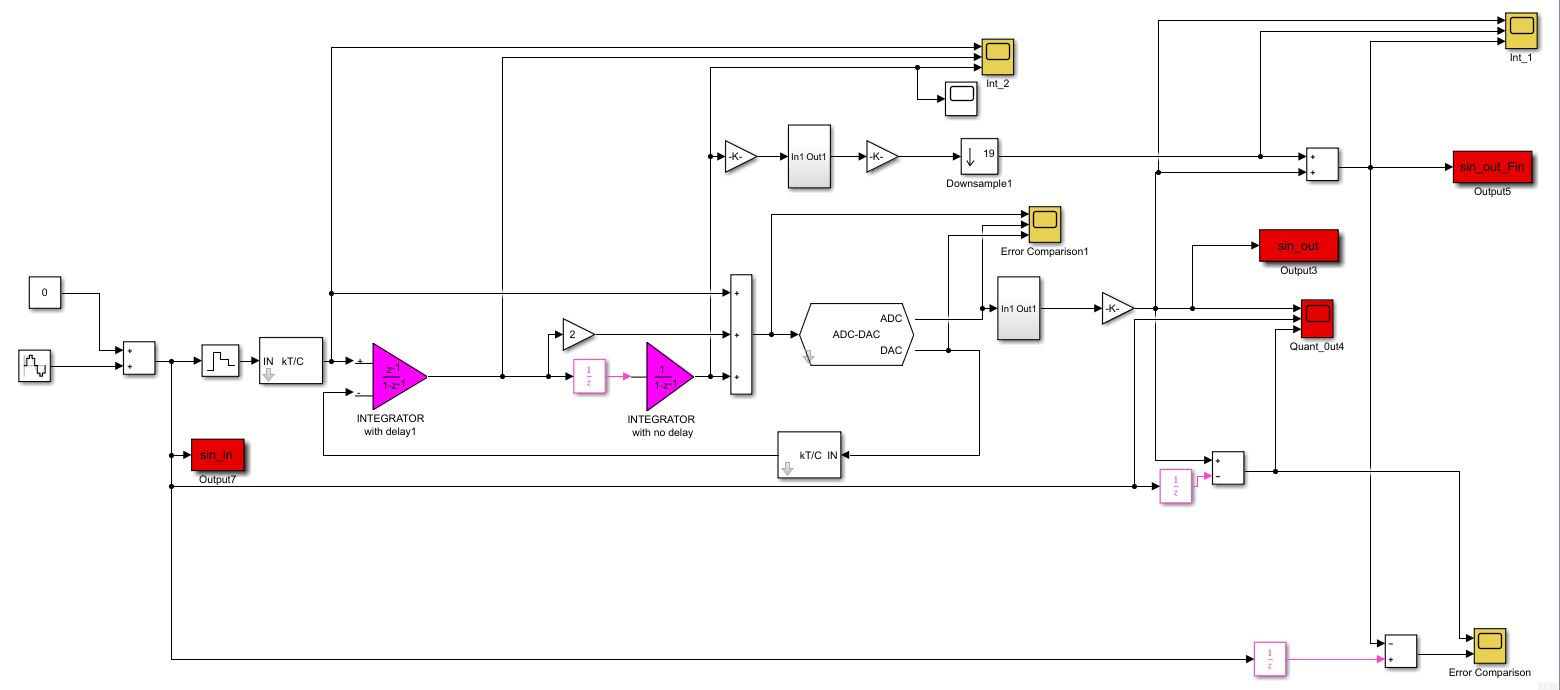
\includegraphics[width=\columnwidth]{Chap04/Figures/simulink_model_snapshot.jpg}
\caption{Simulink Model of Second Order Incremental Feed-forward Architecture of Sigma-Delta Modulator}
\label{SIM_ERISDM}
\end{figure}
Developed Simulink model architecture incorporates sample-and-hold, two delayed integrators, quantizer followed by decimation filter in the I{\textSigma}{\textDelta}M path, while residue signal digitization path comprised of gain block, residual quantizer and decimator as shown in the Fig. \ref{SIM_ERISDM}.
\section{Block Description:}
\subsection{Integrator Block:}
\begin{figure}[h]
\centering
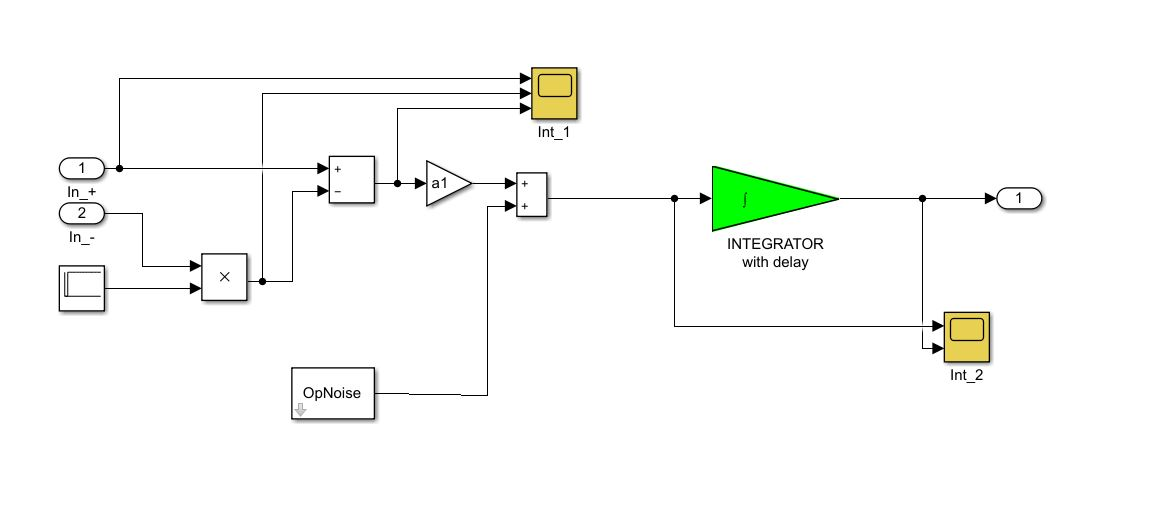
\includegraphics[width=\columnwidth]{Chap04/Figures/sim_first_integrator.JPG}
\caption{Simulink Model of the Integrators employed in the I{\textSigma}{\textDelta}M architecture}
\label{SIM_INT1}
\end{figure}
Integrator block has been built in order to incorporate the RESET feature to ensure the incremental function of the structure. Then a coefficient can be set with the solution of gain block. Along with this, different non-idealities of the Op-Amp needed to be consolidated, e.g. op-amp noise is included by using a block `OpNoise' while the MATLAB functions are written to encompass other non-idealities like slew rate, loop gain and Gain-Bandwidth Product inside the `INTEGRATOR with delay' block. The simulink model of the integrator is shown in the Fig. \ref{SIM_INT1}
For the ideal simulation, these parameters are set to, $Gain = 100\ dB$, $Slew\ Rate = 1\ V/ns$ and $GBW = 1\ GHz$ so the integrator reflects all the ideal characteristics.

\subsection{Quantizer:}
`ADC-DAC' block from the SDtoolbox library allows to specify the number of comparators, mismatch parameter along with total capacitance to be used in the quantizer e.g. for 2 bit quantizer i.e. 4 level quantizer, the required comparators are 3, while that for 3 level quantizer are 2 and so on.

\subsection{Decimation Filter:}
\begin{figure}[h]
\centering
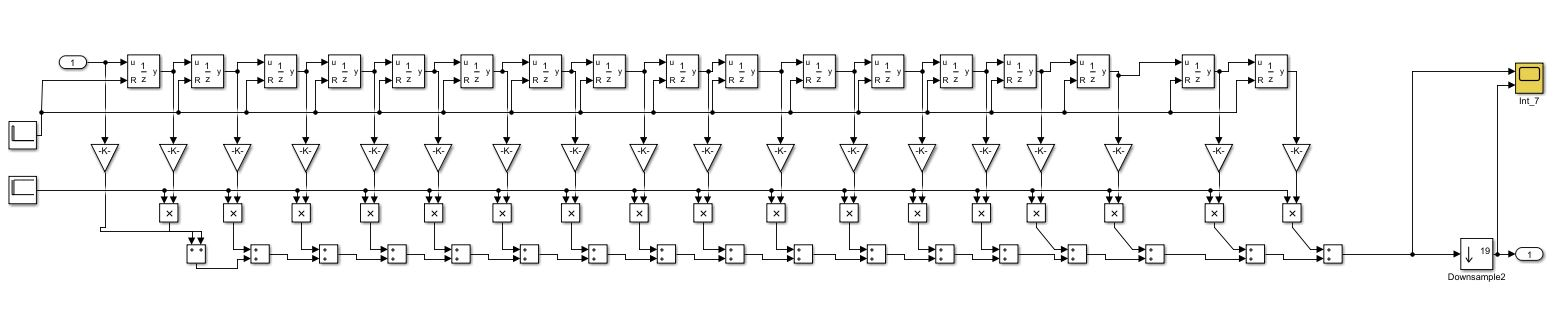
\includegraphics[width=\columnwidth]{Chap04/Figures/dec_filt.JPG}
\caption{Simulink Model of the Decimation Filter}
\label{SIM_DECFILT}
\end{figure}
Decimation filter block is the combination of the Finite Impulse Response (FIR) filter with decimator block. The FIR filter transfer function can be expressed as,
\begin{equation}
    H(Z) = a_0 + a_1Z^{-1} + a_2Z^{-2} + ...... + a_{M-1}Z^{\left(M-1\right)}
\end{equation}
which is implemented with $M$ number of gain blocks, $\left(M-1\right)$ number of delay elements and $\left(M-1\right)$ number of adders as shown in Fig.\ref{SIM_DECFILT}, where M is the over sampling ratio. The decimator block followed by FIR filter, samples the output of the filter after every M number of clock cycles.

\section{Analysis of Op-Amp Requirements}
 %%%%%%%%%%%%%%%%%%%%%%%%%%%%%%%%%%%%%%%%%%%%%%%%%%%%%%%%%%%%%%%%%%%%%%%%%%%%%%%%%%%%%%%%
Different combinations of resolution in IADC with a given value of $M$ and ERADC can fulfill a specific ENOB requirement. However, the sensitivity of each combination to the op-amp non-idealities varies, while selection of the optimum solution is necessary for robust performance. Therefore, the analysis of the op-amp specifications plays a very important role in selecting the best combination. The effects of op-amp non-idealities, such as gain and gain-bandwidth product (GBW), are, therefore, determined for an extended-range IADC with the combinations of resolution in IADC and ERADC summarized in Tab.~\ref{PARAM}, using a Simulink model.

A complete model of the Incremental {\textSigma}{\textDelta} Modulator with extended counting (Extended Range Incremental {\textSigma}{\textDelta} Modulator) is developed in the simulink as shown in Fig. \ref{SIM_ERISDM}. All the parameters of the Op-Amps are set with intention to reflect the ideal characteristics of Op-Amp and simulations are carried out. Various permutations and combinations of the resolutions of the I{\textSigma}{\textDelta}M and Residual ADC can be verified for given clock frequency of 80 MHz, total conversion time of 25 clock cycles to attain the ideal overall performance in terms of ENOB of 12, 13 and 14 and the other parameters considered are given in the Tab.~\ref{PARAM}
However, the additional 12 dB margin of SNR or 2-bit of ENOB must be considered over the exact requirement of SNR or ENOB to accommodate parasitic effects and process corners degradation as a usual practice. 
% combining which to the required SNR makes it 86 dB. Therefore the model is structured in a fashion so that ideally it should exhibit overall SNR of 86 dB.


\begin{table}
\centering
\begin{tabular}{c|c|c|c|c|c|c|c|c|c}
\Xhline{4\arrayrulewidth}
\textbf{ENOB\textsubscript{TOT}} & \multicolumn{3}{c|}{\textbf{12}} & \multicolumn{3}{c|}{\textbf{13}} & \multicolumn{3}{c}{\textbf{14}} \\ \hline
\textbf{N\textsubscript{SD}} & 3 & 3 & 4 & 3 & 3 & 4 & 3 & 3 & 4 \\ \hline
\textbf{ENOB\textsubscript{INC}} & 12 & 9 & 10 & 13 & 9 & 10 & 14 & 9 & 10 \\ \hline
\textbf{N\textsubscript{RS}} & 0 & 3 & 2 & 0 & 4 & 3 & 0 & 5 & 4 \\ \hline
\textbf{M} & 45 & 18 & 18 & 64 & 18 & 18 & 90 & 18 & 18 \\ \Xhline{4\arrayrulewidth}
\end{tabular}
\caption{Parameters of the considered extended-range IADC}
\label{PARAM}
\end{table}

\subsection{Effect of Low-Frequency Gain}
The first parameter to be considered is the low-frequency gain of the op-amps used in the first and second integrator of the second-order IADC. The variation of the gain affects the integrator coefficient, as well as the location of the integrator pole. In a stand-alone IADC, the shift in the location of the pole has more significant effect than the modification of the integrator coefficient, since the integrator pole sets the zero of the IADC NTF. However, in an extended-range IADC also the variation of the integrator coefficient becomes important, since it affects the value of the residue and can cause a degradation of the overall performance after recombination. The integrator transfer function considering finite op-amp low-frequency gain is given by \cite{TCAS_MALCOVATI} 
\begin{equation}
    H(Z)=\frac{C_s}{C_f}\frac{Z^{-1}}{1-\alpha Z^{-1}}
\end{equation}
Parameter $\alpha$ is given by
\begin{equation}
    \alpha\approx\frac{A_0C_f}{A_0C_f+C_s}
\end{equation}
%%%%%%%%%%%%%%%%%%%%%%%%%%%%%%%%%%%%%%%%%%%%%%%%%%%%%%%%%%%%%%%%%%%%%%%%%%%%%%%%%%%%%
%    NEW EQUATION
%%%%%%%%%%%%%%%%%%%%%%%%%%%%%%%%%%%%%%%%%%%%%%%%%%%%%%%%%%%%%%%%%%%%%%%%%%%%%%%%%%%%
and integrator coefficient $a$ is given by
\begin{equation}
\begin{split}
    a &= \frac{A_0}{1+A_0\beta}\\
      &= \frac{A_0}{1+A_0\left(\frac{C_f}{C_s}\right)}\\
      &= \frac{1}{\left(\frac{1}{A_0}\right)+\left(\frac{C_f}{C_s}\right)}
    \label{INTEG_COEFF}
\end{split}
\end{equation}
%%%%%%%%%%%%%%%%%%%%%%%%%%%%%%%%%%%%%%%%%%%%%%%%%%%%%%%%%%%%%%%%%%%%%%%%%%%%%%%%%%%%
where $C_s$ is the sampling capacitance, $C_f$ is the feedback capacitance and $A_0$ is the op-amp low frequency gain.

%%%%%%%%%%%%%%%%%%%%%%%%%%%%%%%%%%%%%%%%%%%%%%%%%%%%%%%%%%%%%%%%%%%%%%%%%%%%%%%%%%%%%
%   NEW PARAGRAPH
%%%%%%%%%%%%%%%%%%%%%%%%%%%%%%%%%%%%%%%%%%%%%%%%%%%%%%%%%%%%%%%%%%%%%%%%%%%%%%%%%%%%%
From Eq. \ref{INTEG_COEFF}, it is clear that, for ideal op-amp with infinite gain ($A_0=\infty$), the integrator coefficient is simply a ratio of $C_s$ and $C_f$. However, finite low-frequency gain modifies the coefficient degrading the output signal. Therefore in case of second order IADC, the residue, when passed through and processed by series of two integrators, gets corrupted. Nevertheless, since the point at which the residue is injected, is actually a point of injection of the quantization error, the change in the residue value would get high-pass filtered as quantization noise, the corrupted value should be in certain limit though. Extended-range IADC, however, rely on the accuracy of the residue signal, as it is the input to the second stage ADC. If the estimate of residue itself turns out to be inappropriate, it's digital equivalent will also get inaccurate degrading the overall response significantly. This implies that the variation of integrator coefficient has significant effect in extended-range IADC than in standalone IADC.

In the case of feed-forward architecture of IADC, the output of the second integrator represents the residue $e[M]$ which can be expressed as,

\begin{equation}\label{RESIDUE_IDEAL}
    e[M]_{ideal} = a_1a_2\sum_{j=1}^{M}\sum_{k=1}^{j-1}u-a_1a_2V_{ref}\sum_{j=1}^{M}\sum_{k=1}^{j-1} v[k-1]
\end{equation}
 
 However, because of the finite gain of the op-amp, the equation changes to,
 \begin{equation*}
     \begin{split}
         e[M] = a_1a_2\sum_{j=1}^{M}\sum_{k=1}^{j-1}\alpha^{k-1}u-a_1a_2V_{ref}\sum_{j=1}^{M}\sum_{k=1}^{j-1} \alpha^{k-1}v[k-1]
     \end{split}
 \end{equation*}
 
  \begin{equation}\label{Vout_erisdm}
\begin{split}
     e[M]&=a_1a_2\left[\frac{\alpha^M-\alpha M+M-1}{\left(\alpha-1\right)^2}\right]u\\
         &-a_1a_2V_{ref}\left[\alpha^{M-2}v[M-2]+2\alpha^{M-3}v[M-2]+...+(M-2)\alpha v[1]+(M-1)v[0]\right]
\end{split}
\end{equation}

 
 \begin{align*}
     e[M]=First\ Term - Second\ Term
 \end{align*}
 
  
 \begin{align*}
     First\ Term = a_1a_2\left[\frac{\alpha^M-\alpha M+M-1}{\left(\alpha-1\right)^2}\right]u
 \end{align*}
 
 
 \begin{align*}
      \lim_{\alpha\to1} (First\ Term) =\lim_{\alpha\to1}a_1a_2\left[\frac{\alpha^M-\alpha M+M-1}{\left(\alpha-1\right)^2}\right]u
 \end{align*}
 
 After application of L-Hospital's Rule Two times,
 
 \begin{align*}
      \lim_{\alpha\to1} (First\ Term) =\lim_{\alpha\to1}a_1a_2\left[\frac{M(M-1)}{2}\alpha^{\left( M-2\right)}\right]u
 \end{align*}

 \begin{align*}
     First\ term\ error =\left.First\ Term\right|_{\alpha=1}-\left.First\ Term\right|_{\alpha}
 \end{align*}
 
 \begin{align*}
     First\ term\ error = a_1a_2\left[\frac{M(M-1)}{2}\right]u-a_1a_2\left[\frac{M(M-1)}{2}\alpha^{\left( M-2\right)}\right]u
 \end{align*}
 
 \begin{align*}
     First\ term\ error =a_1a_2\frac{M(M-1)}{2}\left[1-\alpha^{\left( M-2\right)}\right]u
 \end{align*}
 
  \begin{align} \label{FTE1}
     First\ term\ error \approx a_1a_2\frac{M^2}{2}\left[1-\alpha^{\left( M-2\right)}\right]u
 \end{align}
 
 Eq. \ref{FTE1} represents the approximate error on the input signal part of the residue, due to finite low-frequency gain.
  
 \begin{align*}
     Second\ term=a_1a_2V_{ref}&\left[\alpha^{M-2}v[M-2]+2\alpha^{M-3}v[M-2]+...\right.\\
                 &\left.+(M-2)\alpha v[1]+(M-1)v[0]\right]
 \end{align*}
 
   
 \begin{align*}
     Second\ term\ error =\left.Second\ Term\right|_{\alpha=1}-\left.Second\ Term\right|_{\alpha}
 \end{align*}
 
%  \begin{align*}
%      Second\ term\ error &=a_1a_2V_{ref}\left[v[M-2]+2v[M-2]+...+(M-2) v[1]+(M-1)v[0]\right]\\
%      &-a_1a_2V_{ref}\left[\alpha^{M-2}v[M-2]+2\alpha^{M-3}v[M-2]+...+(M-2)\alpha v[1]+(M-1)v[0]\right]
%  \end{align*}
 
 \begin{align*}
     Second\ term\ error=a_1a_2V_{ref}&\left[(1-\alpha^{M-2})v[M-2]+2(1-\alpha^{M-3})v[M-2]+...\right.\\
                                      &\left.+(M-2)(1-\alpha) v[1]\right]
 \end{align*}
 
 \begin{align*}
     Second\ term\ error= a_1a_2V_{ref}\sum_{j=1}^{M}\sum_{k=1}^{j-1} \left(1-\alpha^{k-1}\right)v[k-1]
 \end{align*}
 
  
 \begin{equation}
     \begin{split}
         Error_{e[M]}&\approx a_1a_2\frac{M^2}{2}\left[1-\alpha^{\left( M-2\right)}\right]u\\&-a_1a_2V_{ref}\sum_{j=1}^{M}\sum_{k=1}^{j-1} \left(1-\alpha^{k-1}\right)v[k-1]
     \end{split}
 \end{equation}
 
 Here, the error introduced due to the Low-frequency gain of the op-amp varies sample-to-sample. However, a moderate assumption and/or approximation can be made to make the calculation simple that the residue is corrupted by $[1-\alpha^{(\frac{M-2}{2})}]$ instead, then above equation can be modified as,
 
  \begin{equation}
     \begin{split}
         Error_{e[M]}\approx a_1a_2\frac{M^2}{2}\left[1-\alpha^{\left( \frac{M}{2}-1\right)}\right]u-a_1a_2V_{ref}\left[1-\alpha^{\left( \frac{M}{2}-1\right)}\right]\sum_{j=1}^{M}\sum_{k=1}^{j-1} v[k-1]
     \end{split}
 \end{equation}
 
   \begin{equation}
     \begin{split}
         Error_{e[M]}\approx \left[1-\alpha^{\left( \frac{M}{2}-1\right)}\right]\left[a_1a_2\frac{M^2}{2}u-a_1a_2V_{ref}\sum_{j=1}^{M}\sum_{k=1}^{j-1} v[k-1]\right]
     \end{split}
 \end{equation}
 
 Now the second term is actually a residue (eq.(\ref{RESIDUE_IDEAL})) whose peak value is nothing but the step-size of the IADC. Then it can be expressed as,
 
 \begin{align*}
    e[M]_{ideal}=\left[a_1a_2\frac{M^2}{2}u-a_1a_2V_{ref}\sum_{j=1}^{M}\sum_{k=1}^{j-1} v[k-1]\right]=\frac{2}{M(M-1)}\frac{V_{ref}}{\left(2^{N_{SD}}-1\right)}
\end{align*}


\begin{align}
    Error_{e[M]}\approx\frac{2}{M(M-1)}\frac{V_{ref}}{\left(2^{N_{SD}}-1\right)}\left[1-\alpha^{\left( \frac{M}{2}-1\right)}\right]
\end{align}

This is the peak value of the error on the residue which adds power to the quantization noise and in turn reduces the SNR value. Assuming the distribution of this error uniform, the rms value can be given as,

\begin{align}
    Error_{e[M]_{rms}}\approx\frac{1}{\sqrt{3}}\frac{2}{M(M-1)}\frac{V_{ref}}{\left(2^{N_{SD}}-1\right)}\left[1-\alpha^{\left( \frac{M}{2}-1\right)}\right]
\end{align}

Where, $\alpha = \left(1-\frac{1}{A_0}\right)$,

\begin{align}\label{ERROR_RMS}
    Error_{e[M]_{rms}}\approx\frac{1}{\sqrt{3}}\frac{2}{M(M-1)}\frac{V_{ref}}{\left(2^{N_{SD}}-1\right)}\left[1-\left(1-\frac{1}{A_0}\right)^{\left( \frac{M}{2}-1\right)}\right]
\end{align}

Then, the Signal-to-noise Ratio accounting for this error can be given as,

\begin{equation}\label{SNR}
    SNR = \frac{V_{sig_{rms}}^{2}}{Q_{eradc_{rms}}^2+Error_{e[M]_{rms}}^2}
\end{equation}

where $Q_{rms}$ is the RMS value of the quantization error of the overall architecture and $V_{sigrms}$ is the rms value of the input signal. Ideally, the error on the residue $Error_{e[M]}$ should be zero, and in practice, it should very small compared to the overall quantization noise (i.e. $Q_{eradc}$) of the Extended-Range architecture, i.e.


 \begin{align} \label{COMP_ERR}
     Error_{e[M]_{rms}}\ll Q_{eradc_{rms}}
 \end{align}
 
where, $Q_{eradc_{rms}}$ is given by,

 \begin{align}\label{QN_ERADC}
     Q_{eradc_{rms}}=\frac{1}{2\sqrt{3}}\frac{2}{M(M-1)}\frac{V_{ref}}{\left(2^{N_{SD}}-1\right)\left(2^{N_{RS}}-1\right)}
 \end{align}


\begin{figure}
    \centering
    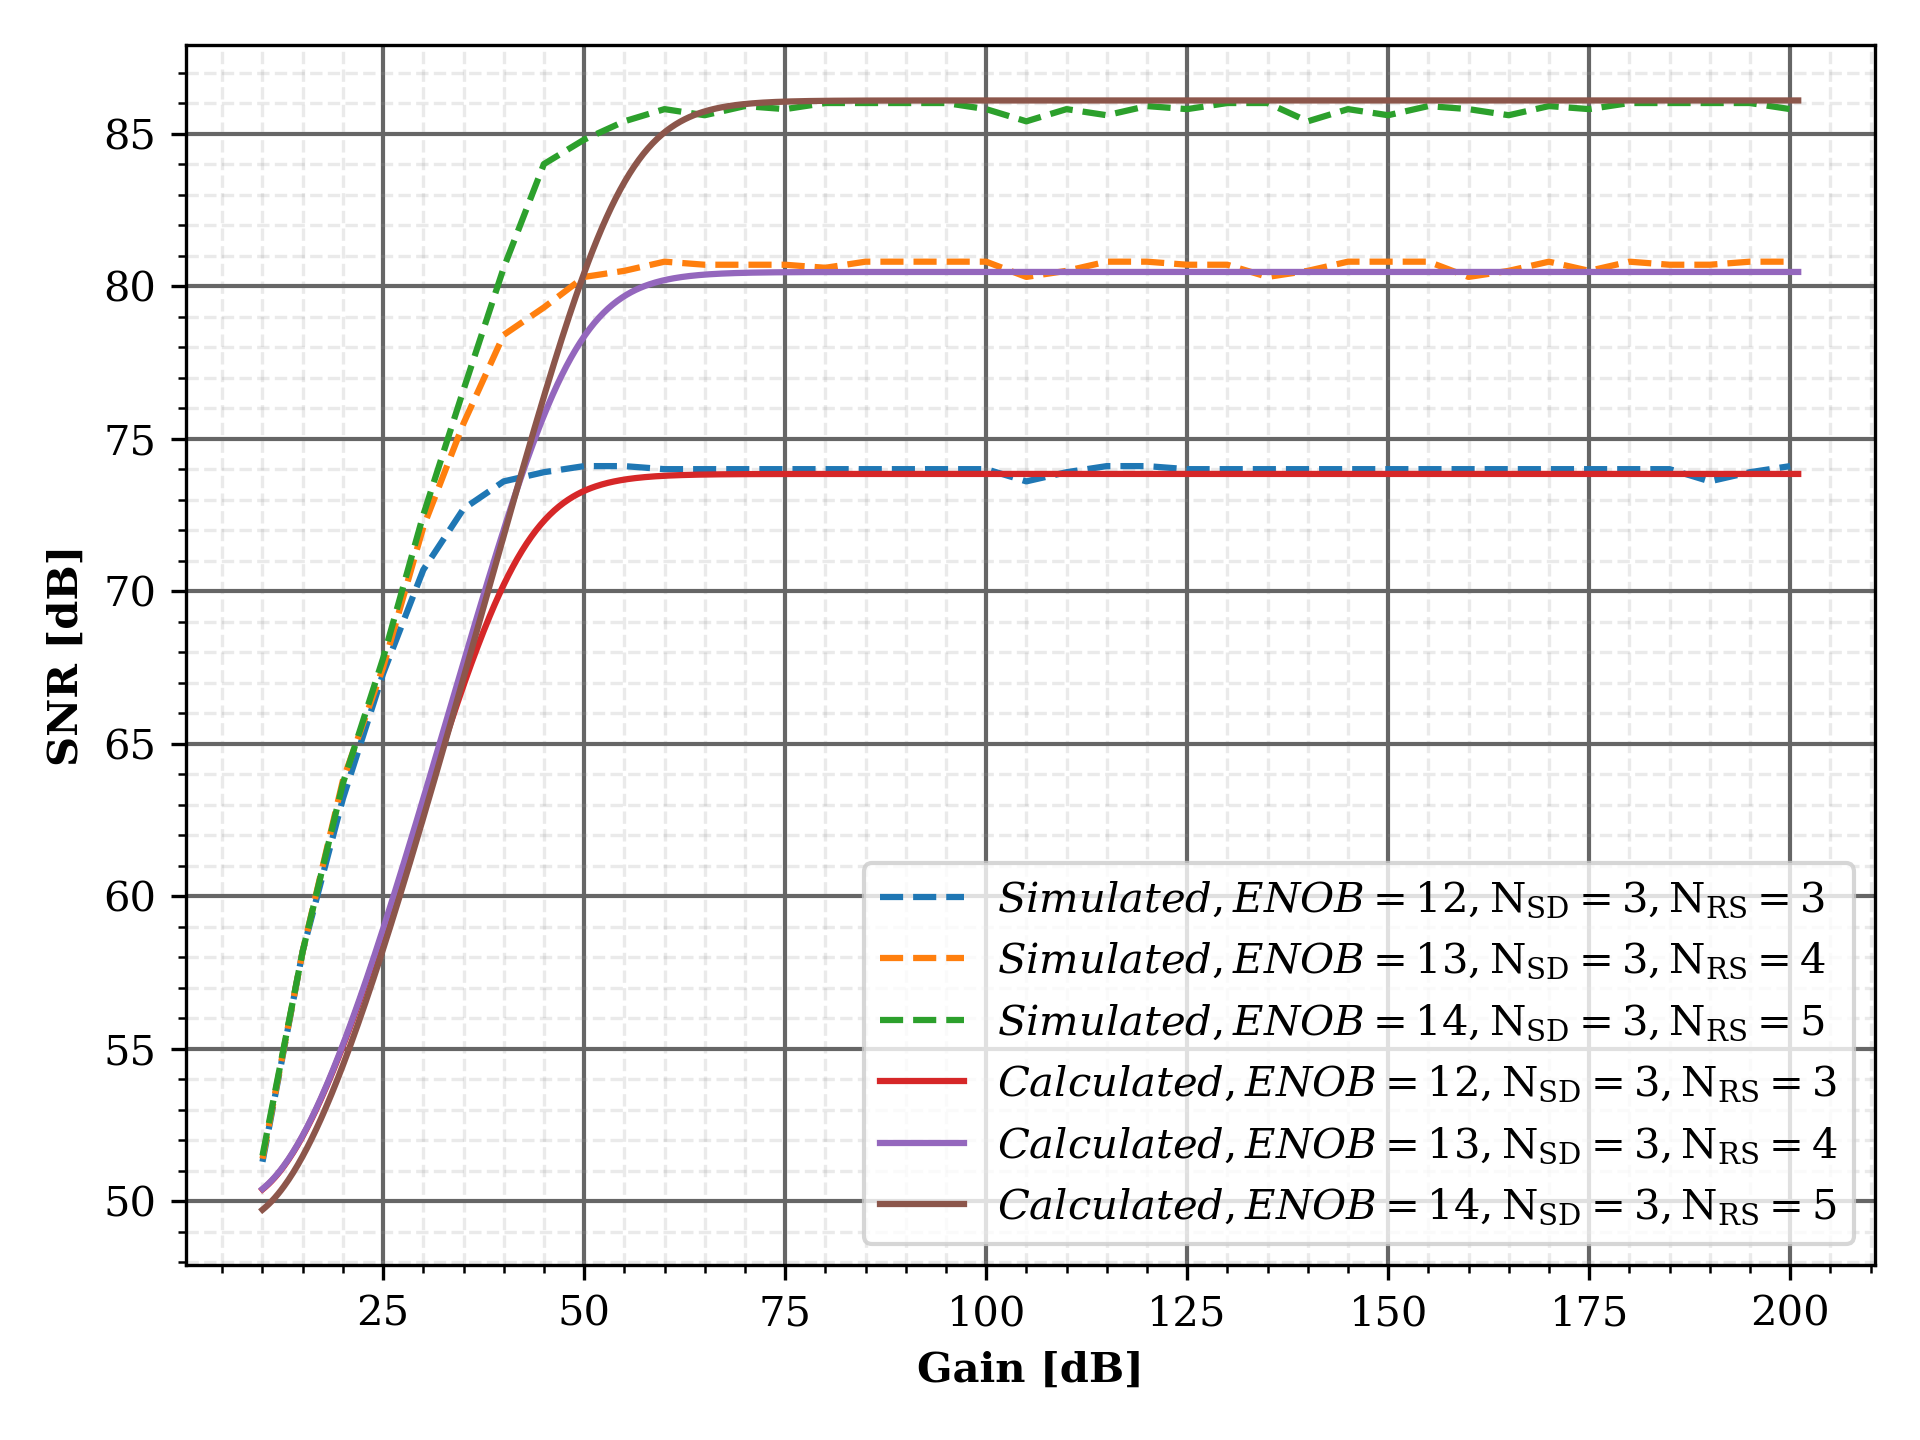
\includegraphics[scale=.7]{Chap04/Figures/snr_vs_gain_sim_calc}
    \caption{Simulated and Calculated SNR as a function of Low-frequency gain}
    \label{fig:SNR_G_calc}
\end{figure}

In order to validate the expression derived for $Error_{e[M]}$, a fair approach would be to plot the SNR as a function of $A_0$ using the equations (\ref{ERROR_RMS}), (\ref{SNR}) and (\ref{QN_ERADC}) and see how closely, the expression represents the actual simulated SNR. Fig. \ref{fig:SNR_G_calc} sows the comparison. Various resolutions in the residual ADC ($N_{RS}$) are considered while keeping the resolution of the quantizer in IADC $N_{SD} = 3$, oversampling ratio $M = 18$, keeping other non-idealities to reflect the ideal behavior and varying the gain from 10~dB to 200~dB. The dotted characteristic represents simulated cases while the solid ones are plotted with the expression derived. It is clear from the plot that both the graphs are close enough within the range of nearly 1~dB at a point when simulated one just reaches it's maximum value. For example, consider a case with SNR of 86~dB or ENOB of 14. When the simulated (dotted-green) characteristic attains it's maximum value of 86~dB at a gain of 60~dB, the calculated value (solid-brown characteristic) of SNR is 85~dB. Furthermore, the value of gain at which even the expression causes SNR to reach the maximum value is 65~dB, which is higher than the simulated one (60~dB).

A further step would be to derive the expression for the Low-frequency gain of the op-amp such that the eq.(\ref{COMP_ERR}) holds. Let's assume the factor $K$ such a that, 

 \begin{align} \label{COMP_ERR1}
     Error_{e[M]_{rms}} = \frac{Q_{eradc_{rms}}}{K}
 \end{align}

where factor $K$ is large enough so that eq.(\ref{COMP_ERR}) holds. Then, putting eq.(\ref{ERROR_RMS}) and eq.(\ref{QN_ERADC}) in eq.(\ref{COMP_ERR1}),

 \begin{align*}
    \frac{1}{\sqrt{3}}\frac{2}{M(M-1)}\frac{V_{ref}}{\left(2^{N_{SD}}-1\right)}\left[1-\alpha^{\left( \frac{M}{2}-1\right)}\right]=\frac{1}{2\sqrt{3}K}\frac{2}{M(M-1)}\frac{V_{ref}}{\left(2^{N_{SD}}-1\right)\left(2^{N_{RS}}-1\right)}
\end{align*}

\begin{align*}
    \left[1-\alpha^{\left( \frac{M}{2}-1\right)}\right]=\frac{1}{2K\left(2^{N_{RS}}-1\right)}
\end{align*}

\begin{align*}
    1-\frac{1}{2K\left(2^{N_{RS}}-1\right)}=\alpha^{\left( \frac{M}{2}-1\right)}
\end{align*}

\begin{align*}
    \alpha^{\left( \frac{M}{2}-1\right)}=1-\frac{1}{2K\left(2^{N_{RS}}-1\right)}
\end{align*}

\begin{align*}
    \alpha=\left[1-\frac{1}{2K\left(2^{N_{RS}}-1\right)}\right]^{\left(\frac{1}{\frac{M}{2}-1}\right)}
\end{align*}

\begin{align*}
    1-\frac{1}{A_0}=\left[1-\frac{1}{2K\left(2^{N_{RS}}-1\right)}\right]^{\left(\frac{2}{M-2}\right)}
\end{align*}


\begin{align*}
  1-\left[1-\frac{1}{2K\left(2^{N_{RS}}-1\right)}\right]^{\left(\frac{2}{M-2}\right)}=\frac{1}{A_0}
\end{align*}

\begin{align*}
    A_0=\frac{1}{1-\left[1-\frac{1}{2K\left(2^{N_{RS}}-1\right)}\right]^{\left(\frac{2}{M-2}\right)}}
\end{align*}

\begin{align}\label{A1}
    A_0(dB)= 20\log_{10}\left\{\frac{1}{1-\left[1-\frac{1}{2K\left(2^{N_{RS}}-1\right)}\right]^{\left(\frac{2}{M-2}\right)}}\right\}
\end{align}

% \begin{align}\label{A1}
%     A_0(dB)\approx 20\log_{10}\left[\frac{1}{1-\left(\frac{2^{N_{RS}+1}-3}{2^{N_{RS}+1}-2}\right)^{\left(\frac{2}{M}\right)}}\right]
% \end{align}

 \begin{figure}
    \centering
    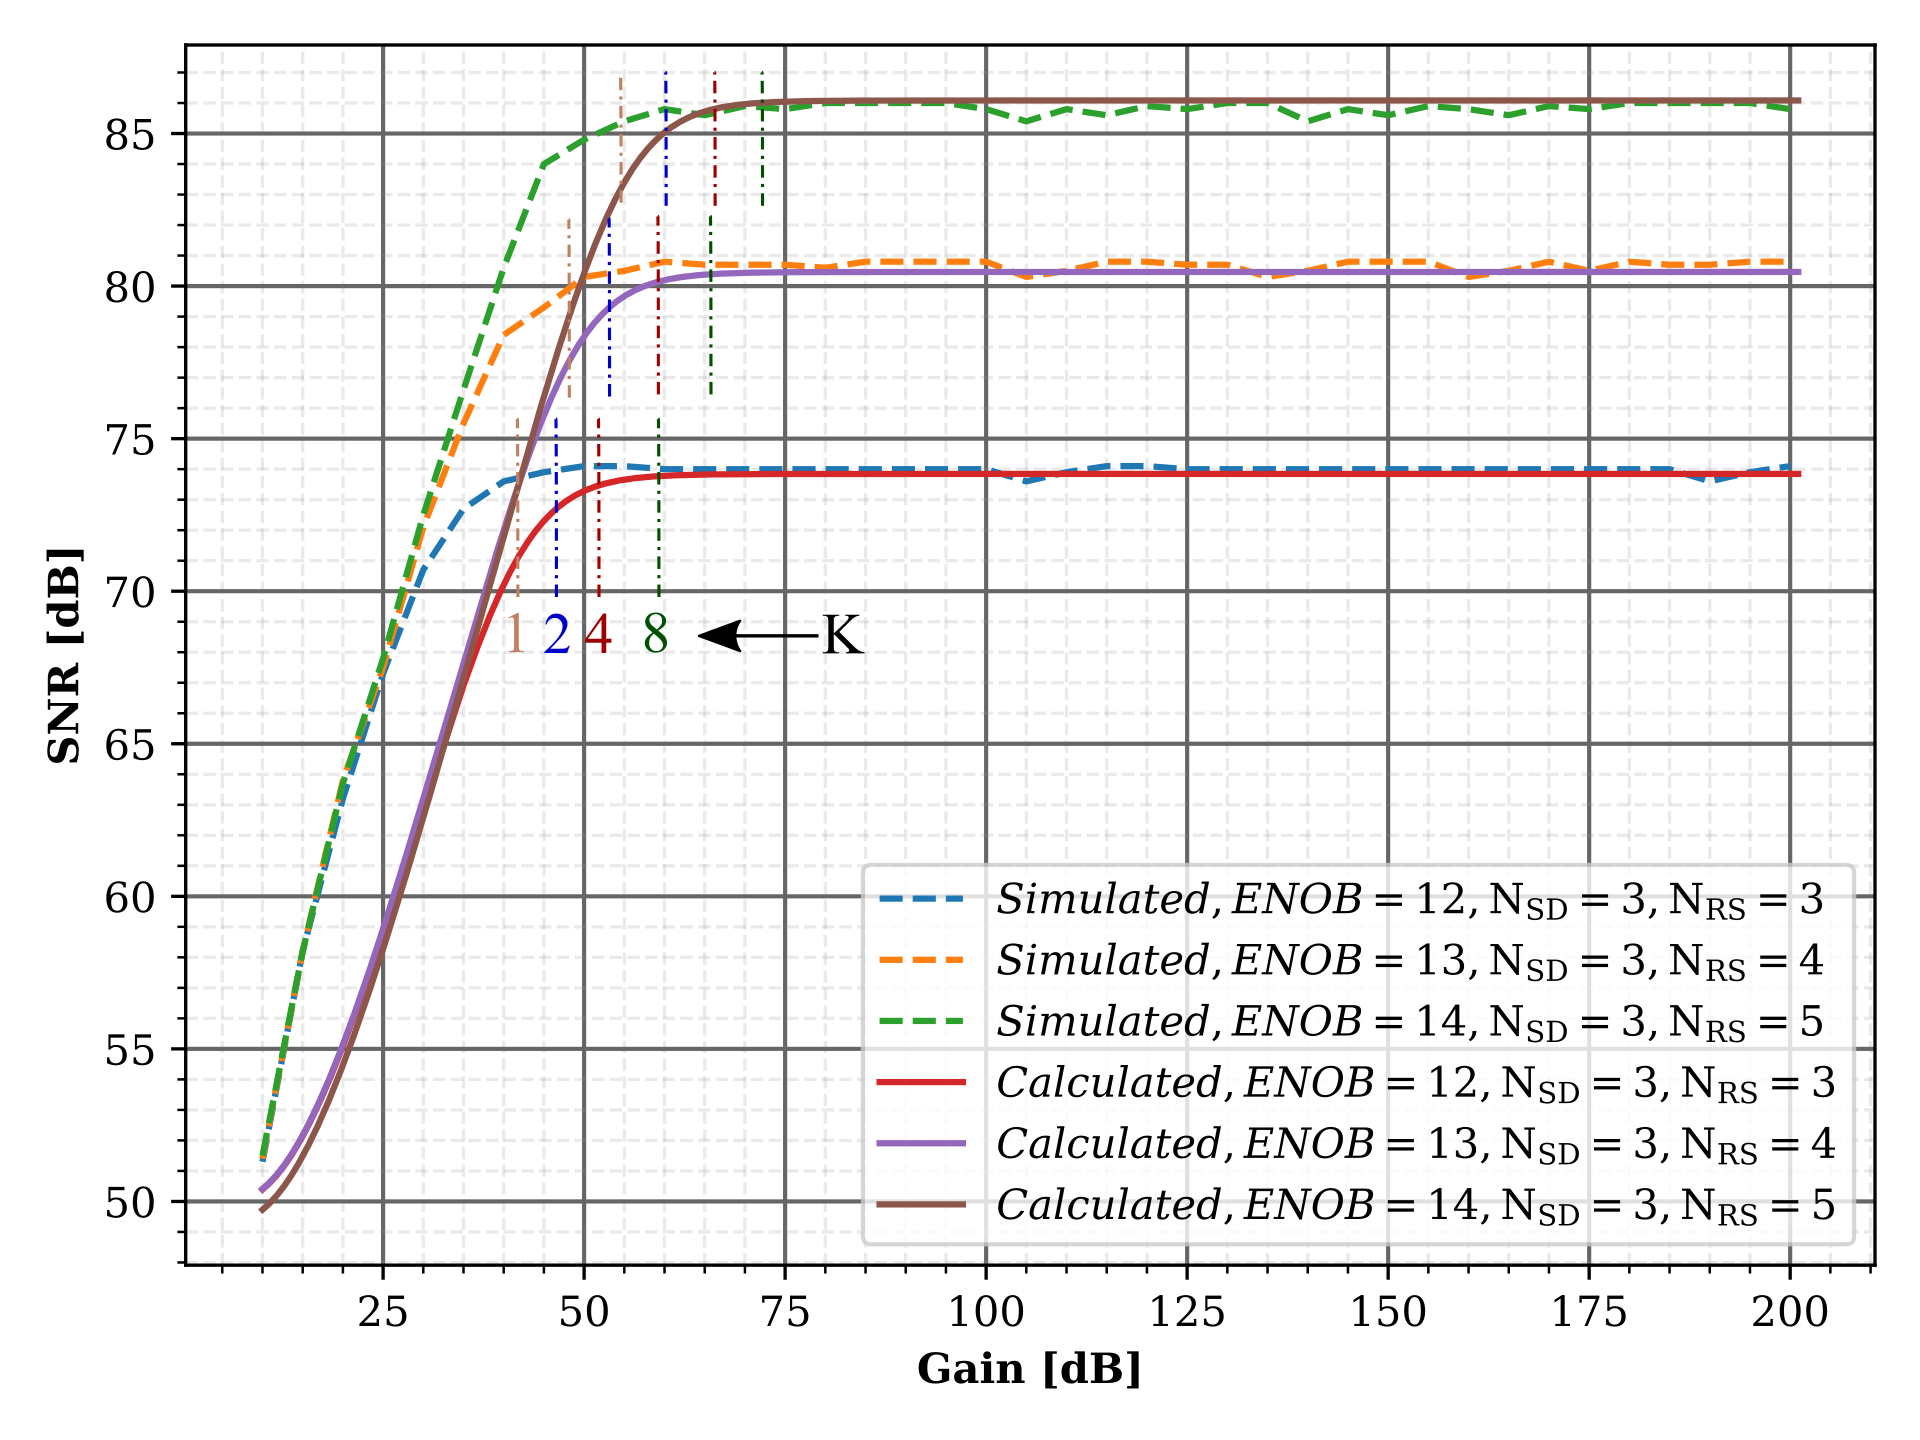
\includegraphics[scale=.7]{Chap04/Figures/snr_vs_gain_calc1}
    \caption{Simulated and Calculated SNR as a function of Low-frequency gain}
    \label{fig:SNR_G_calc1}
\end{figure}

Fig.\ref{fig:SNR_G_calc1} shows the SNR Vs low-frequency gain plot for various resolutions of the RADC for different values of $K$. When $K$ is 1, the error on the residue is actually half the overall quantization noise. Therefore, the Signal-to-noise ratio at that point will have a value less by $3~dB$ than it's maximum value (from eq(\ref{SNR})) on the calculated characteristic, however on the simulated one, it's right at the edge where it reaches it's maximum value. So, $A_{3dB_{calc}} = A_{max_{sim}}$. Nevertheless, a reasonable assumption of the factor $K$ would be 8 where both the curves attains the maximum SNR while leaving some margin on the gain for the process corners and mismatch variation.

% Please add the following required packages to your document preamble:
% \usepackage{multirow}
% Please add the following required packages to your document preamble:
% \usepackage{multirow}
\begin{table}[h]
\centering
\resizebox{\textwidth}{!}{
% Please add the following required packages to your document preamble:
% \usepackage{multirow}
\begin{tabular}{c|c|c|c|c|c|c|c|c|c|c|c|c}
\Xhline{5\arrayrulewidth}
\multirow{2}{*}{\textbf{N\textsubscript{RS}}} & \multicolumn{3}{c|}{\textbf{K=1}}       & \multicolumn{3}{c|}{\textbf{K=2}}       & \multicolumn{3}{c|}{\textbf{K=4}}       & \multicolumn{3}{c}{\textbf{K=8}}       \\ \cline{2-13} 
                     & \textbf{Gain}  & \textbf{SNR\textsubscript{sim}} & \textbf{SNR\textsubscript{calc}} & \textbf{Gain}  & \textbf{SNR\textsubscript{sim}} & \textbf{SNR\textsubscript{calc}} & \textbf{Gain}  & \textbf{SNR\textsubscript{sim}} & \textbf{SNR\textsubscript{calc}} & \textbf{Gain}  & \textbf{SNR\textsubscript{sim}} & \textbf{SNR\textsubscript{calc}} \\ \hline
3                    & 40.7  & 73.5      & 71.2       & 46.87 & 74        & 72.8       & 52.95 & 74        & 73.5       & 58.89 & 74        & 74         \\ \hline
4                    & 47.47 & 80        & 77.6       & 53.56 & 80.5      & 79.5       & 59.61 & 80.9      & 80.1       & 65.65 & 80.9      & 80.8       \\ \hline
5                    & 53.84 & 85.1      & 82.2       & 59.9  & 85.8      & 85         & 65.93 & 85.7      & 85.5       & 71.96 & 85.8      & 85.8       \\ \Xhline{5\arrayrulewidth}
\end{tabular}
}
\caption{Comparison between the Simulated and Calculated SNR (in dB) for different values of $K$ as a function of Low-frequency gain in (dB)}
\label{tab:SIM_CALC_COMP}
\end{table}

The comparison between the simulated SNR and the SNR on the modeled characteristic at a calculated gain using eq (\ref{A1}) has been shown in Tab. \ref{tab:SIM_CALC_COMP} for different values of $K$. For $K=1$ the SNR on the modeled characteristic at calculated gain from eq (\ref{A1}) have the values 3~dB down the maximum SNR. Increasing $K$ brings the calculated SNR values very close to the simulated ones while for $K=8$ both simulated and calculated SNR values are equal. Nevertheless considering $K=8$ for the gain calculation would be advantageous in order to account for even process variations and mismatch.

%%%%%%%%%%%%%%%%%%%%%%%%%%%%%%%%%%%%%%%%%%%%%%%%%%%%%%%%%%%%%%%%%%%%%%%%%%%%%%%%%%%%%
\subsubsection{Low-Frequency Gain of the First-Integrator Op-Amp}
The low-frequency gain of the first integrator op-amp in the IADC is varied from 0~dB to 100~dB considering the IADC standalone and extended-range architectures with the parameters shown in Table \ref{PARAM}. In Fig. \ref{SNR_G1}, the achieved SNR is plotted as a function of the op-amp gain for ENOB requirement of 12, 13 and 14 bit, respectively.

\begin{figure}[h]
\centering
\subfigure[]{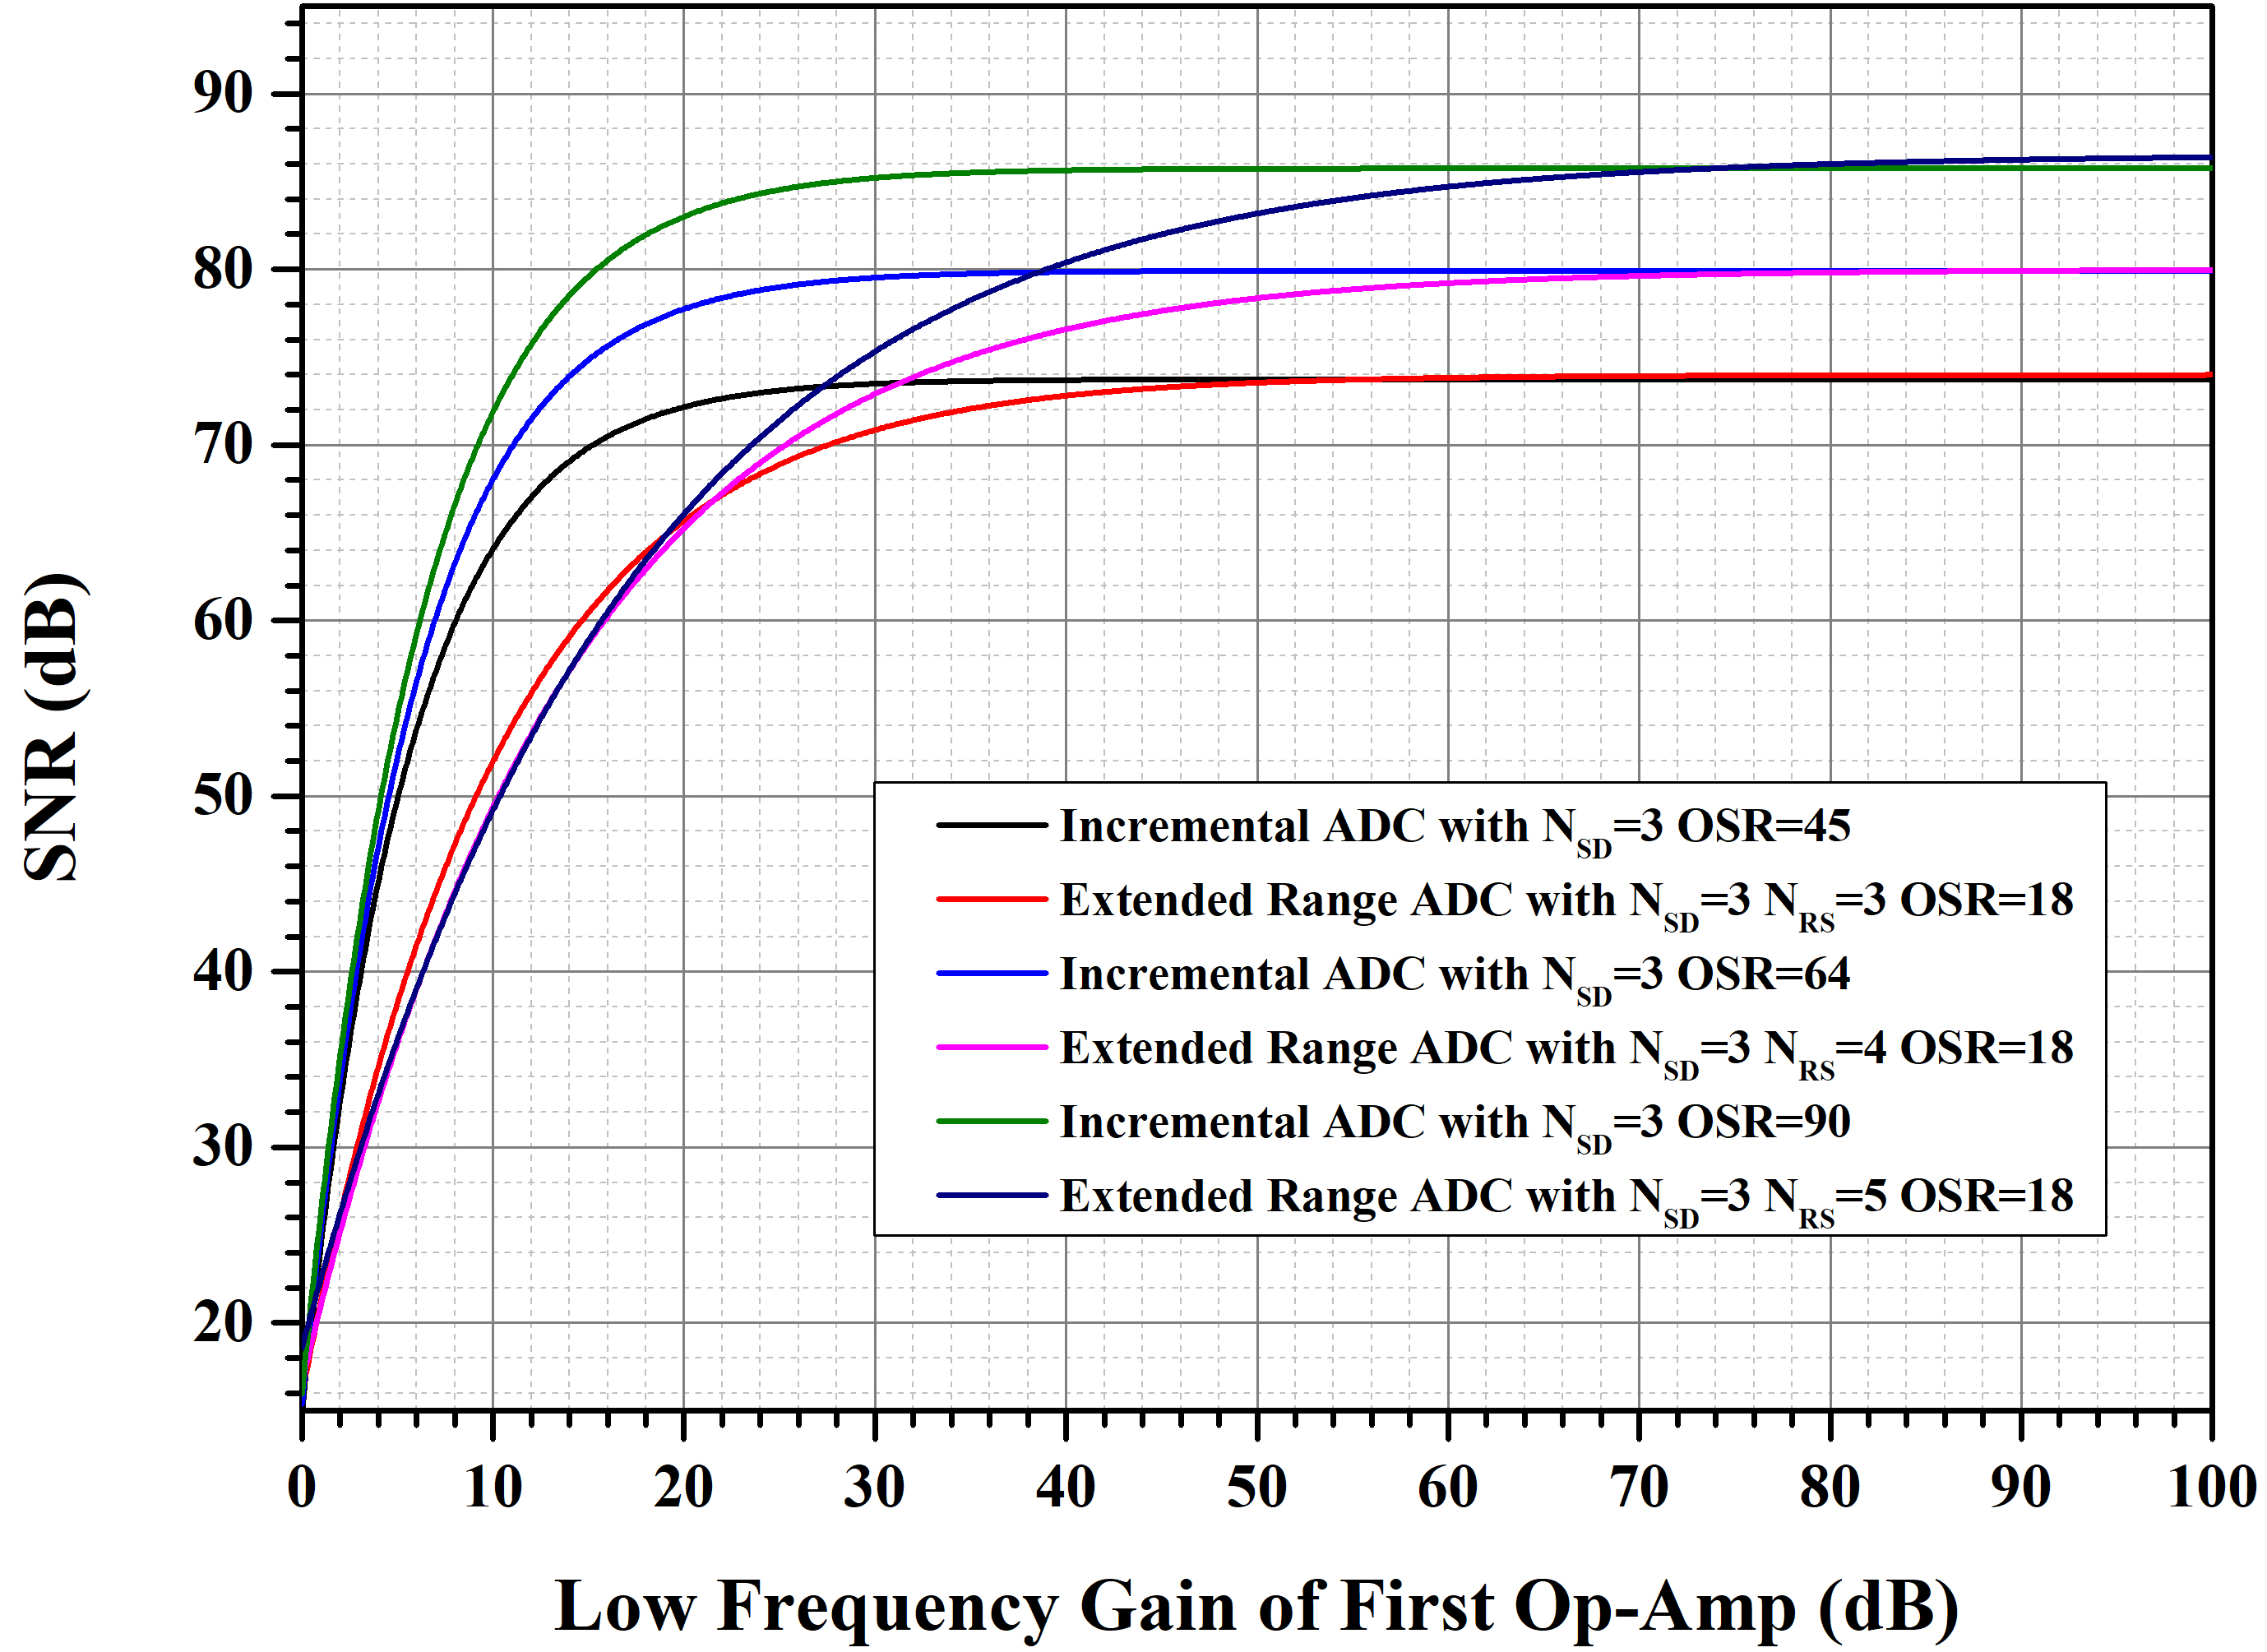
\includegraphics[scale=.28]{Chap04/Figures/SNR_G1_NSD3}}
\qquad
\subfigure[]{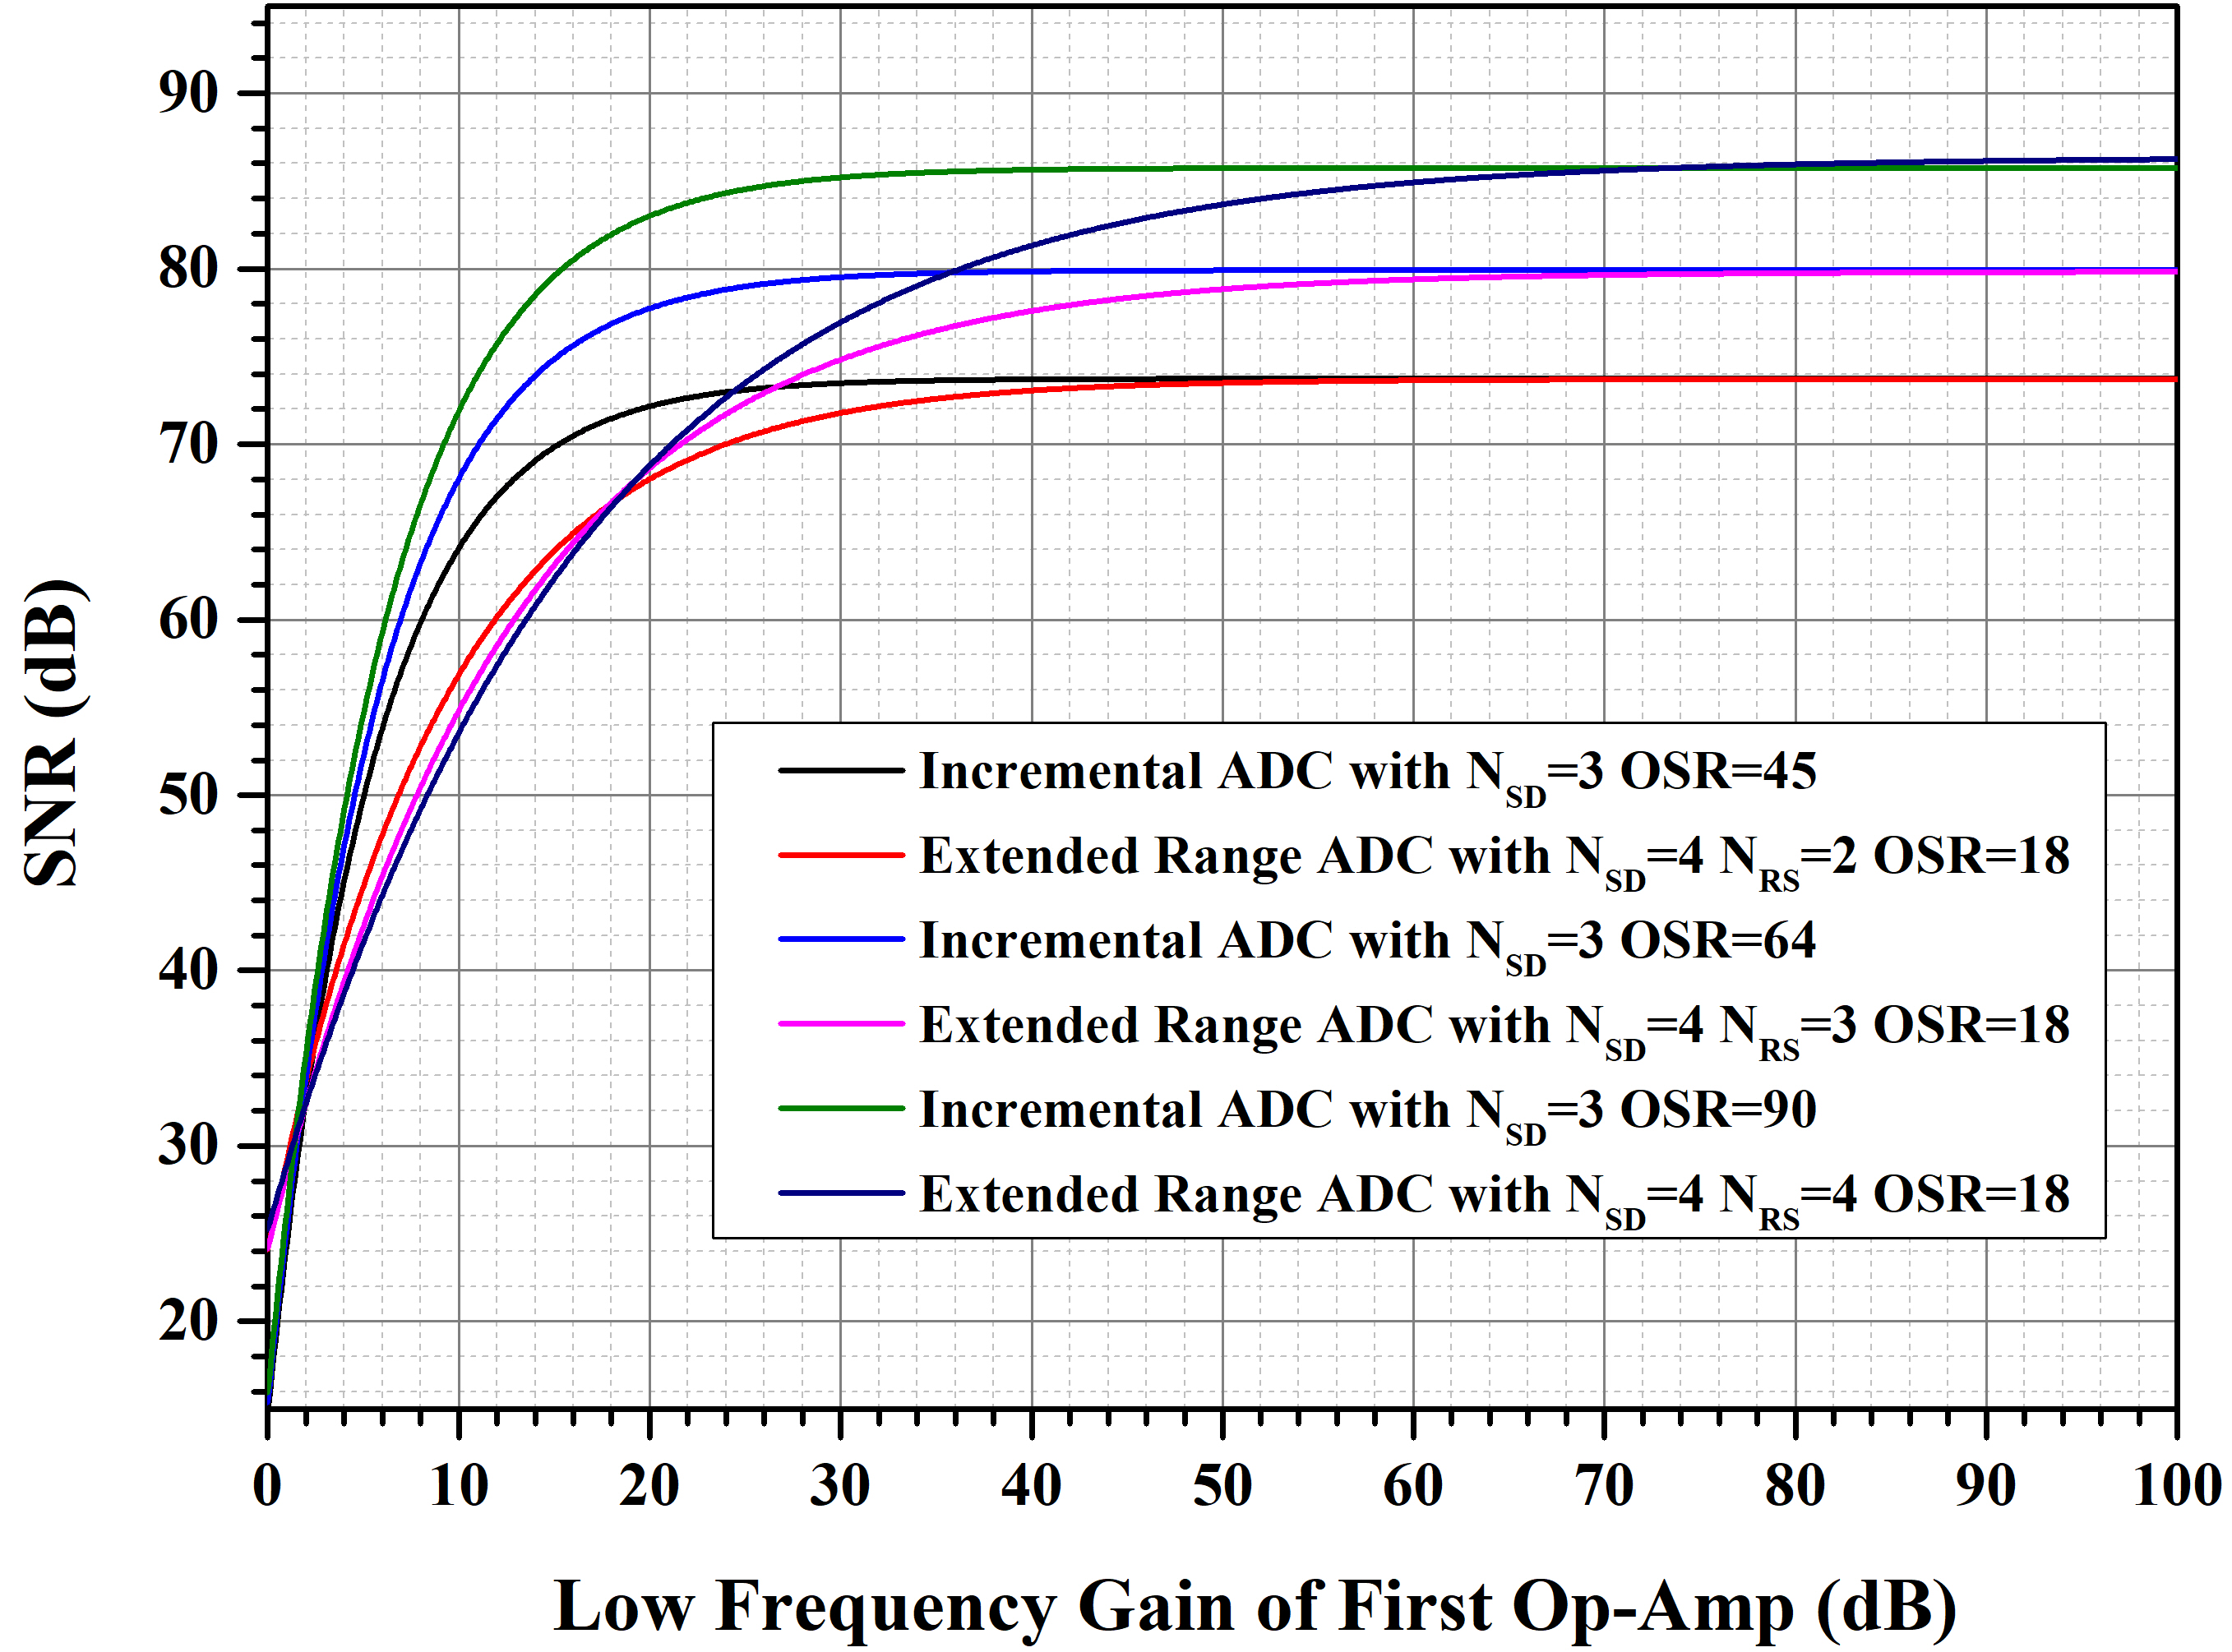
\includegraphics[scale=.28]{Chap04/Figures/SNR_G1_NSD4}}
\caption{Comparison of the IADC and extended-range IADC with different values of the first-integrator op-amp gain}
\label{SNR_G1}
\end{figure}


It can be observed that for the standalone IADC, the gain requirement is low and almost equal for all the three ENOB values, while in case of extended range IADC the gain requirement is considerably higher and increases as the ENOB requirement increases. The minimum gain needed for the IADC to achieve an SNR of 86~dB is around 40~dB, while that for the extended-range IADC it is around 70~dB. Obviously the conversion time for the extended-range IADC is much shorter than for the standalone IADC (less clock cycles are required).


\subsubsection{Low-Frequency Gain of the Second-Integrator Op-Amp}
The impact of the low-frequency gain of the second-integrator op-amp on the overall performance is negligible in standalone IADCs, but it turn out to be critical for extended-range IADCs, since it affects the integrator coefficient and, hence, the residue value. Fig. \ref{SNR_G2} shows this effect.
\begin{figure}[h]
\centering
\subfigure[]{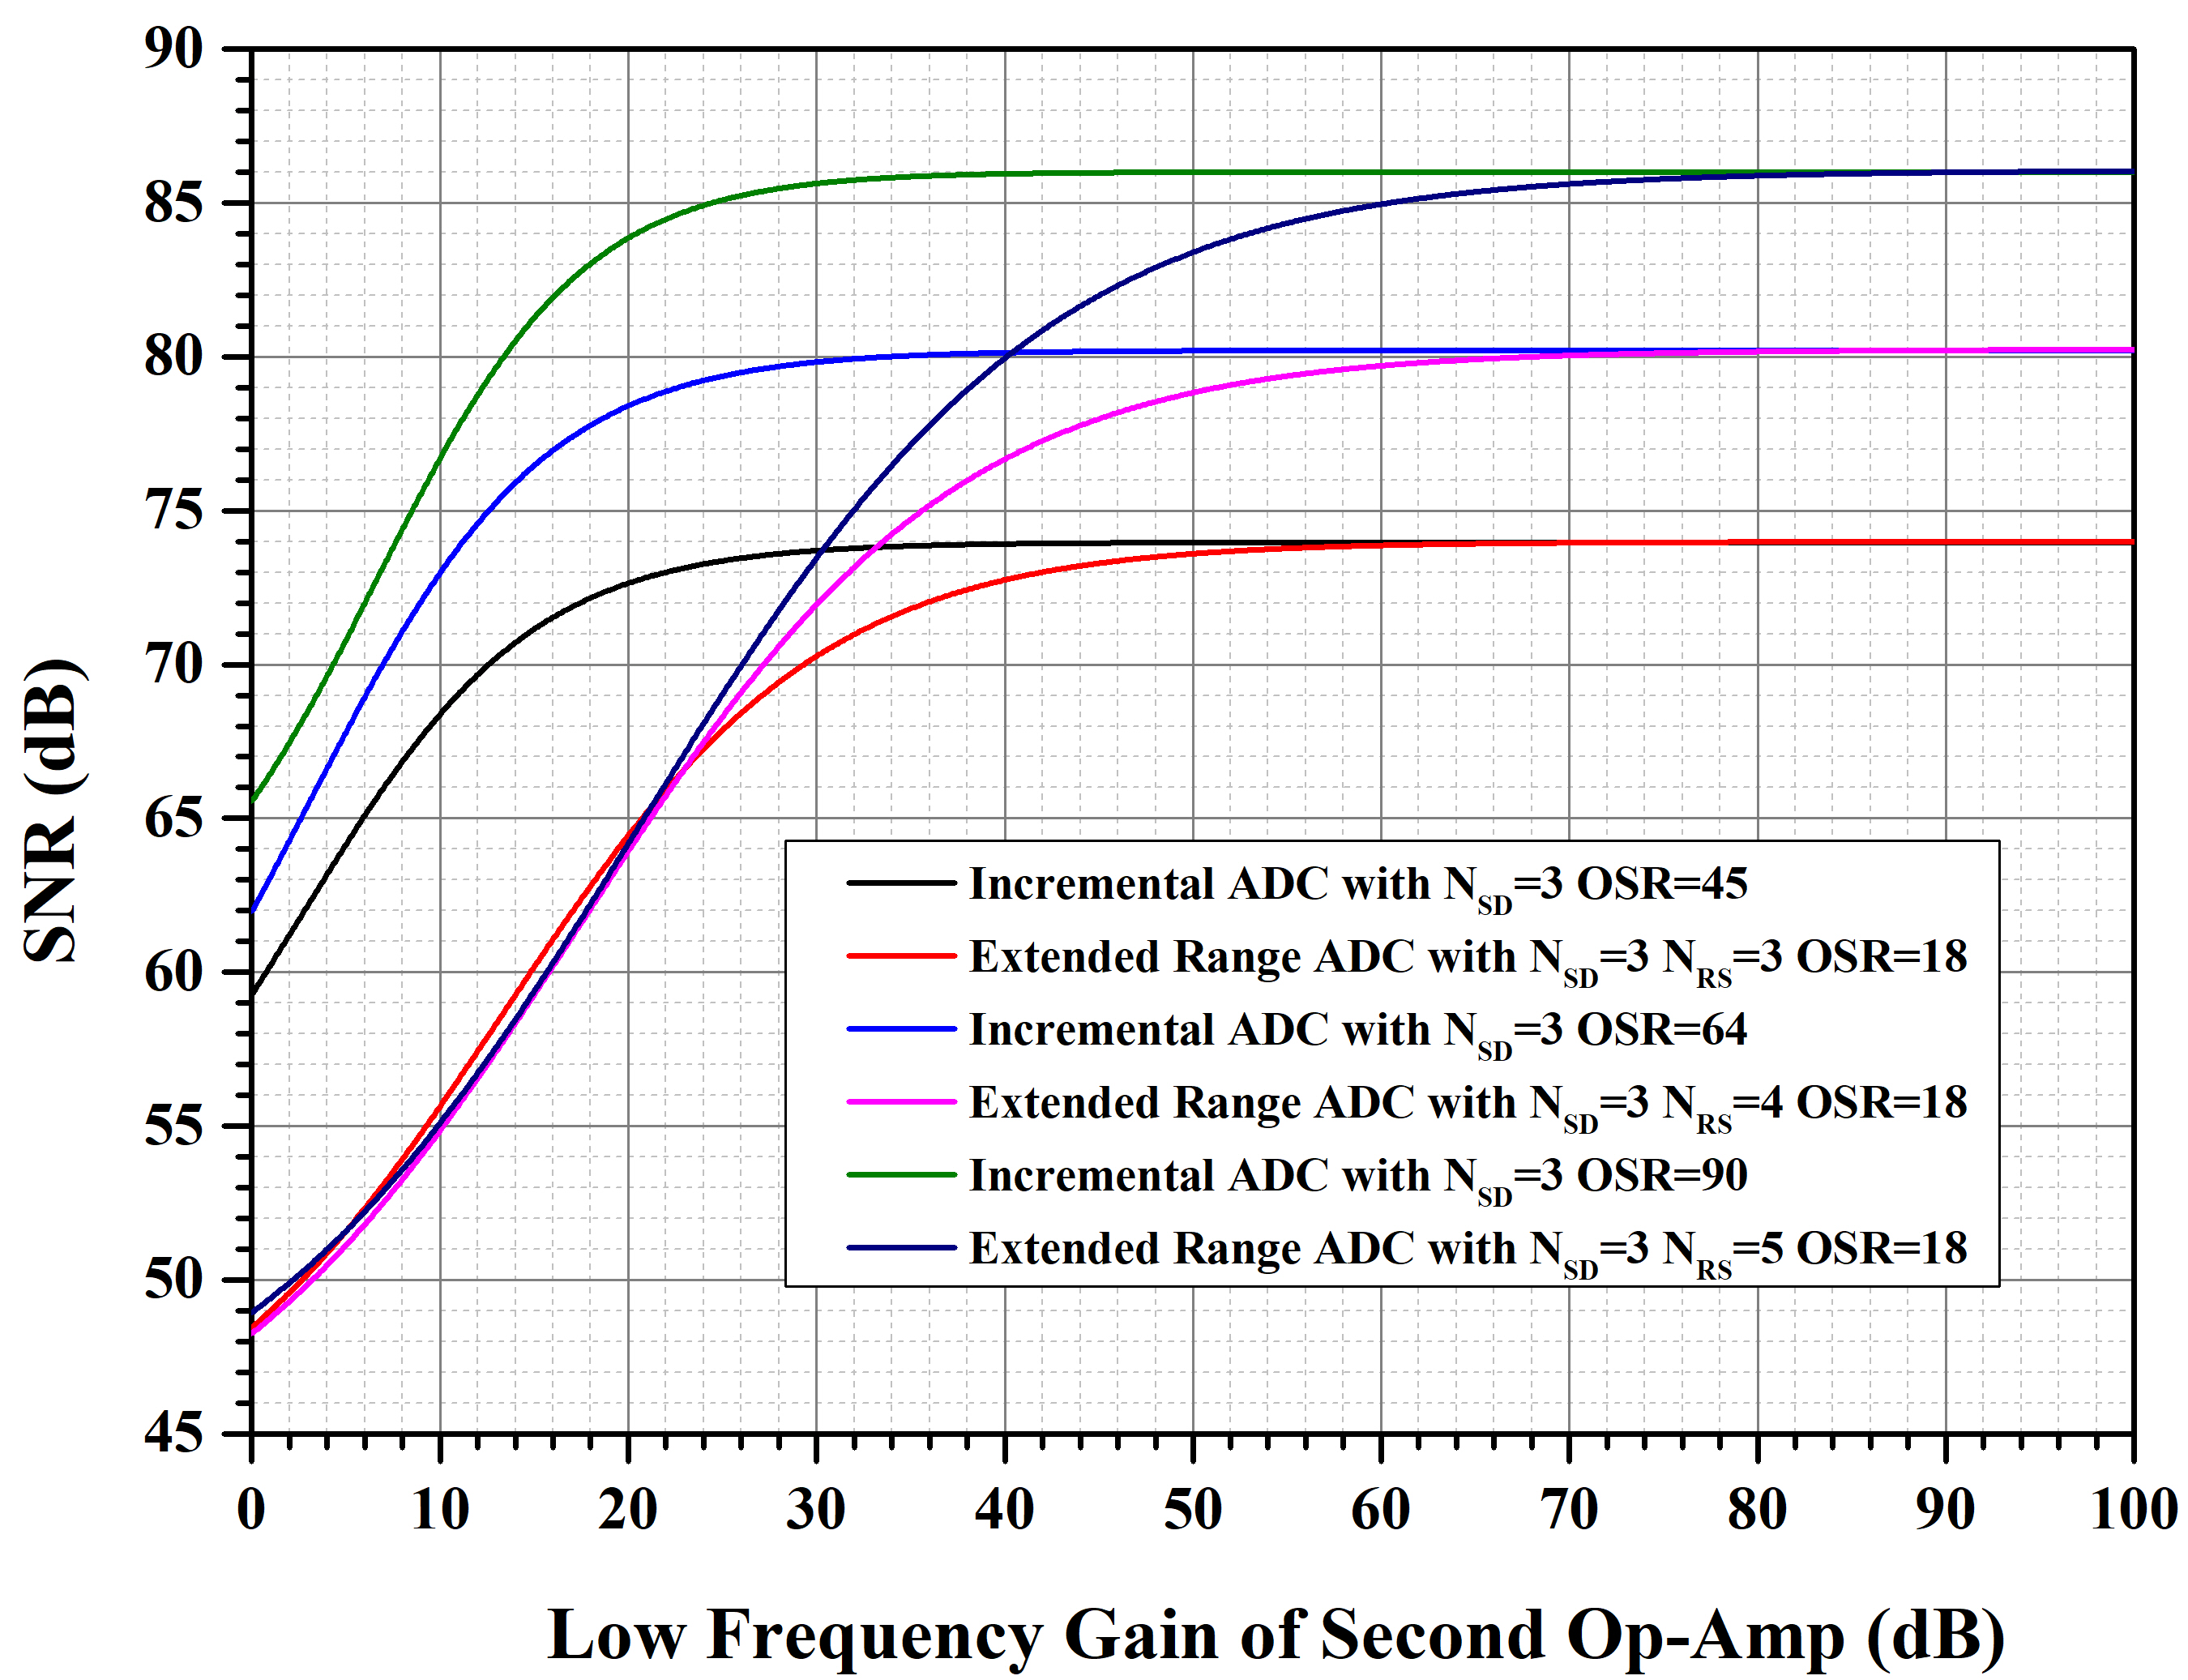
\includegraphics[scale=.28]{Chap04/Figures/SNR_G2_NSD3}}
\qquad
\subfigure[]{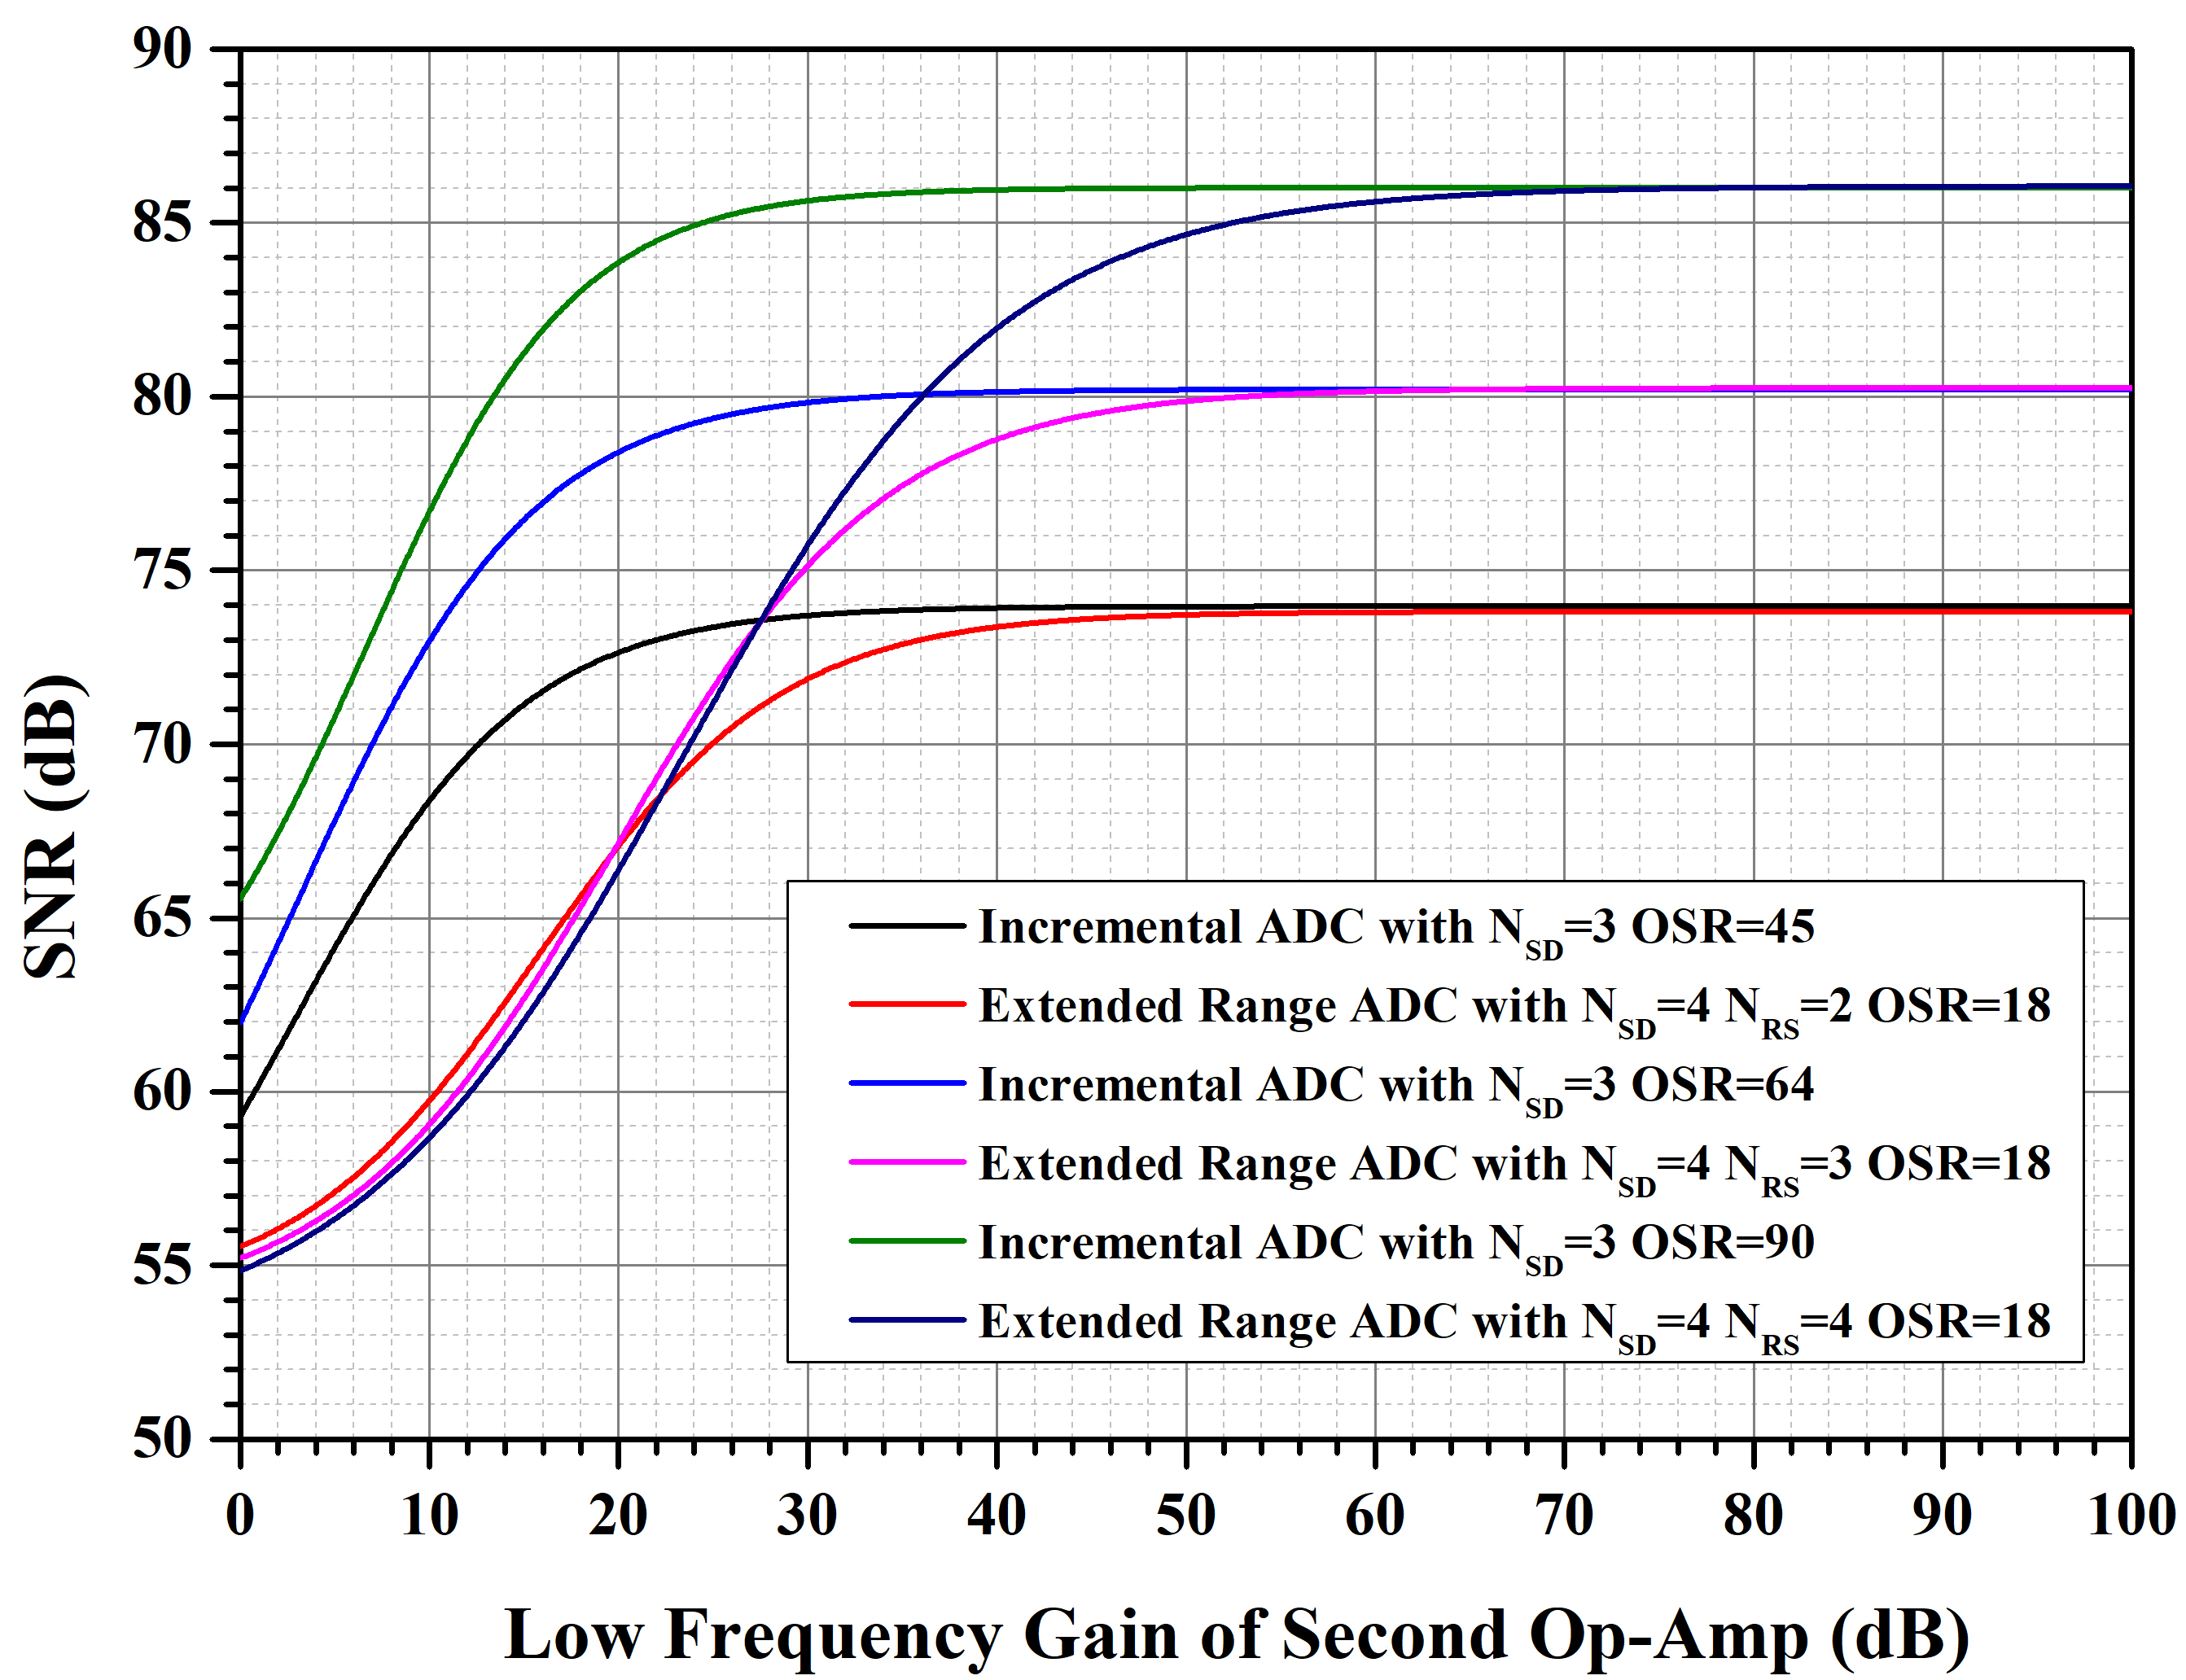
\includegraphics[scale=.28]{Chap04/Figures/SNR_G2_NSD4}}
\caption{Comparison of the IADC and extended-range IADC with different values of the second-integrator op-amp gain}
\label{SNR_G2}
\end{figure}


% %%%%%%%%%%%%%%%%%%%%%%%%%%%%%%%%%%%%%%%%%%%%%%%%%%%%%%%%%%%%%%%%%%%%%%%%%%%%%%%%%%%%%%%%%%%%%%%%%%%%%%%%%%%%%%%%%%%%
%  \begin{equation*}
%      \begin{split}
%          e[M]= a_1a_2\sum_{j=1}^{M}\alpha^j\sum_{k=1}^{j-1}u+a_1a_2V_{ref}\sum_{j=1}^{M}\alpha^j\sum_{k=1}^{j-1}v[k-1]
%      \end{split}
%  \end{equation*}
 
%  \begin{align*}
%      e[M] = First\ Term + Second\ Term
%  \end{align*}
%  %%%%%%%%%%%%%%%%%%%%%%%%%%%%%%%%%%%%%%%%%%%%%%%%%%%%%%%%%%%%%%%%%%%%%%%%%%%%%%%%%%%%%%%%%%%%%%

 
%  \begin{align*}
%      First\ Term = a_1a_2\sum_{j=1}^{M}\alpha^j\sum_{k=1}^{j-1}u
%  \end{align*}
 
%  \begin{align*}
%      First\ Term = a_1a_2u\sum_{j=1}^{M}\alpha^j\left(j-1\right)
%  \end{align*}
 
%  \begin{align*}
%      First\ Term = a_1a_2u\frac{(M-1)\alpha^{M+2}-M\alpha^{M+1}+\alpha^2}{(\alpha-1)^{2}}
%  \end{align*}
 
%  L-Hospital Rule two times as $\alpha \to 1$,
 
%  \begin{align*}
%      First\ Term = a_1a_2u\frac{(M-1)(M+1)(M+2)\alpha^{M}-M^2(M+1)\alpha^{M-1}+2}{2}
%  \end{align*}
 
% \textcolor{red}{$\alpha^{M}\approx\alpha^{M-1}$} Then,
 
%  \begin{align*}
%      First\ Term \approx a_1a_2u\frac{(M-1)(M+1)(M+2)\alpha^{M}-M^2(M+1)\alpha^{M}+2}{2}
%  \end{align*}
 
%  \begin{align*}
%      First\ Term \approx a_1a_2u\frac{(M+1)\alpha^{M}[(M+2)(M-1)-M^2]}{2}
%  \end{align*}
 
%  \begin{align*}
%      First\ Term \approx a_1a_2u\frac{(M+1)(M-2)\alpha^{M}}{2}
%  \end{align*}
 
%  \begin{align*}
%      First\ Term \approx a_1a_2\frac{M^2}{2}\alpha^{M}u
%  \end{align*}
 
%  \begin{align*}
%      First\ term\ error \approx a_1a_2\frac{M^2}{2}\left[1-\alpha^{M}\right]u
%  \end{align*}
 
 
%  %%%%%%%%%%%%%%%%%%%%%%%%%%%%%%%%%%%%%%%%%%%%%%%%%%%%%%%%%%%%%%%%%%%%%%%%%%%%%%%%%%%%%%%%%%%%%%%%%%%%%%%%%%%%%%%%%%%%%%%%%%%%%%%%%%%%%%%%%%%%%
 


% \begin{align*}
%     Second\ Term = a_1a_2V_{ref}\sum_{j=1}^{M}\alpha^j\sum_{k=1}^{j-1}v[k-1]
% \end{align*}
 
 
%  \begin{equation*}
%  \begin{split}
%      Second\ Term= a_1a_2V_{ref}\left[&\alpha^Mv[M-2] \right. \\
%                                       +&(\alpha^M+\alpha^{M-1})v[M-3]\\
%                                       +&(\alpha^M+\alpha^{M-1}+\alpha^{M-2})v[M-4]\\
%                                       +&...............................................\\
%                                       +&\left.(\alpha^M+\alpha^{M-1}+\alpha^{M-2}+....+\alpha^2)v[0]\right]
%  \end{split}
%  \end{equation*}
 
%  \begin{equation*}
%  \begin{split}
%      Second\ Term\ error = a_1a_2V_{ref}\left[&(1-\alpha^M)v[M-2] \right. \\
%                                       +&(2-(\alpha^M+\alpha^{M-1}))v[M-3]\\
%                                       +&(3-(\alpha^M+\alpha^{M-1}+\alpha^{M-2}))v[M-4]\\
%                                       +&...............................................\\
%                                       +&\left.((M-2)-(\alpha^M+\alpha^{M-1}+\alpha^{M-2}+....+\alpha^2))v[0]\right]
%  \end{split}
%  \end{equation*}
 
%   \begin{equation*}
%  \begin{split}
%      Second\ Term\ error = a_1a_2V_{ref}\left[&(1-\alpha^M)v[M-2] \right. \\
%                                       +&2\left(1-\frac{\alpha^M+\alpha^{M-1}}{2}\right)v[M-3]\\
%                                       +&3\left(1-\frac{\alpha^M+\alpha^{M-1}+\alpha^{M-2}}{3}\right)v[M-4]\\
%                                       +&...............................................\\
%                                       +&\left.(M-2)\left(1-\frac{\alpha^M+\alpha^{M-1}+\alpha^{M-2}+....+\alpha^2}{(M-2)}\right)v[0]\right]
%  \end{split}
%  \end{equation*}
     
% The most dominant term in the error is $(1-\alpha^M)$. So, assuming worst case that, all the samples are affected equally with $(1-\alpha^M)$. Then,

% \begin{align*}
%     Second\ Term\ error \approx a_1a_2V_{ref}\left(1-\alpha^M\right)\sum_{j=1}^{M}\sum_{k=1}^{j-1}v[k-1]
% \end{align*}

% %%%%%%%%%%%%%%%%%%%%%%%%%%%%%%%%%%%%%%%%%%%%%%%%%%%%%%%%%%%%%%%%%%%%%%%%%%%%%%%%%%%%%%%%%%%%%%%%%%%%%%%%%%%%%%%%%%%%%%%%%%%%%%%%%%%%%%%%%%%%%%%%%%%%%%



% If we consider the assumptions made above, then the error in the residue can be expressed as in the following equation and then it's just a matter of replacing $\alpha^{M-2} \to \alpha^M$ in Eq.(\ref{A1}) and Eq.(\ref{GBW1}). 

% \begin{align*}
%      Error_{e[M]} \approx a_1a_2\frac{M^2}{2}\left[1-\alpha^{}\right]u-a_1a_2V_{ref}\left(1-\alpha^M\right)\sum_{j=1}^{M}\sum_{k=1}^{j-1}v[k-1]
%  \end{align*}
 
% \begin{align*}
%     Error_{e[M]}\approx\frac{2}{M(M-1)}\frac{V_{ref}}{\left(2^{N_{SD}}-1\right)}\left[1-\alpha^{M}\right]
% \end{align*}

% \begin{align*}
%     A_0(dB)\geq 20\log_{10}\left[\frac{1}{1-\left(\frac{2^{N_{RS}+1}-3}{2^{N_{RS}+1}-2}\right)^{\frac{1}{M}}}\right]
% \end{align*}


\subsection{Effect of Finite GBW of the Op-Amps}
Another major parameter which influences the ADC performance is the op-amp finite GBW. Finite GBW causes an incomplete charge transfer in the integrator at the end of each clock phase, leading to an error. A stand-alone IADC, is pretty robust against incomplete settling in the integrators. However, since the extended-range IADC performance relies on the accuracy of the residue value, which is obtained at the second integrator output, incomplete settling becomes quite detrimental for the overall ADC performance and, therefore, the op-amp GBW requirement becomes much more stringent. 

In order to study the dependence of the overall Gain-Bandwidth Product (GBW) of the first Op-Amp over the SNR, all the other parameters, including the Gain, are brought back to the ideal values and GBW of the first Op-Amp is varied from 30 MHz to 300 MHz as shown in Fig. \ref{GBW_Vs_SNR_NSD2}(a). To achieve the maximal stable SNR, the promising value of the GBW of the first op-amp could be 250 MHz. Similar procedure is followed to observe the effect of GBW of second op-amp on the comprehensive SNR and the response is plotted as shown in the Fig.\ref{GBW_Vs_SNR_NSD2}(b).

In case of error due to GBW, it is equivalent of change in the integrator coefficient $a$ by $\alpha a$, then, the output of the second integrator can be given as,

 
 \begin{equation*}
     \begin{split}
         e[M] = \alpha a_1a_2\sum_{j=1}^{M}\sum_{k=1}^{j-1}u-\alpha a_1a_2V_{ref}\sum_{j=1}^{M}\sum_{k=1}^{j-1}v[k-1]
     \end{split}
 \end{equation*}
 
The error on the residue due to finite GBW can be given as, 

\begin{equation*}
    Error_{e[M]} = \left.e[M]\right|_{\alpha=1} - \left.e[M]\right|_{\alpha}
\end{equation*}

 
 \begin{equation*}
     \begin{split}
         Error_{e[M]} = \left(1-\alpha\right) a_1a_2\sum_{j=1}^{M}\sum_{k=1}^{j-1}u-\left(1-\alpha\right) a_1a_2V_{ref}\sum_{j=1}^{M}\sum_{k=1}^{j-1}v[k-1]
     \end{split}
 \end{equation*}

\begin{figure}[ht]
    \centering
    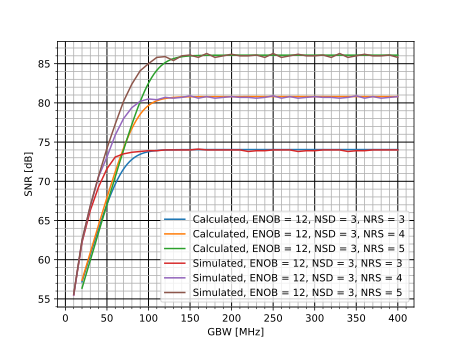
\includegraphics[scale=.7]{Chap04/Figures/snr_vs_gbw_sim_calc}
    \caption{Comparison between the simulated and modeled SNR equation w.r.t. GBW}
    \label{fig:SNR_GBW_calc}
\end{figure}

  
 \begin{equation*}
     \begin{split}
         Error_{e[M]} = \left(1-\alpha\right) \left[a_1a_2\sum_{j=1}^{M}\sum_{k=1}^{j-1}u- a_1a_2V_{ref}\sum_{j=1}^{M}\sum_{k=1}^{j-1}v[k-1]\right]
     \end{split}
 \end{equation*}
 
  \begin{align*}
    e[M]_{ideal}=\left[a_1a_2\sum_{j=1}^{M}\sum_{k=1}^{j-1}u-a_1a_2V_{ref}\sum_{j=1}^{M}\sum_{k=1}^{j-1} v[k-1]\right]=\frac{2}{M(M-1)}\frac{V_{ref}}{\left(2^{N_{SD}}-1\right)}
\end{align*}

\begin{equation*}
    Error_{e[M]}=\left(1-\alpha\right) \frac{2}{M(M-1)}\frac{V_{ref}}{\left(2^{N_{SD}}-1\right)}
\end{equation*}


This is the peak value of the error on the residue due to finite GBW. Assuming the uniform probability distribution function for the error, it's rms value can then be given as,

\begin{equation}
    Error_{e[M]_{rms}}=\frac{1}{\sqrt{3}}\frac{2}{M(M-1)}\frac{V_{ref}}{\left(2^{N_{SD}}-1\right)}\left(1-\alpha\right) 
\end{equation}

 where $\alpha = \left(1-e^{-\frac{t}{\tau}}\right)$ and $T=\frac{T_s}{2}=\frac{1}{2F_s}$ i.e. half the time period is allotted for the exponential change of the signal, $\tau = \frac{1}{2\pi GBW}$. Then, 
 
 \begin{equation}
    Error_{e[M]_{rms}}=\frac{1}{\sqrt{3}}\frac{2}{M(M-1)}\frac{V_{ref}}{\left(2^{N_{SD}}-1\right)}\left[1-\left(1-e^{-\frac{\pi GBW}{F_s}}\right)\right]
\end{equation}

 \begin{equation}\label{ERR_RMS_GBW}
    Error_{e[M]_{rms}}=\frac{1}{\sqrt{3}}\frac{2}{M(M-1)}\frac{V_{ref}}{\left(2^{N_{SD}}-1\right)}e^{-\left(\frac{\pi GBW}{F_s}\right)}
\end{equation}



\begin{figure}[ht]
    \centering
    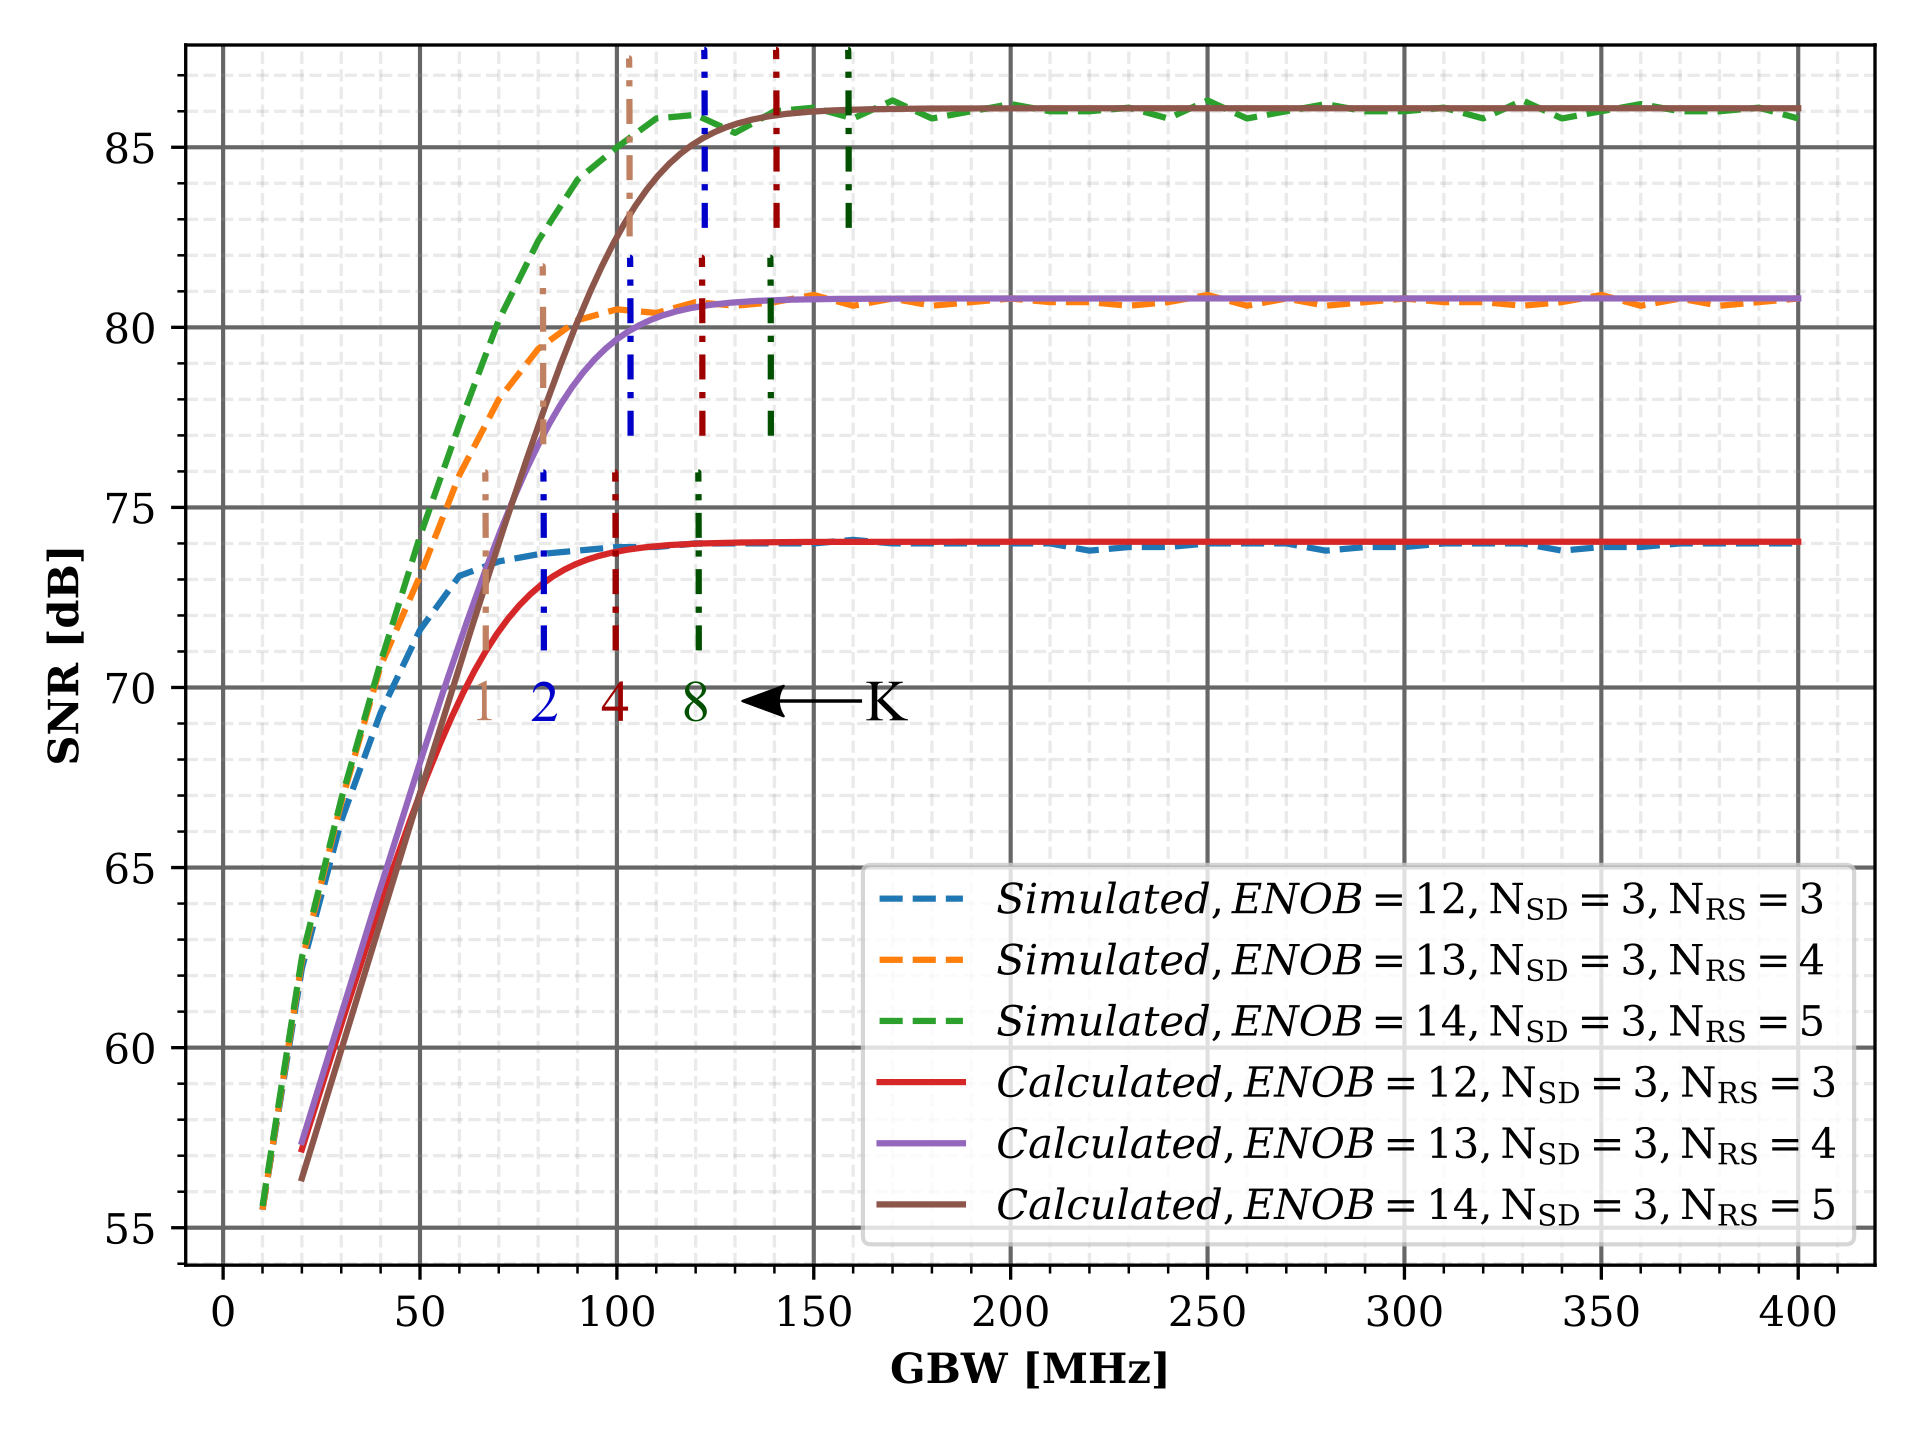
\includegraphics[scale=.7]{Chap04/Figures/snr_vs_gbw_calc1.png}
    \caption{Comparison between the simulated and modeled SNR equation w.r.t. GBW}
    \label{fig:SNR_GBW_calc1}
\end{figure}


In order to verify how closely the above equation represents the simulated curve, the graphs are plotted using the eq(\ref{ERR_RMS_GBW}) by varying the GBW, along with simulated graphs as shown in fig(\ref{fig:SNR_GBW_calc}). Three cases of ENOB of 12, 13 and 14 are considered keeping the resolution in IADC constant (3-bit) and RADC resolution of 3, 4 and 5-bit. The dotted characteristics represents simulated curves while the solid ones are plotted using eq.(\ref{ERR_RMS_GBW}). Both graphs (simulated and modeled) are reasonably immediate to each other. When the simulated characteristic reaches it's maximum, the modeled one is hardly farther by 2~dB. For example, the case with $N_{RS}=5$, simulated (dotted green) characteristic attains it's maximum value of 86~dB at GBW of 115~dB, while modeled characteristic has an SNR value of 85~dB.

Now, as a next step, we need to find the value of GBW, such that the error on the residue due to GBW is much smaller than the overall quantization noise of ERADC i.e. eq(\ref{COMP_ERR}) holds. Then, let's assume a factor $K$ such a that,

\begin{align*}
    Error_{e[M]_{rms}} = \frac{Q_{eradc_{rms}}}{K}
\end{align*}

Where $K$ is large enough to hold the eq(\ref{COMP_ERR}). Then, putting the values of eq(\ref{ERR_RMS_GBW}) and (\ref{QN_ERADC}) in the equation above,

 \begin{equation*}
    \frac{1}{\sqrt{3}}\frac{2}{M(M-1)}\frac{V_{ref}}{\left(2^{N_{SD}}-1\right)}e^{-\left(\frac{\pi GBW}{F_s}\right)}  = \frac{1}{2\sqrt{3}K}\frac{2}{M(M-1)}\frac{V_{ref}}{\left(2^{N_{SD}}-1\right)\left(2^{N_{RS}}-1\right)}
\end{equation*}

 \begin{equation*}
    e^{-\left(\frac{\pi GBW}{F_s}\right)}  = \frac{1}{2K\left(2^{N_{RS}}-1\right)}
\end{equation*}

 \begin{equation*}
    e^{\left(\frac{\pi GBW}{F_s}\right)}  = 2K\left(2^{N_{RS}}-1\right)
\end{equation*}

\begin{equation}\label{eq:GBW}
    GBW = \frac{F_s}{\pi} \ln{\left[2K\left(2^{N_{RS}}-1\right)\right]}
\end{equation}

\begin{table}[]
\centering
\resizebox{\textwidth}{!}{
% Please add the following required packages to your document preamble:
% \usepackage{multirow}
\begin{tabular}{c|c|c|c|c|c|c|c|c|c|c|c|c}
\Xhline{5\arrayrulewidth}
\multirow{2}{*}{\textbf{N\textsubscript{RS}}} & \multicolumn{3}{c|}{\textbf{K=1}}       & \multicolumn{3}{c|}{\textbf{K=2}}       & \multicolumn{3}{c|}{\textbf{K=4}}       & \multicolumn{3}{c}{\textbf{K=8}}       \\ \cline{2-13} 
                     & \textbf{GBW}  & \textbf{SNR\textsubscript{sim}} & \textbf{SNR\textsubscript{calc}} & \textbf{GBW}  & \textbf{SNR\textsubscript{sim}} & \textbf{SNR\textsubscript{calc}} & \textbf{GBW}  & \textbf{SNR\textsubscript{sim}} & \textbf{SNR\textsubscript{calc}} & \textbf{GBW}  & \textbf{SNR\textsubscript{sim}} & \textbf{SNR\textsubscript{calc}} \\ \hline
3                    & 67  & 73.5      & 71       & 85  & 73.9      & 73.1       & 102.5 & 74        & 74       & 120 & 74        & 74         \\ \hline
4                    & 80  & 79.5      & 77       & 103 & 80.3      & 79.9       & 122   & 80.8      & 80.8     & 139 & 80.8        & 80.8       \\ \hline
5                    & 104 & 85.1      & 83       & 123 & 85.8      & 85.3       & 140   & 86        & 86       & 160 & 86        & 86       \\ \Xhline{5\arrayrulewidth}
\end{tabular}
}
\caption{Comparison between the Simulated SNR and the SNR on the modeled characteristic (in dB) for different values of $K$ as a function of calculated Finite GBW (in MHz)}
\label{SIM_CALC_COMP_GBW}
\end{table}


Tab. \ref{SIM_CALC_COMP_GBW} shows the comparison between the simulated SNR and the SNR on the modeled characteristic for different values of $K$ as a function of calculated Finite GBW using eq (\ref{eq:GBW}). For $K=1$, the value of the on the modeled characteristic is 3~dB down the maximum SNR, however, the difference w.r.t. simulated one is less than 2~dB. As $K$ goes on increasing, the calculated values of SNR closely represents the simulated ones, furthermore $K=4$ and $K=8$ results in the equal values of simulated and calculated values.


\subsubsection{GBW of the First-Integrator Op-Amp}
The performance of standalone IADC and extended-range IADC as a function of the first-integrator op-amp GBW is shown in Fig. \ref{SNR_GBW1}. Considering an ENOB requirement of 14 bit (SNR of 86~dB), the standalone IADC requires 60~MHz of GBW with a conversion time of 90 clock cycles, while the extended a conversion time of merely 18 clock cycles.
\begin{figure}[h]
\centering
\subfigure[]{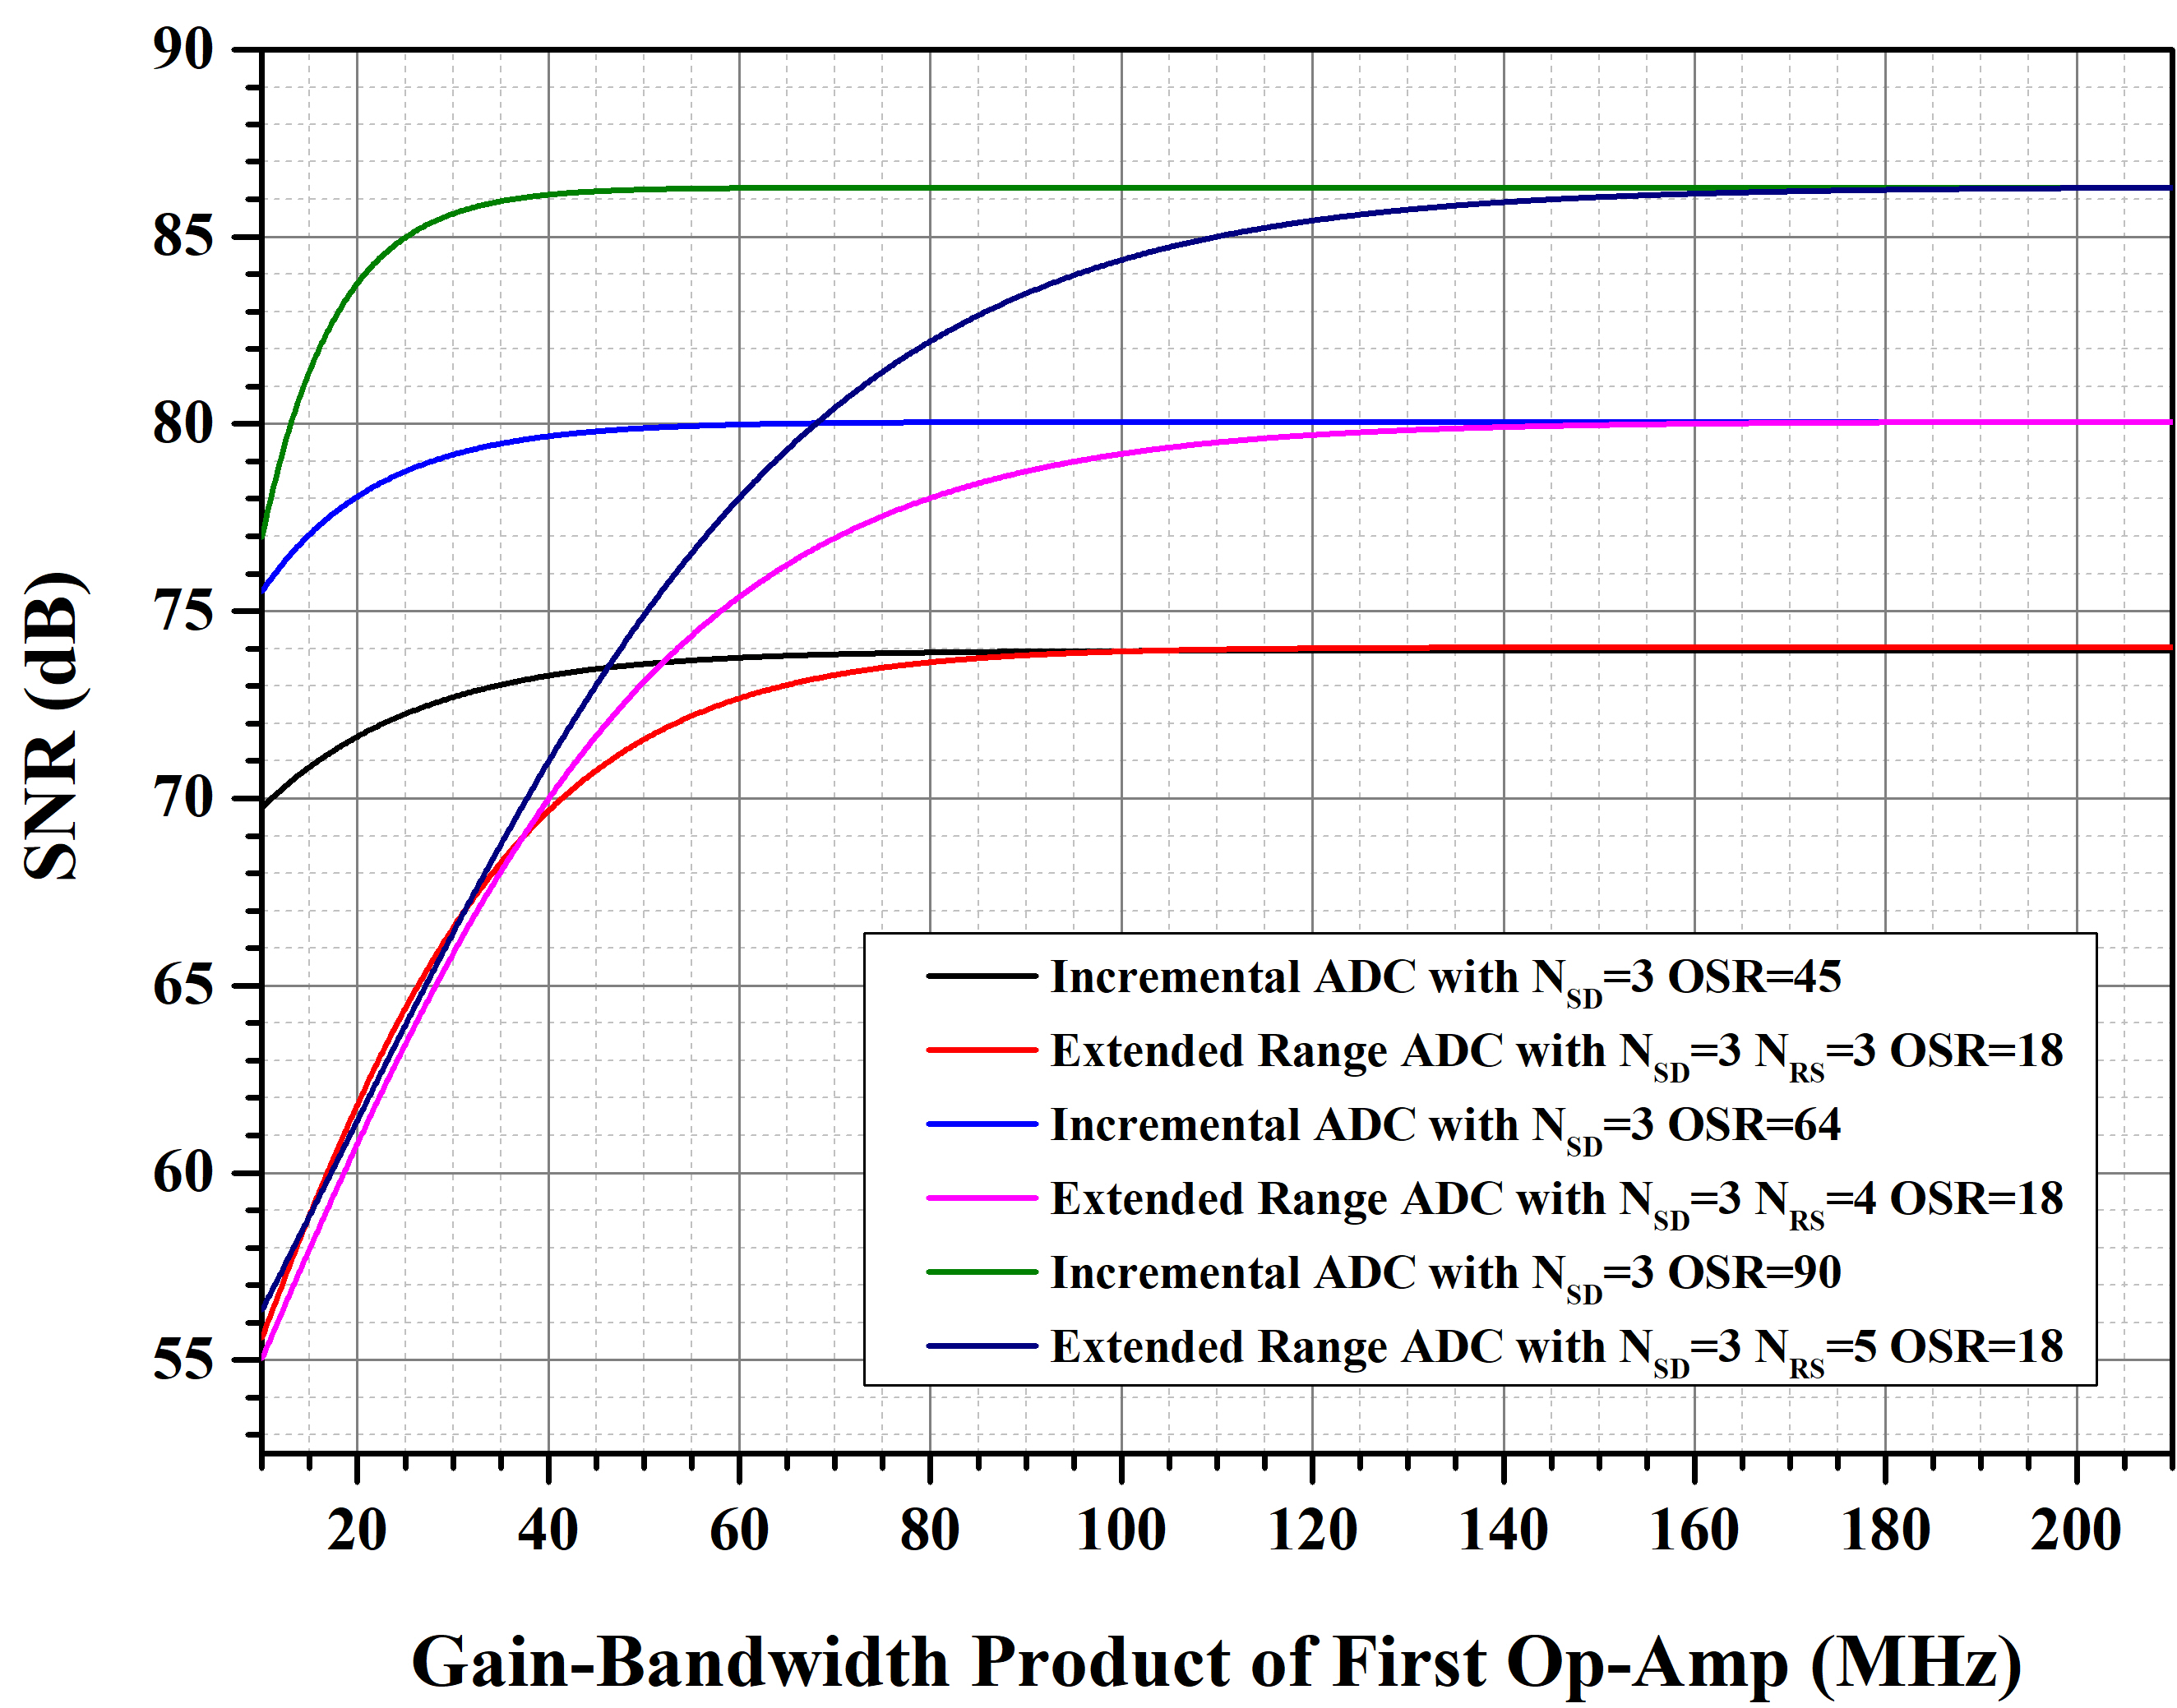
\includegraphics[scale=.28]{Chap04/Figures/SNR_GBW1_NSD3}}
\qquad
\subfigure[]{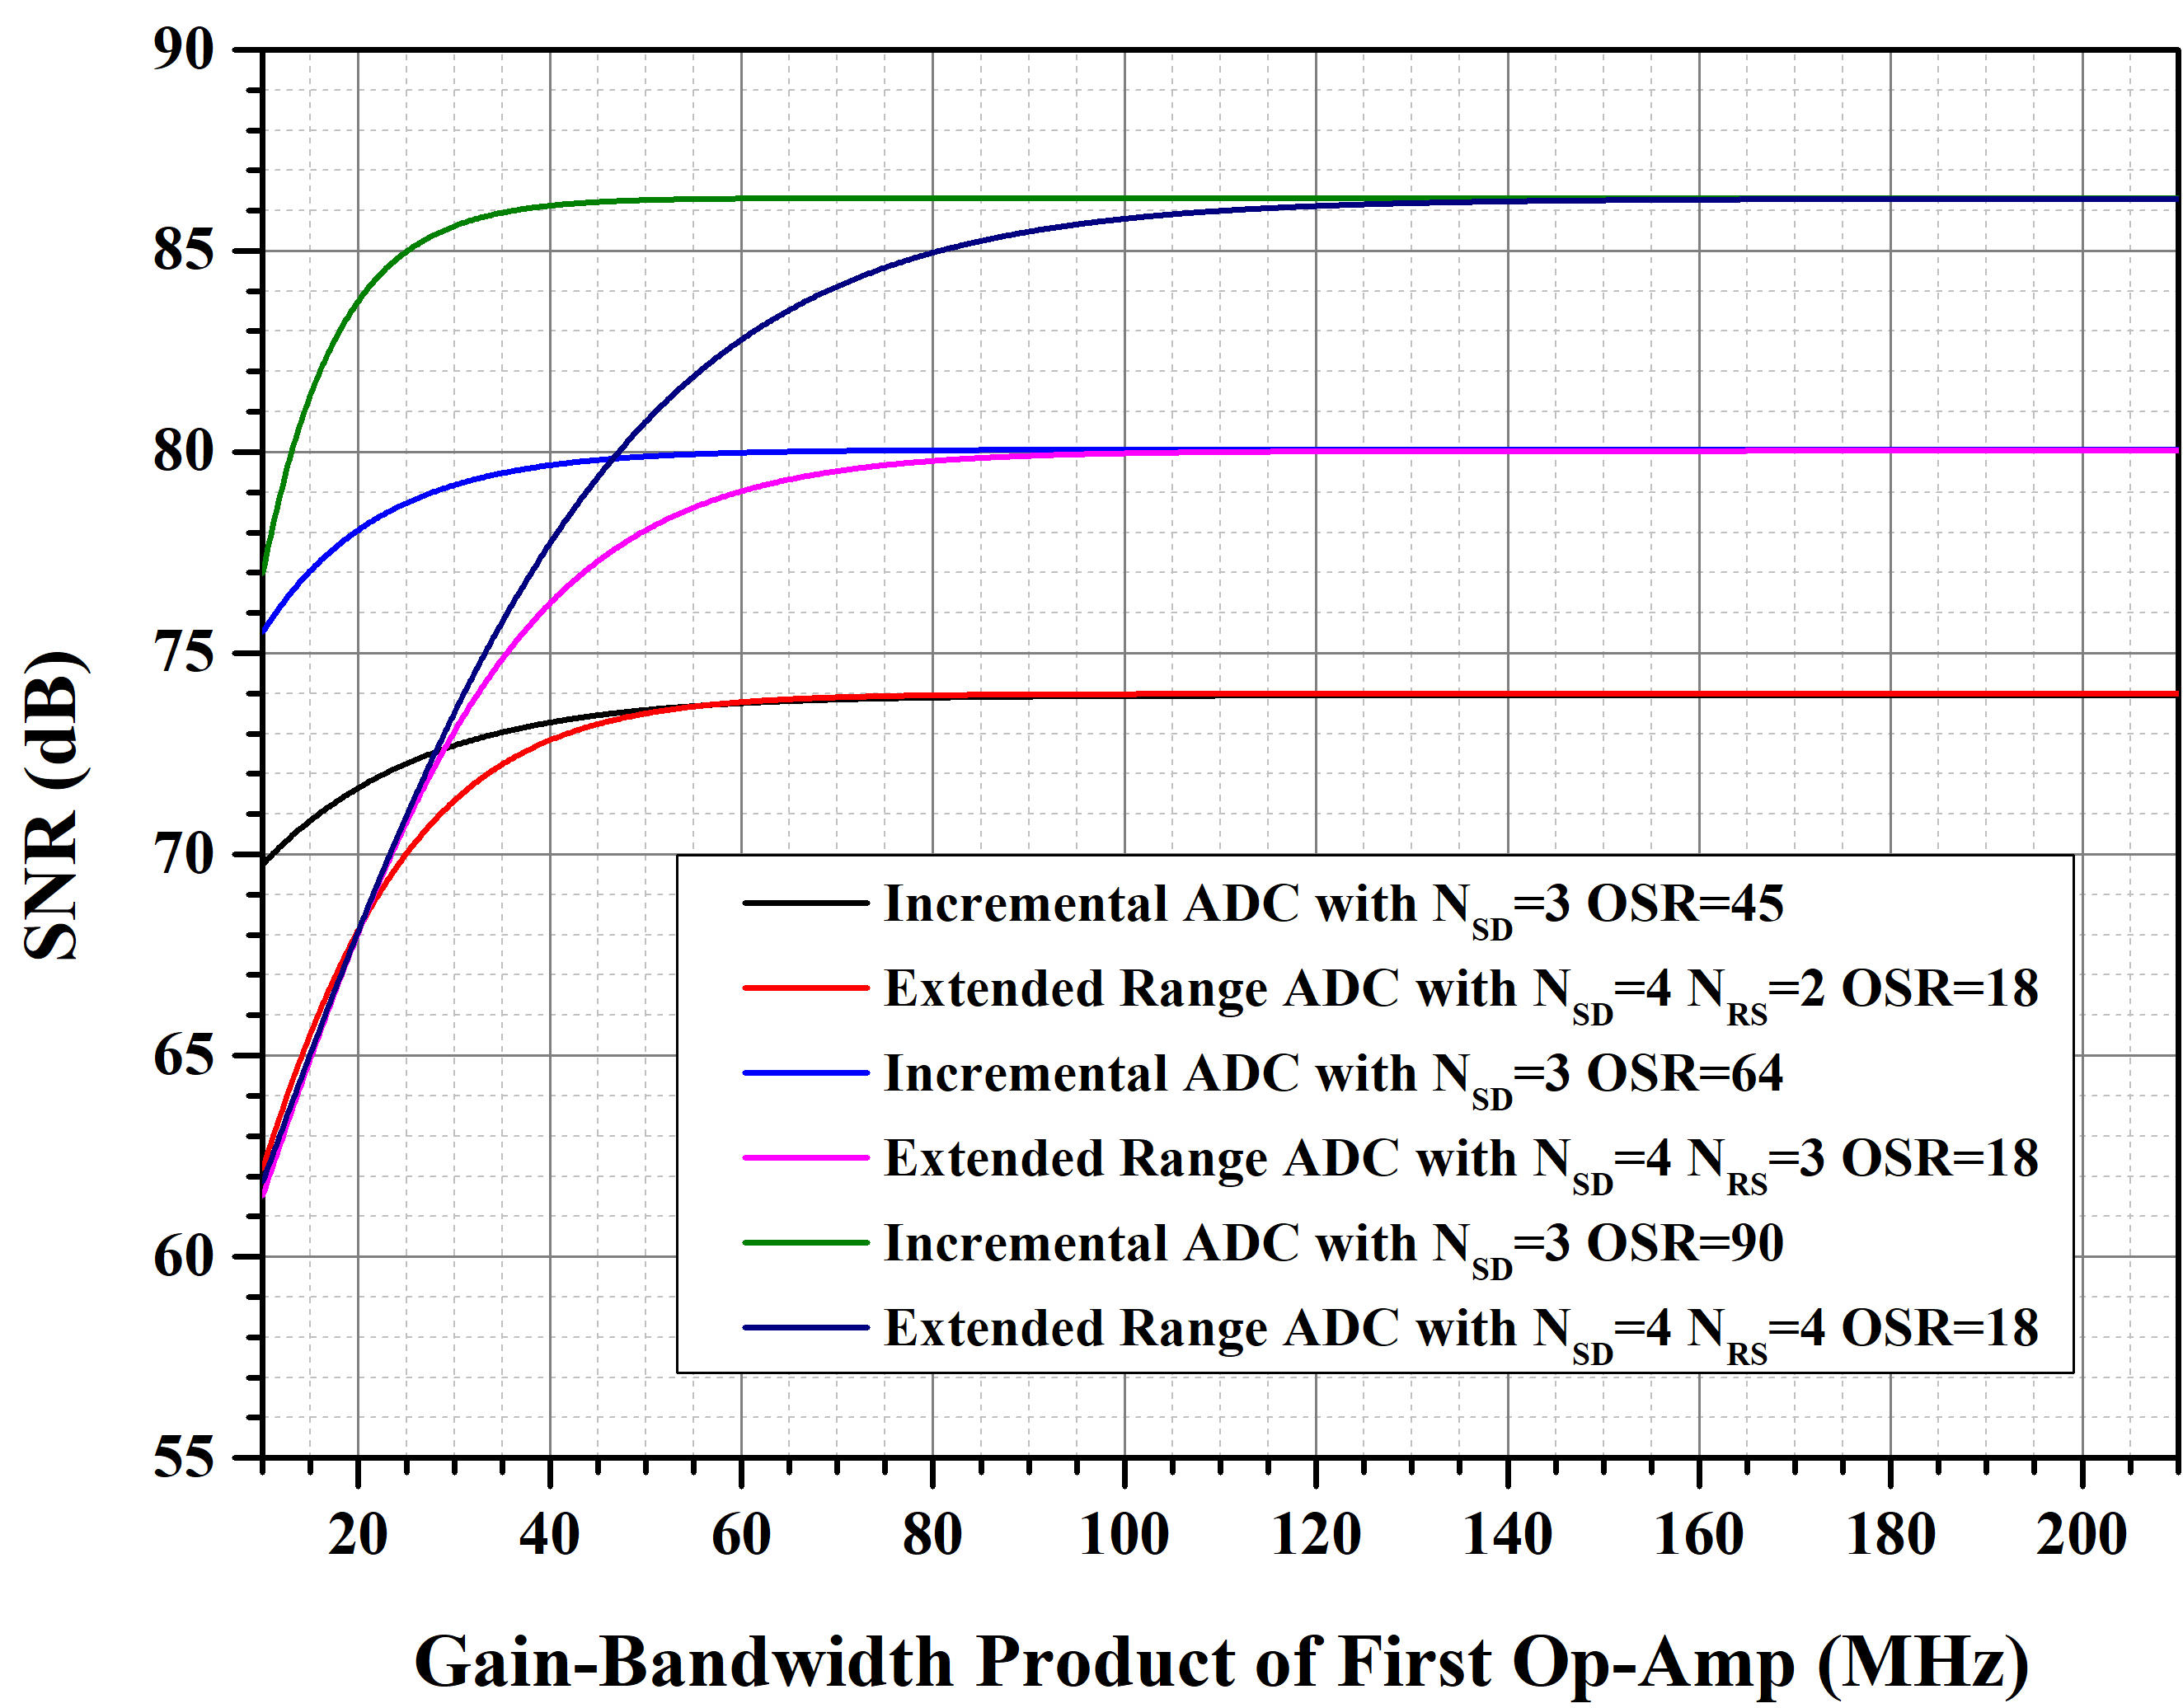
\includegraphics[scale=.28]{Chap04/Figures/SNR_GBW1_NSD4}}
\caption{Comparison of the IADC and extended-range IADC with different values of the first-integrator op-amp GBW}
\label{SNR_GBW1}
\end{figure}

\subsubsection{GBW of the Second-Integrator Op-Amp}
The second-integrator op-amp GBW has a negligible effect on the performance of a standalone IADC, but again it affects the overall performance of extended-range IADCs, as shown in Fig. \ref{SNR_GBW2}. For an ENOB of 14 bit, the standalone IADC needs 40~MHz of GBW, while the extended-range IADC with $N_{INC}=9$ and $N_{RS}=5$ requires a GBW of 160~MHz.
\begin{figure}[h]
\centering
\subfigure[]{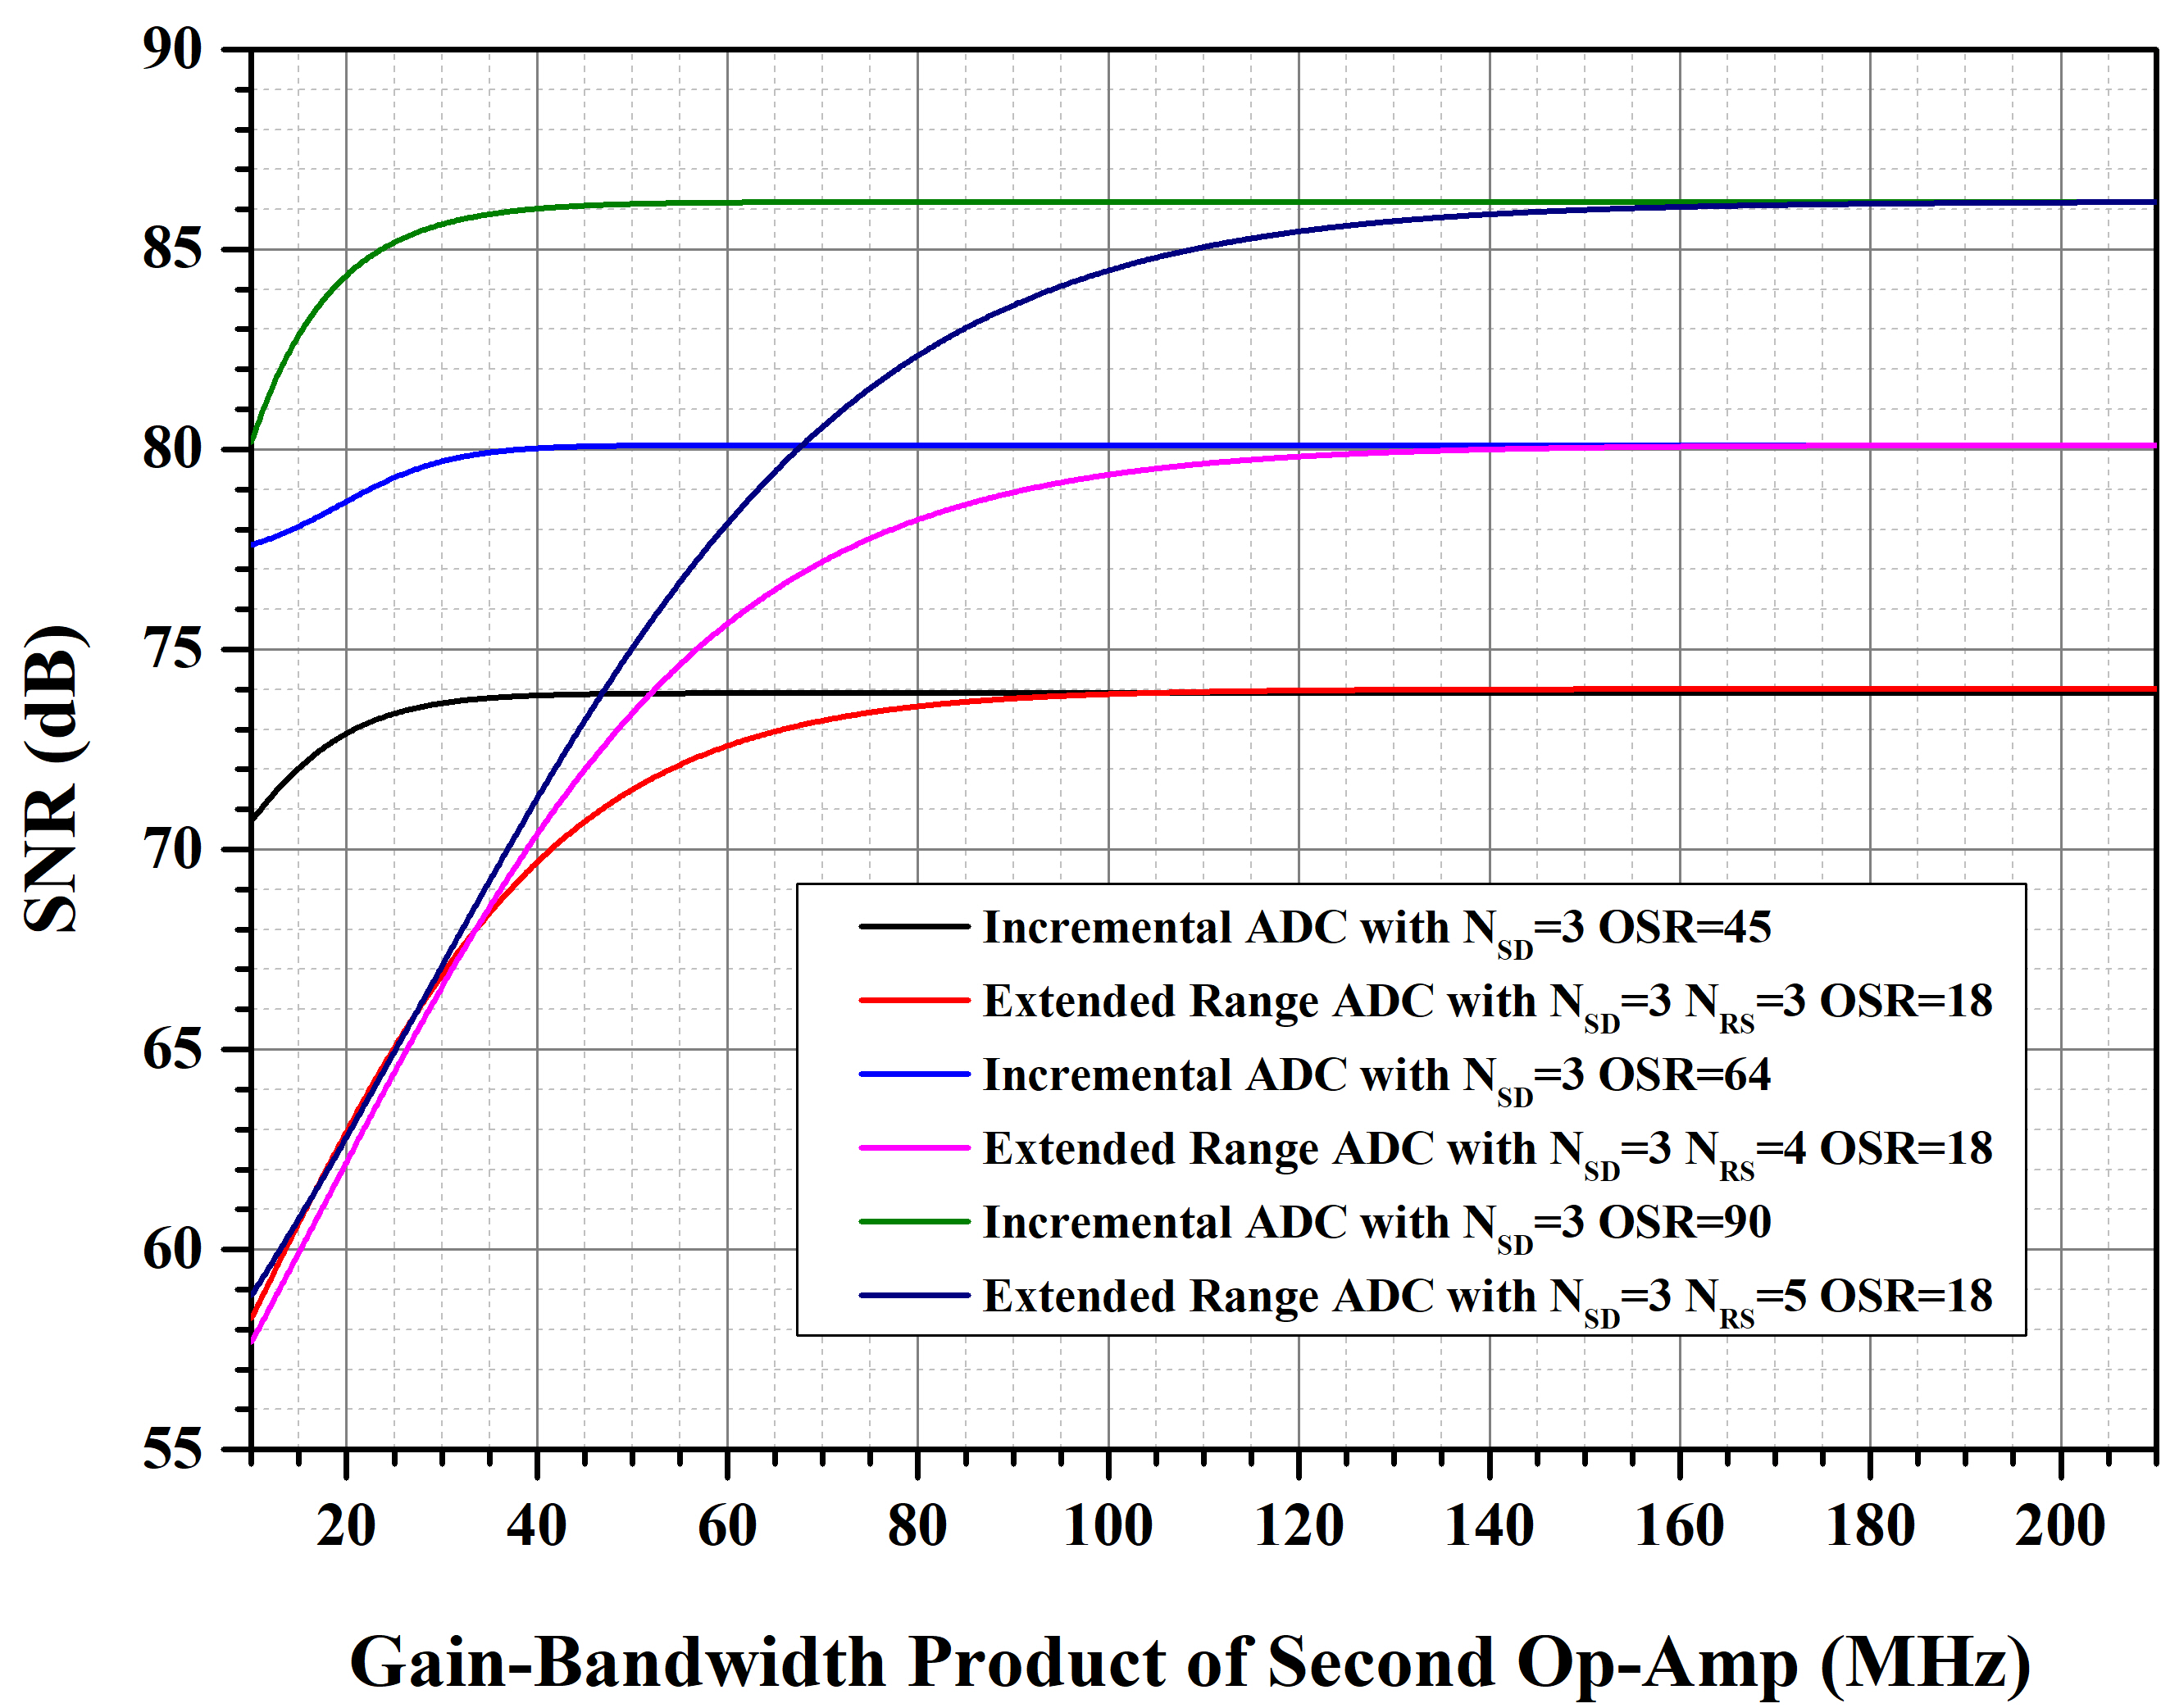
\includegraphics[scale=.28]{Chap04/Figures/SNR_GBW2_NSD3}}
\qquad
\subfigure[]{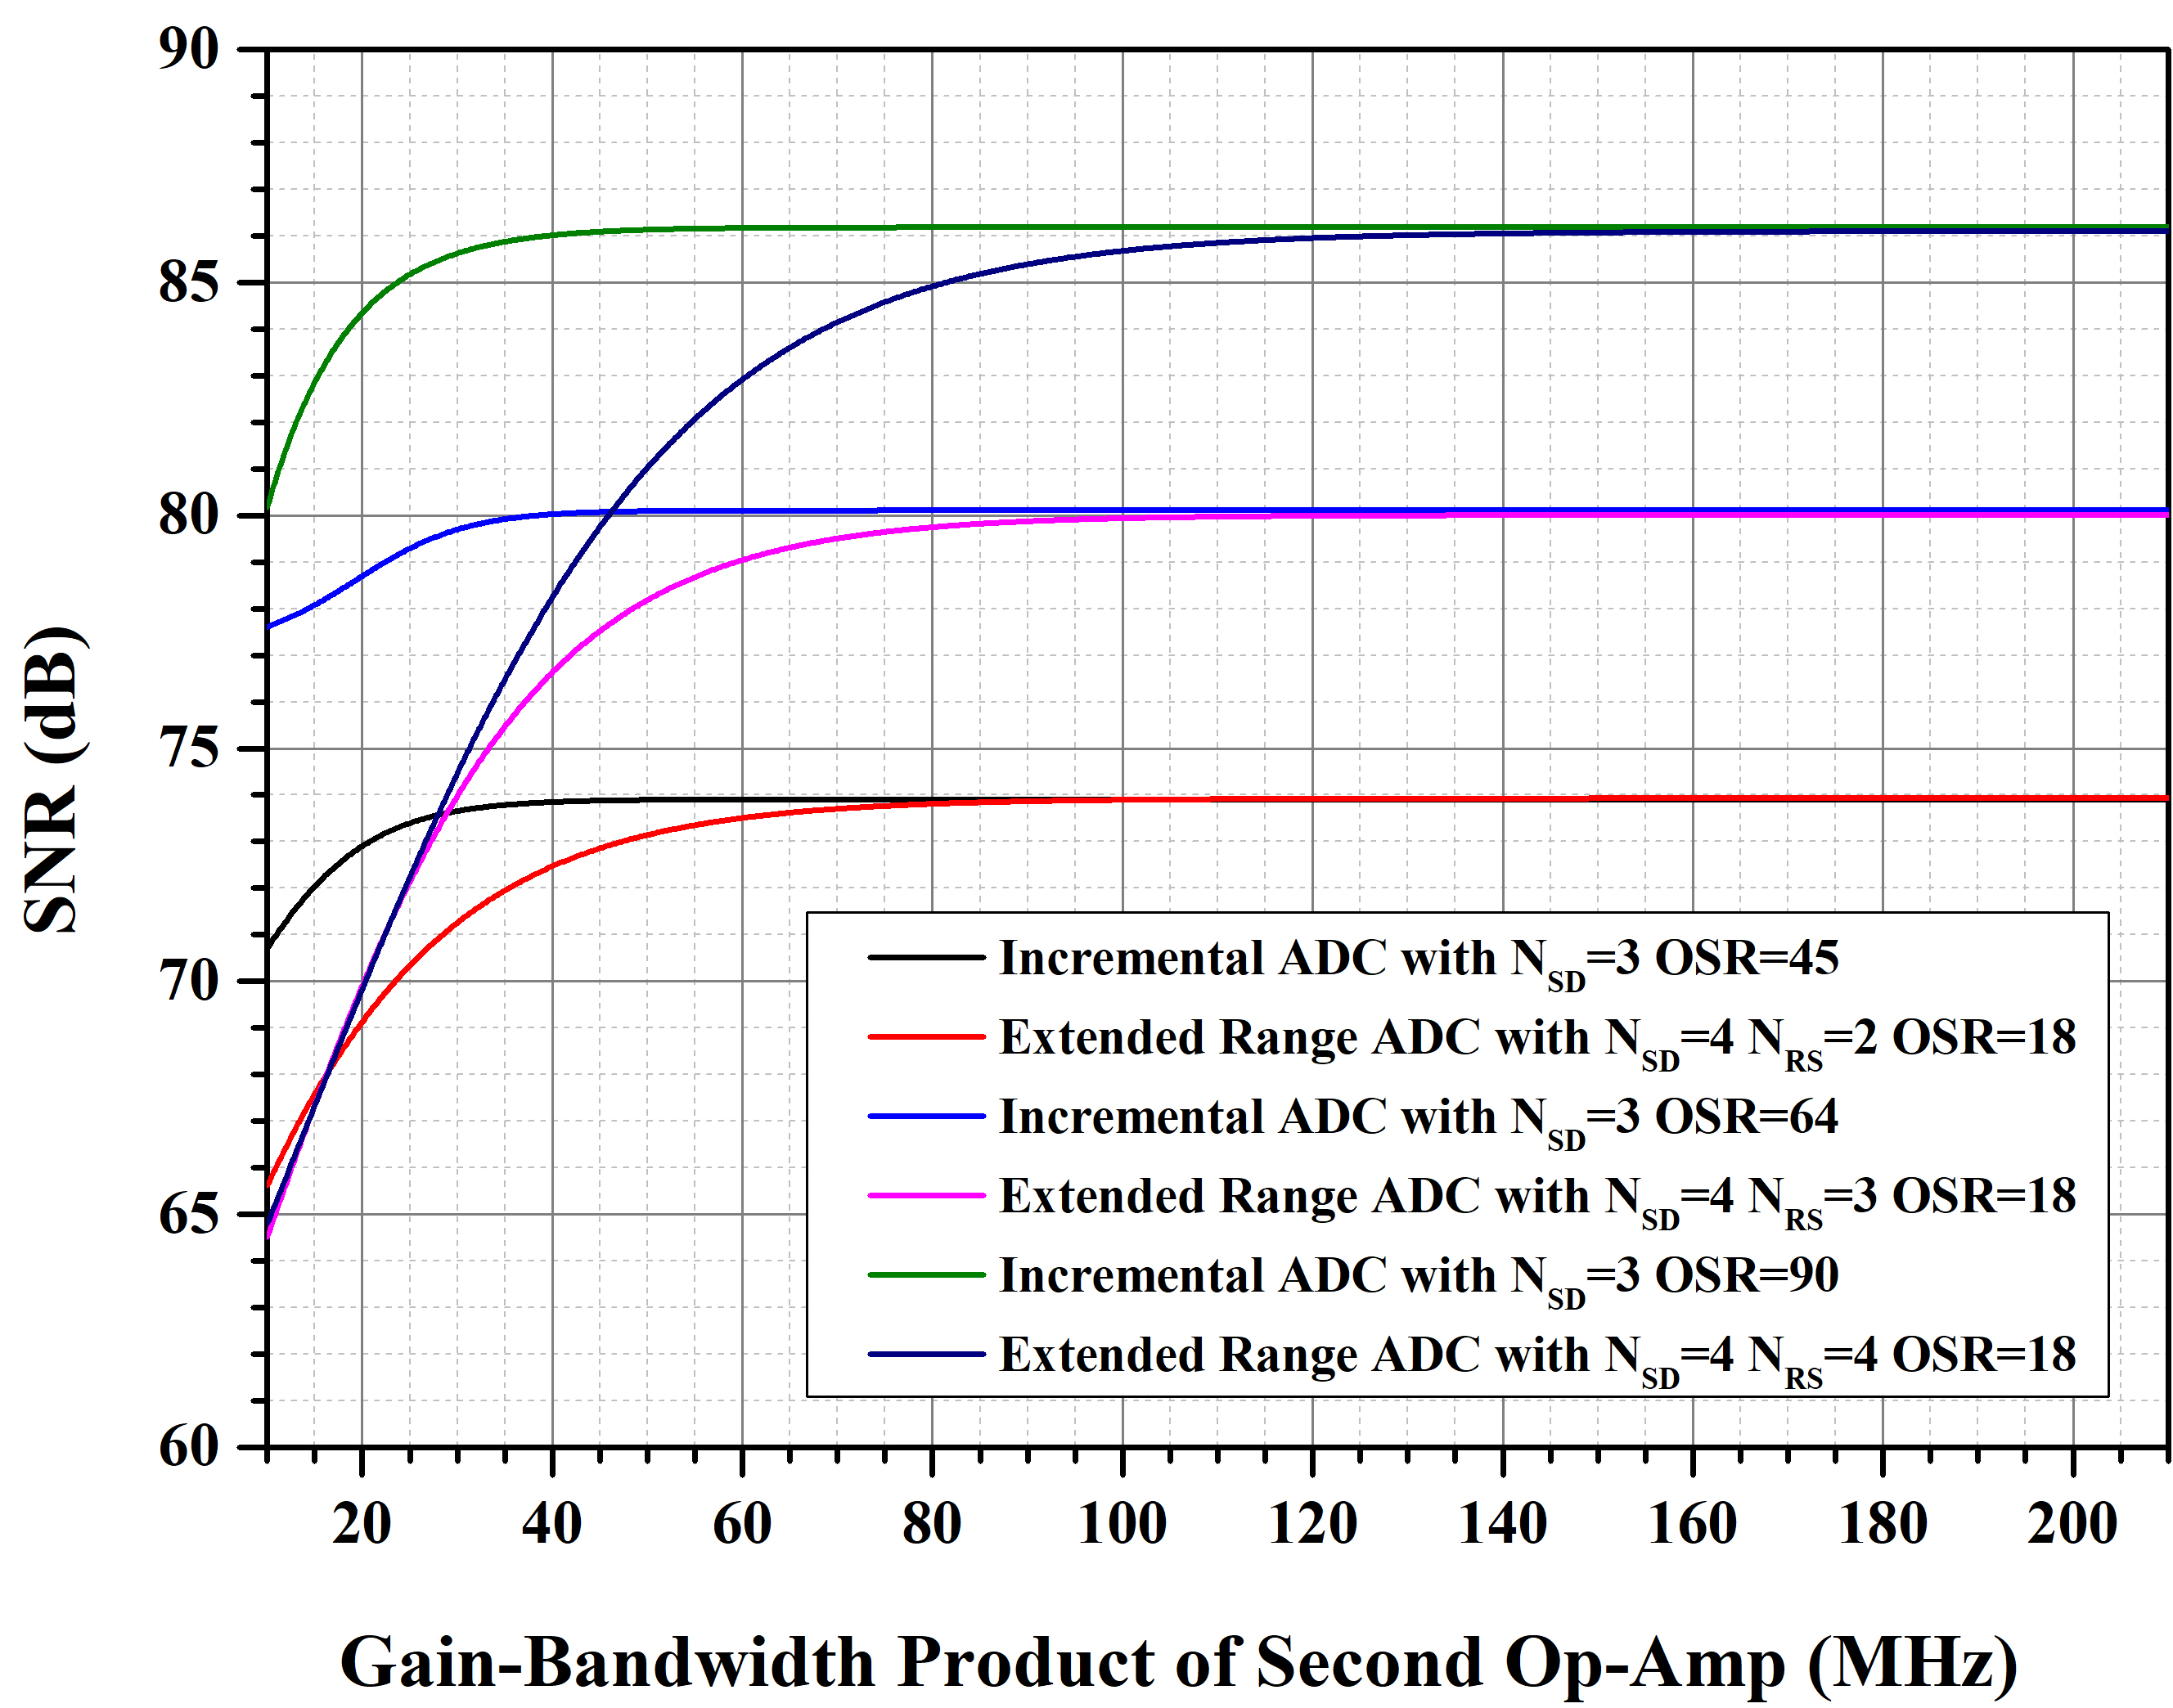
\includegraphics[scale=.28]{Chap04/Figures/SNR_GBW2_NSD4}}
\caption{Comparison of the IADC and extended-range IADC with different values of the second-integrator op-amp GBW}
\label{SNR_GBW2}
\end{figure}


\subsection{Performance Comparison}
The results of the analysis of the effect of op-amp gain and GBW on the ADC performance are summarized in Tab.~\ref{COMPARISON}. Basically, it turns out that, by adding extended range to an IADCs, the strong reduction of the conversion time for the same ENOB is achieved at the expense of tougher op-amp gain and GBW specifications.
\begin{table}[h]
\centering
% \resizebox{\textwidth}{!}{
\begin{tabular}{c|c|c|c|c|c|c|c|c|c}
\Xhline{4\arrayrulewidth}
\textbf{ENOB\textsubscript{TOT}} & \multicolumn{3}{c|}{\textbf{12}} & \multicolumn{3}{c|}{\textbf{13}} & \multicolumn{3}{c}{\textbf{14}} \\ \hline
\textbf{N\textsubscript{SD}} & 3 & 3 & 4 & 3 & 3 & 4 & 3 & 3 & 4 \\ \hline
\textbf{ENOB\textsubscript{INC}} & 12 & 9 & 10 & 13 & 9 & 10 & 14 & 9 & 10 \\ \hline
\textbf{N\textsubscript{RS}} & 0 & 3 & 2 & 0 & 4 & 3 & 0 & 5 & 4 \\ \hline
\textbf{OSR} & 45 & 18 & 18 & 64 & 18 & 18 & 90 & 18 & 18 \\ \hline
\textbf{Gain1 (dB)} & 36 & 58 & 50 & 38 & 76 & 70 & 40 & 80 & 80 \\ \hline
\textbf{Gain2 (dB)} & 36 & 58 & 52 & 38 & 74 & 60 & 40 & 80 & 70 \\ \hline
\textbf{GBW1 (MHz)} & 60 & 110 & 80 & 60 & 150 & 100 & 60 & 190 & 150 \\ \hline
\textbf{GBW2 (MHz)} & 40 & 90 & 80 & 40 & 130 & 90 & 40 & 160 & 130 \\ \Xhline{4\arrayrulewidth}
\end{tabular}
% }
\caption{Comparison of the op-amp requirements for standalone IADC and extended-range IADC}
\label{COMPARISON}
\end{table}


The extended-range IADC with 3-bit quantizer and $N_{RS}=5$ requires 18 clock cycles per conversion to achieve 86~dB of SNR (14-bit ENOB). The same ENOB can also be achieved with 4-bit quantizer and $N_{RS}=4$ still requiring 18 clock cycles. However, it is clear that the sensitivity to op-amp non-idealities is different in the two cases. The ADC with $N_{RS}=5$ require a gain in both op-amps of 80~dB, a GBW in first-integrator op-amp of 190~MHz and a GBW in the second-integrator op-amp of 160~MHz, while the ADC with $N_{RS}=4$ requires more relaxed op-amp specifications (gain of 80~dB and GBW of 150~MHz, gain of 70~dB and GBW of 130~MHz in the two op-amps, respectively). This is due to the fact that a higher resolution in the ERADC requires higher accuracy in the residue value. However, the 4-bit IADC quantizer of the ADC with $N_{RS}=4$ is twice as large and power hungry than the 3-bit quantizer of the ADC with $N_{RS}=5$.


%%%%%%%%%%%%%%%%%%%%%%%%%%%%%%%%%%%%%%%%%%%%%%%%%%%%%%%%%%%%%%%%%%%%%%%%%%%%%%%%%%%%%%%%%%%%%%%%%%%%%%%%%%%%%%%%%%%%
%%%%%%%%%%%%%%%%%%%%%%%%%%%%%%%%%%%%%%%%%%%%%%%%%%%%%%%%%%%%%%%%%%%%%%%%%%%%%%%%%%%%%%%%%%%%%%%%%%%%%%%%%%%%%%%%%%%%
% \section{Selection of the Extended-Range ADC Architecture:}

% Every increase of a bit in the quantizer resolution doubles the number of comparators in it exhibiting an exponential rise. The comparators required for 3-bit flash are 7 while that for 4-bit are 15. Certainly the case with 15 comparators becomes much more complicated. Therefore, for the further analysis and implementation, instead of the two cases of $N_{SD} = 3$ and $N_{SD} = 4$, a lower resolution cases in the IADC quantizer i.e. $N_{SD} = 2$ and $N_{SD} = 3$ are considered which saves the significant amount of power and the implementation also becomes quite simple.

% So far, the general analysis of the op-amp requirements is carried out which yielded the expressions for the non-idealities such as Low Frequency Gain and Gain-Bandwidth Product. Now the all the requirements such as Gain, GBW, resolutions to be considered etc. is available for further analysis such as capacitor mismatch.

% A complete model of the Incremental {\textSigma}{\textDelta} Modulator with extended counting (Extended Range Incremental {\textSigma}{\textDelta} Modulator) is developed in the simulink as shown in Fig. \ref{SIM_ERISDM}.  Various permutations and combinations of the resolutions of the I{\textSigma}{\textDelta}M and Residual ADC are verified for given clock frequency of 80 MHz, total conversion time of 25 clock cycles to attain digitization accuracy of 74 dB SNR but additional 12 dB margin to accommodate also the process corners' degradation, combining which to the required SNR makes it 86 dB. Therefore the model is structured in a fashion so that ideally it should exhibit overall SNR of 86 dB or ENOB of 12. 

% However, the capacitor mismatch in the integrator can modify its coefficient from its nominal value which could significantly affect the overall performance.


% % \begin{itemize}
% %     \item{\makebox[5cm][l]{I{\textSigma}{\textDelta}M Resolution = 2} Residual ADC Resolution = 5}
% %     \item{\makebox[5cm][l]{I{\textSigma}{\textDelta}M Resolution = 2} Residual ADC Resolution = 6}
% %     \item{\makebox[5cm][l]{I{\textSigma}{\textDelta}M Resolution = 2} Residual ADC Resolution = 7}
% %     \item{\makebox[5cm][l]{I{\textSigma}{\textDelta}M Resolution = 3} Residual ADC Resolution = 3}
% %     \item{\makebox[5cm][l]{I{\textSigma}{\textDelta}M Resolution = 3} Residual ADC Resolution = 4}
% %     \item{\makebox[5cm][l]{I{\textSigma}{\textDelta}M Resolution = 3} Residual ADC Resolution = 5}
% % \end{itemize}

% \subsection{For I{\textSigma}{\textDelta}M Resolution of 2:}
% The effect of finite gain of the op-amps on the overall performance of the modulator has been studied considering the 2-bit of resolution of the quantizer in I{\textSigma}{\textDelta}M while the resolution of the residual ADC is varied as shown in the Fig. \ref{SNR_GAIN_NSD2} and the rest of the parameters are kept ideal. It is explicit from the figure that the least magnitude of the gain of the op-amps to sustain a maximum SNR is 60 dB, below which the performance degrades to the significant extent.

% To study the dependence of the overall Gain-Bandwidth Product (GBW) of the first Op-Amp over the SNR, all the other parameters, including the Gain, are brought back to the ideal values and GBW of the first Op-Amp is varied from 30 MHz to 300 MHz as shown in Fig. \ref{GBW_Vs_SNR_NSD2}(a). To achieve the maximal stable SNR, the promising value of the GBW of the first op-amp could be 250 MHz. Similar procedure is followed to observe the effect of GBW of second op-amp on the comprehensive SNR and the response is plotted as shown in the Fig.\ref{GBW_Vs_SNR_NSD2}(b).

% Another crucial non-ideality to be examined is the slew rate (SR). The SR of the first op-amp (Fig. \ref{SR_Vs_SNR_NSD2}(a)) and the second op-amp (Fig. \ref{SR_Vs_SNR_NSD2}(b)) are altered from maximum ideal value to certain minimum value and responses are plotted. For the purpose to meet the maximum SNR, the requirement of SR of first op-amp is 270 $V/\mu s$ and that of the second op-amp is found to be 170 $V/\mu s$.

% The next issue which needs to be studied is the capacitor ratio mismatch in the integrators which forms the required coefficient. The variation in the capacitors from their mean value in the switched capacitor integrator changes the integrator coefficient which leads to the performance deterioration. Fig. \ref{CAPMIS_Vs_SNR_NSD2} shows the graphs where the overall SNDR is plotted against capacitor mismatch for both of the integrators. It is explicit from these plots that the SNDR attains maximum value when the mismatch is 0\% and degrades for increasing or decreasing value of the coefficient.
% \begin{figure}[h]
% \centering
% 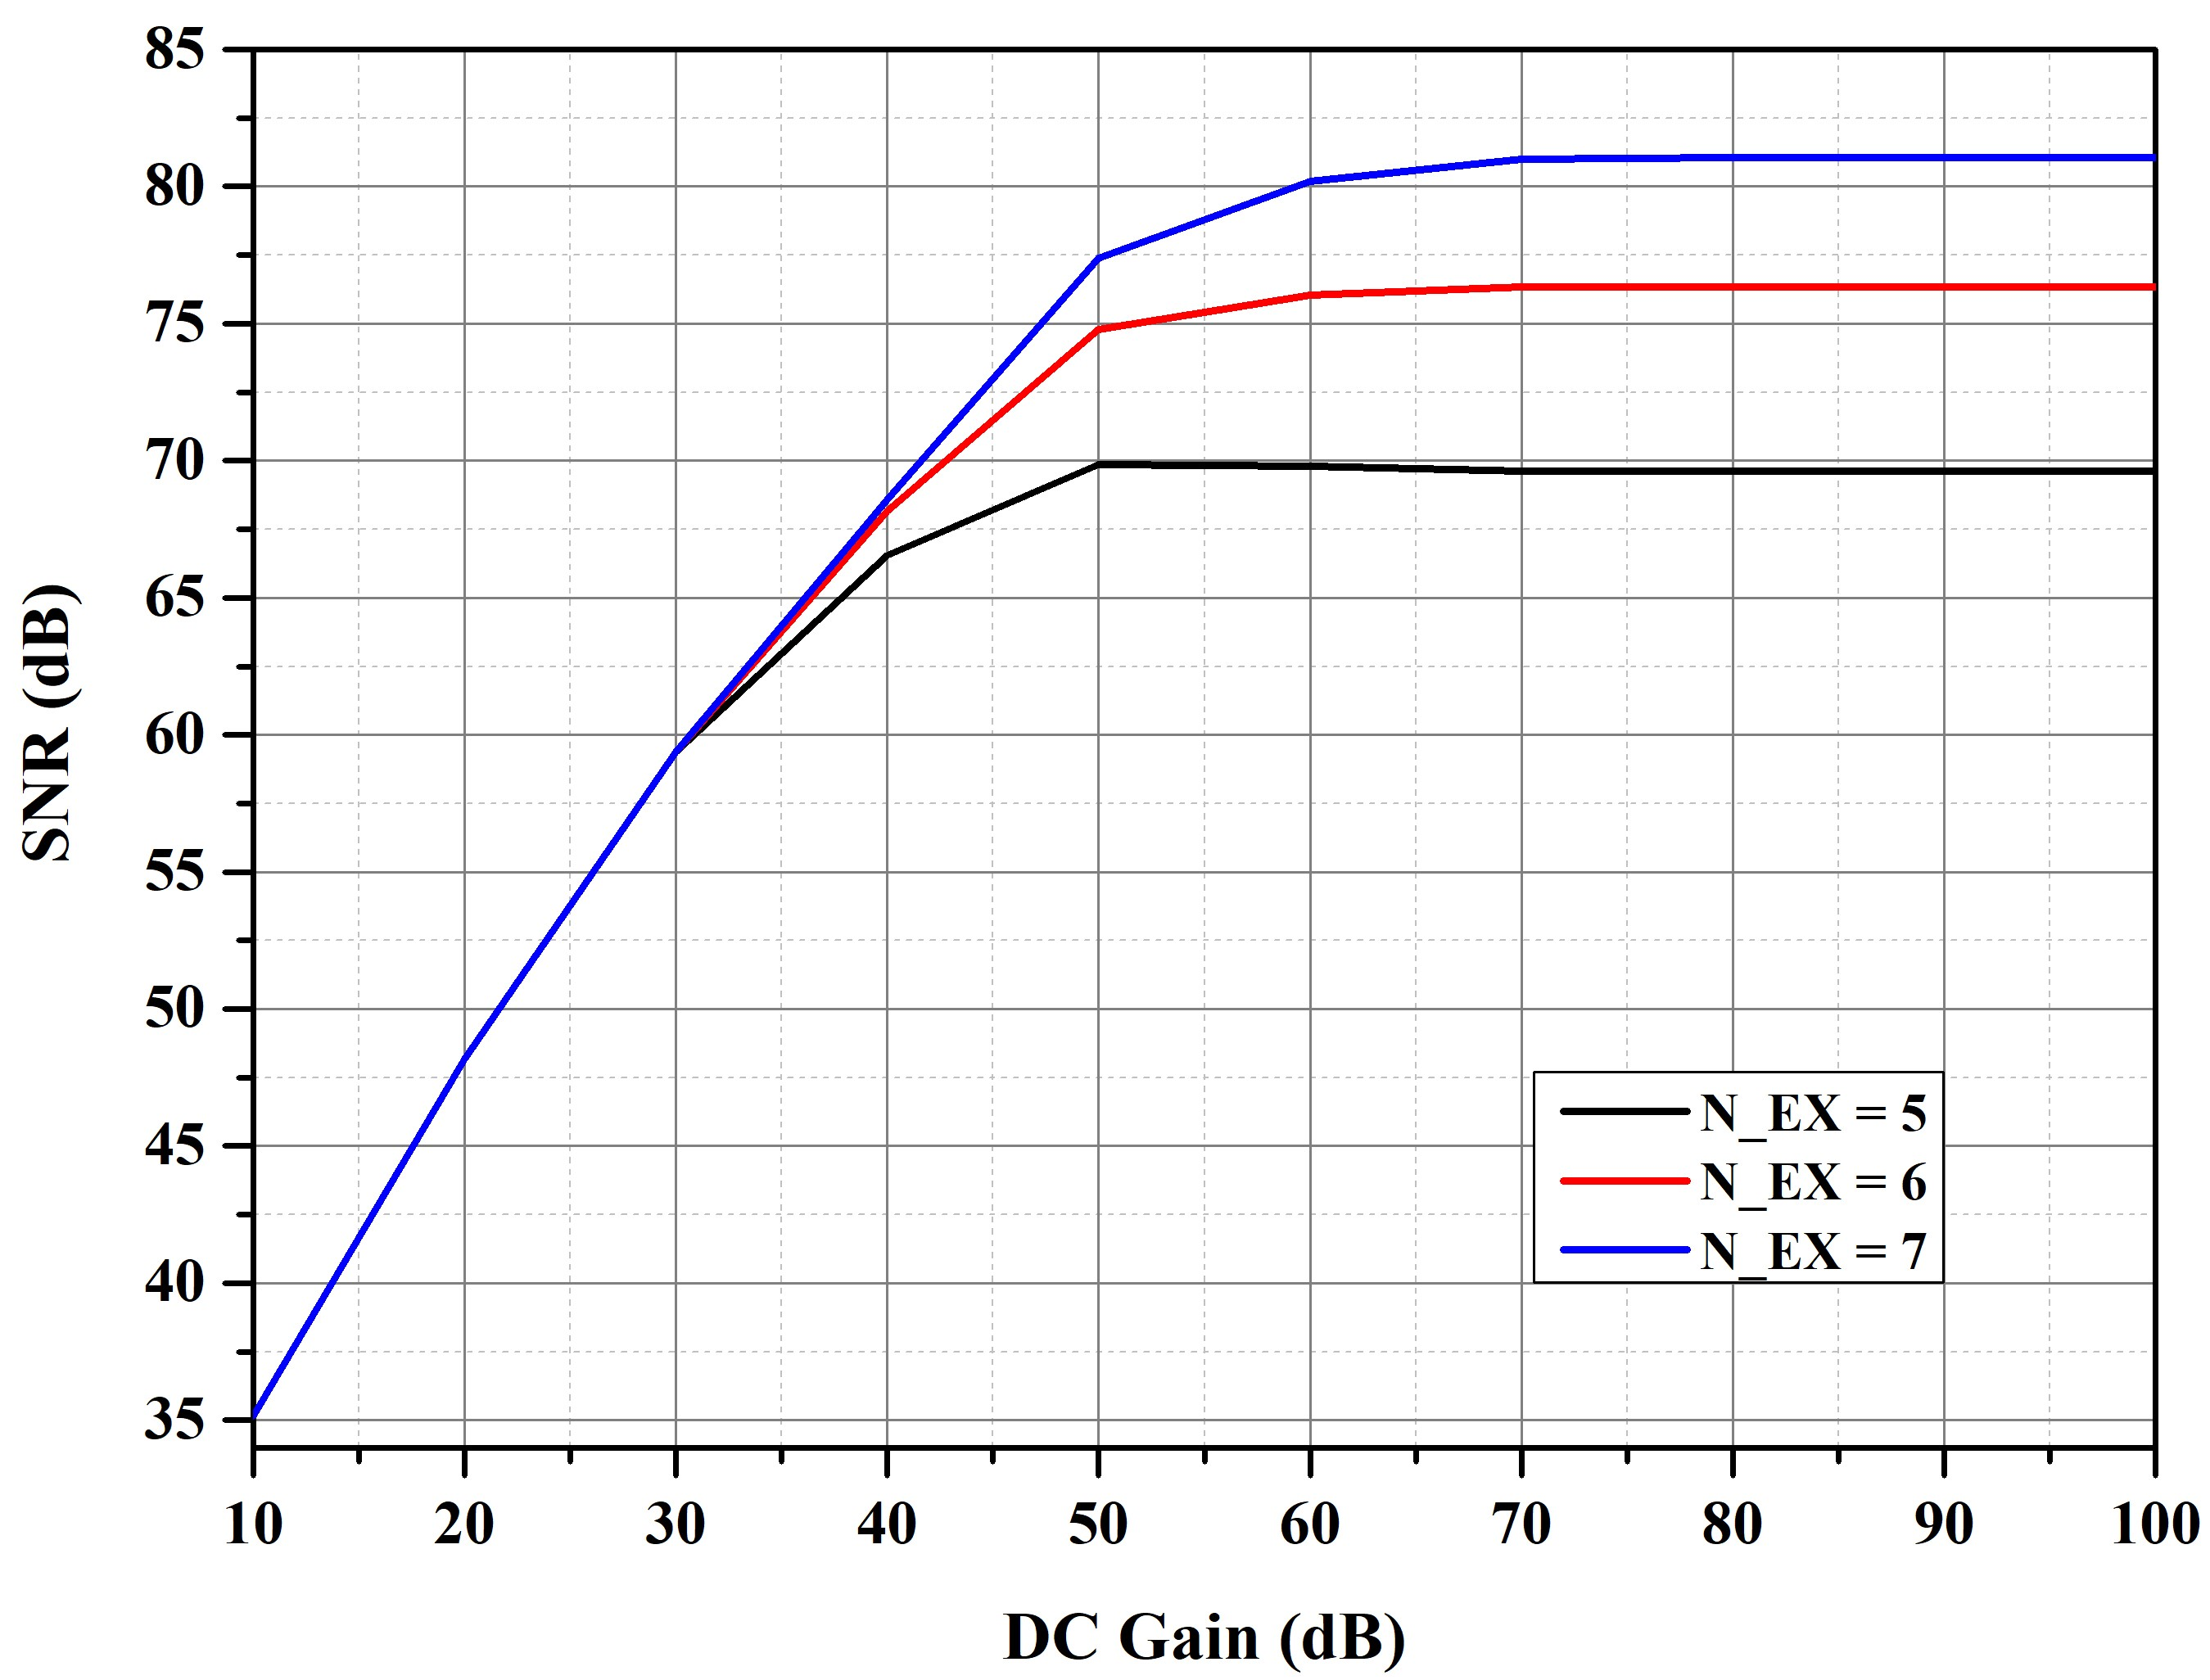
\includegraphics[width=0.5\columnwidth]{Chap04/Figures/snr_vs_gain_nsd2.jpg}
% \caption{Gain of the Op-Amps Vs Overall SNR of the Extended Counting Incremental {\textSigma}{\textDelta} Modulator}
% \label{SNR_GAIN_NSD2}
% \end{figure}


% \begin{figure}[h]
%     \centering
%     \subfigure[]
%     {
%         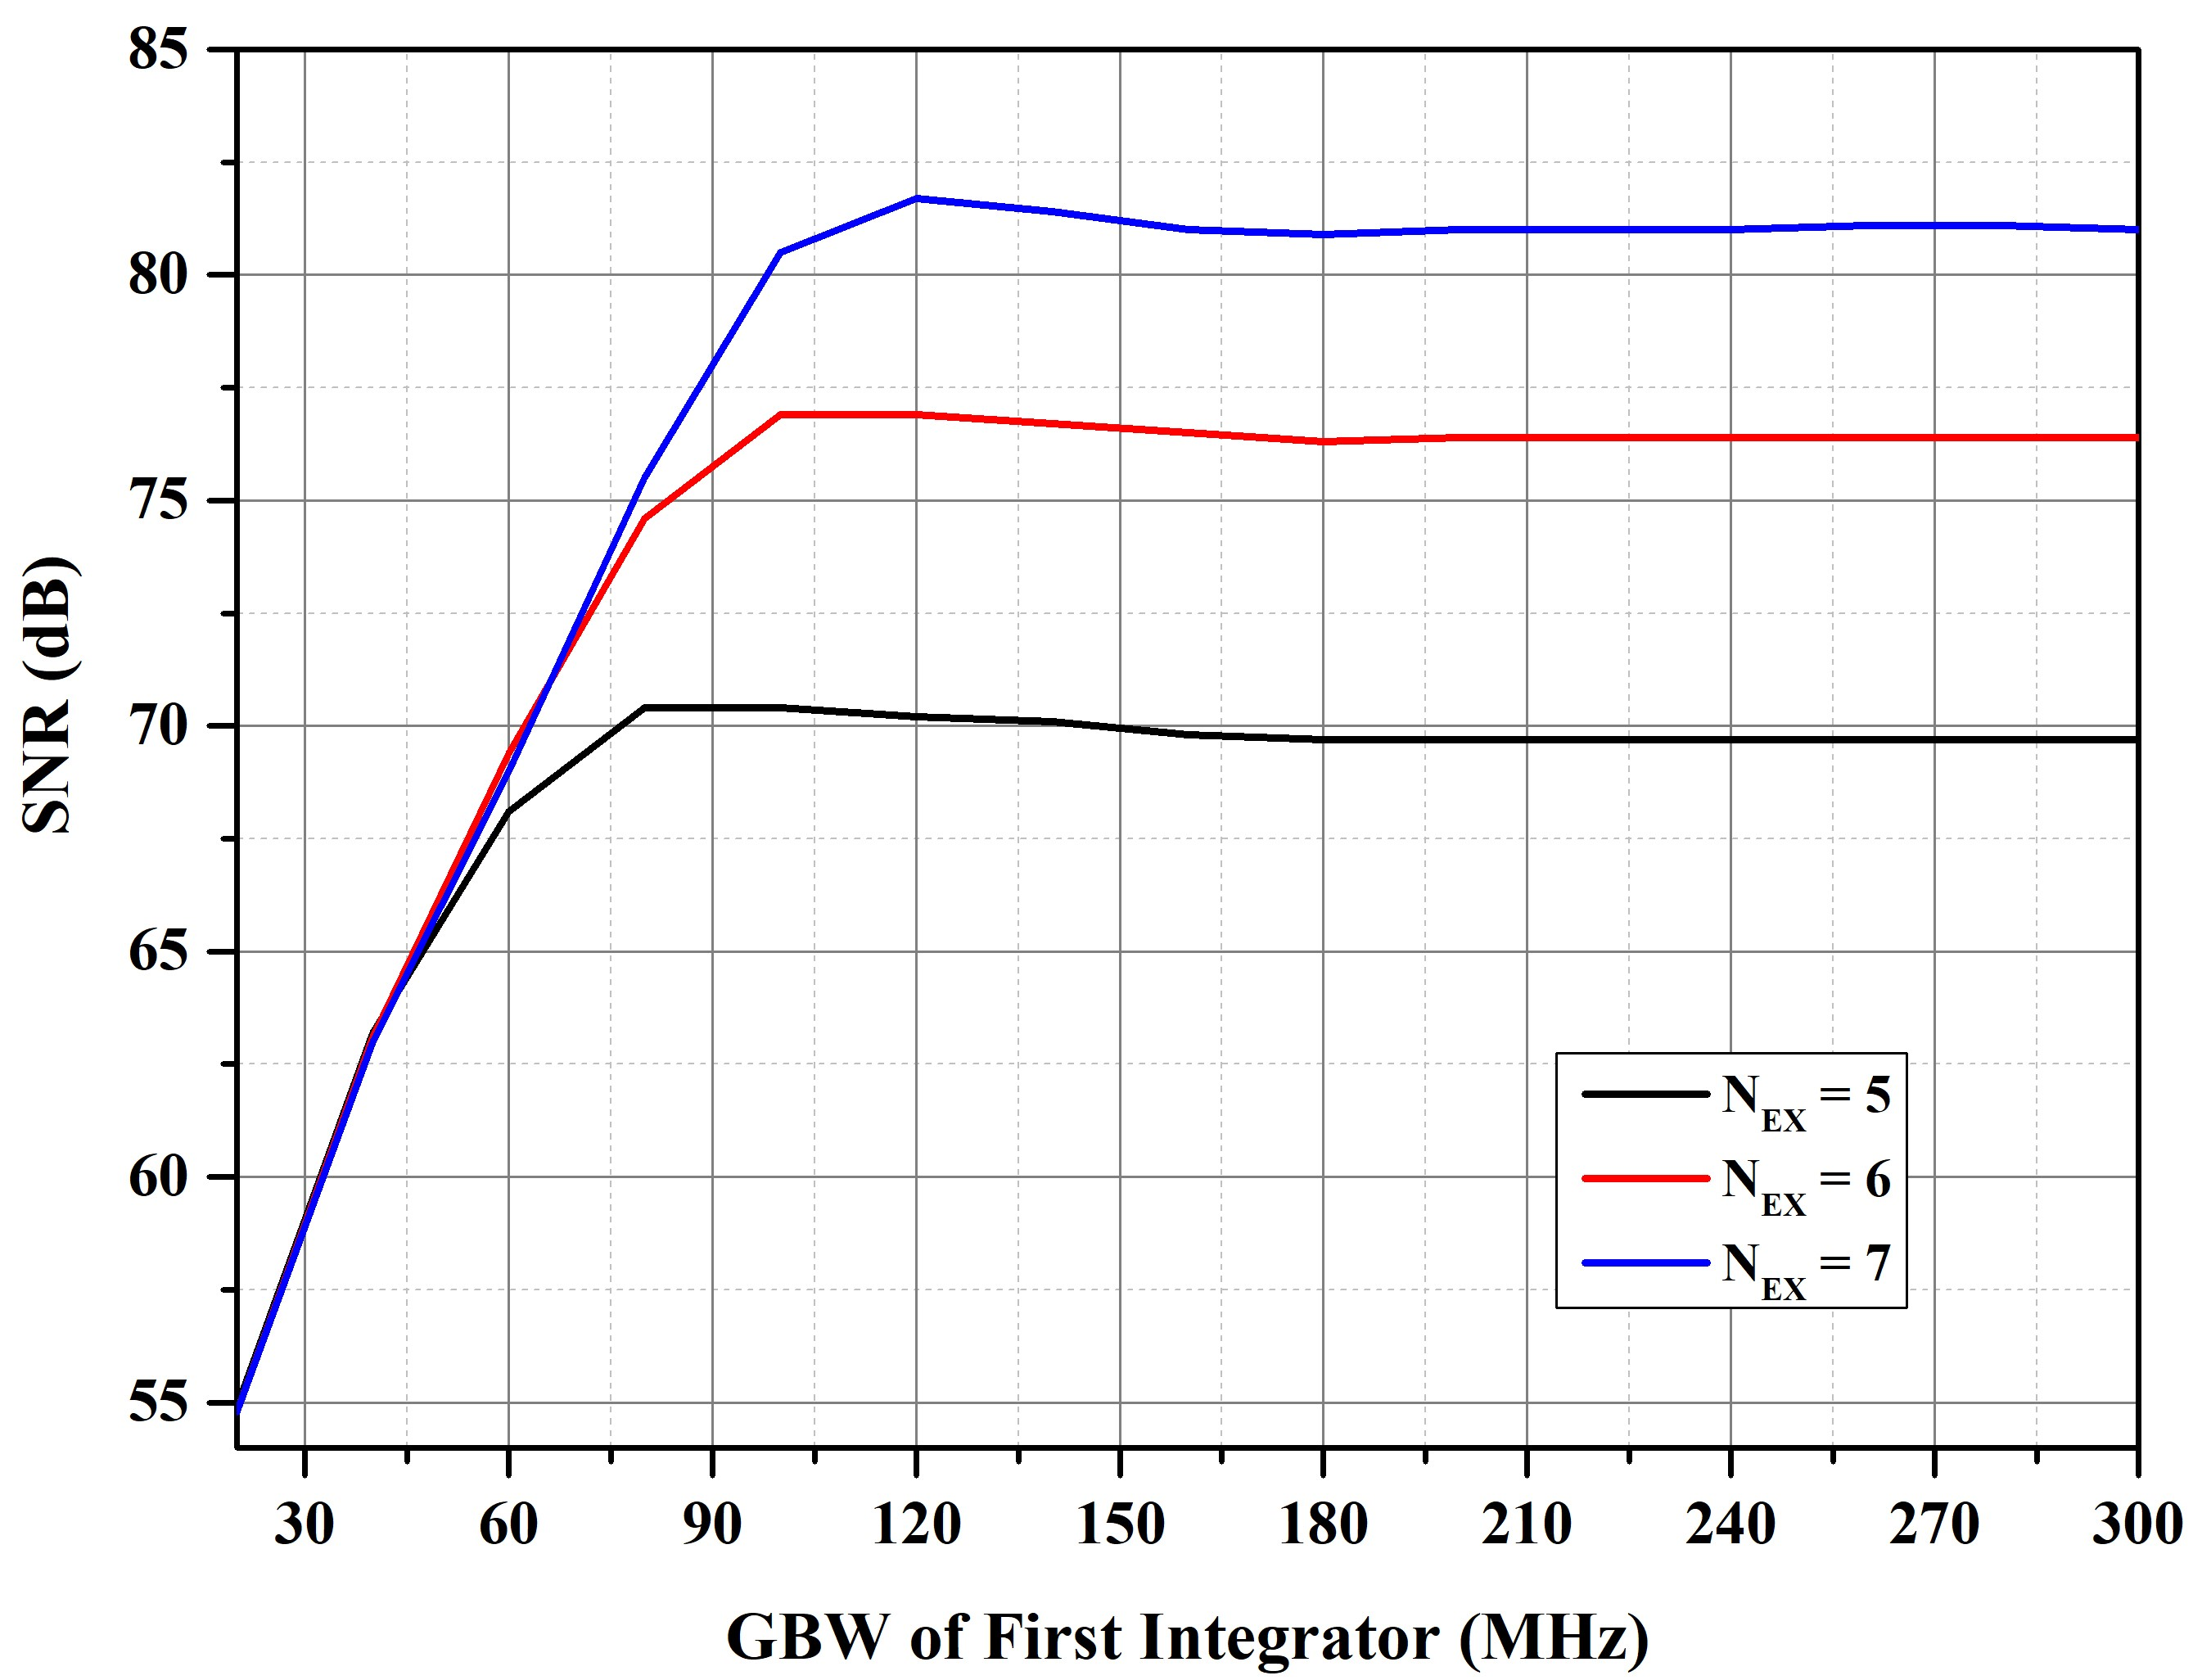
\includegraphics[scale=.28]{Chap04/Figures/snr_vs_gbw1_nsd2.jpg}
%     }
%     \qquad
%     \subfigure[]
%     {
%         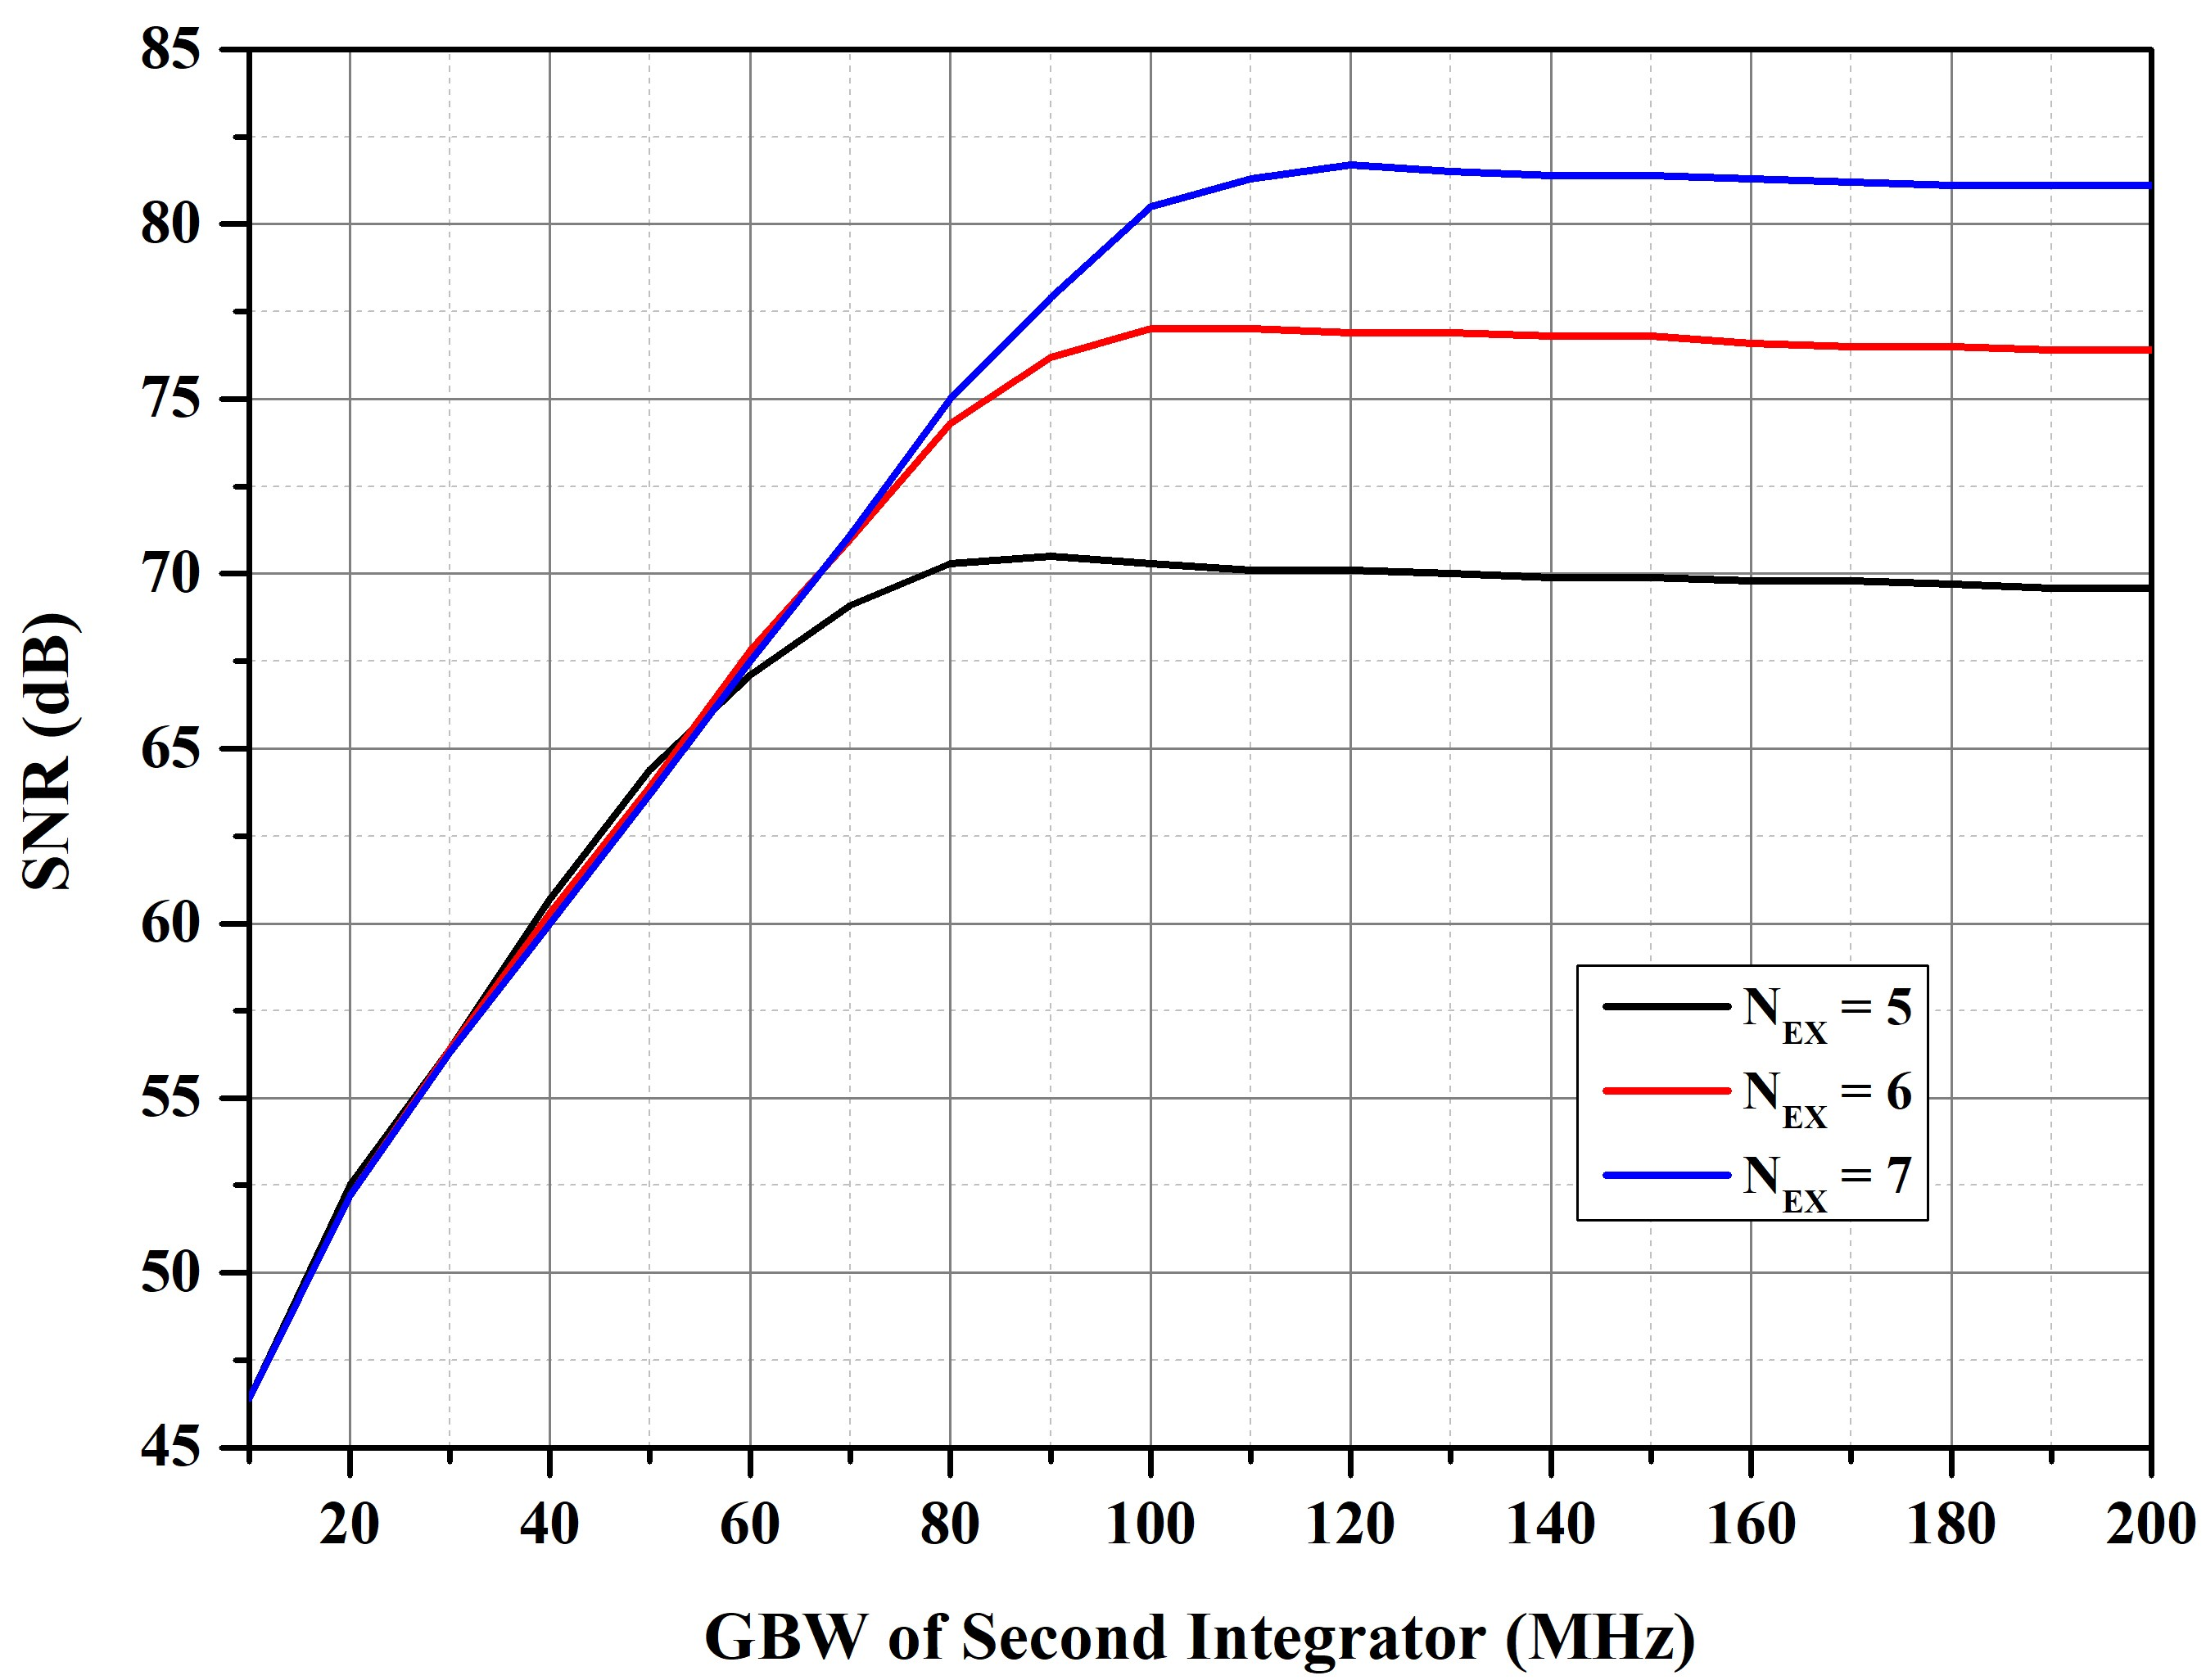
\includegraphics[scale=.28]{Chap04/Figures/snr_vs_gbw2_nsd2.jpg}
%     }
%     \caption
%     {
%         (a) GBW of the first Op-Amp Vs Overall SNR of the Extended Counting Incremental {\textSigma}{\textDelta} Modulator
%         (b) GBW of the second Op-Amp Vs Overall SNR of the Extended Counting Incremental {\textSigma}{\textDelta} Modulator
%     }
%     \label{GBW_Vs_SNR_NSD2}
% \end{figure}

% \begin{figure}[h]
%     \centering
%     \subfigure[]
%     {
%         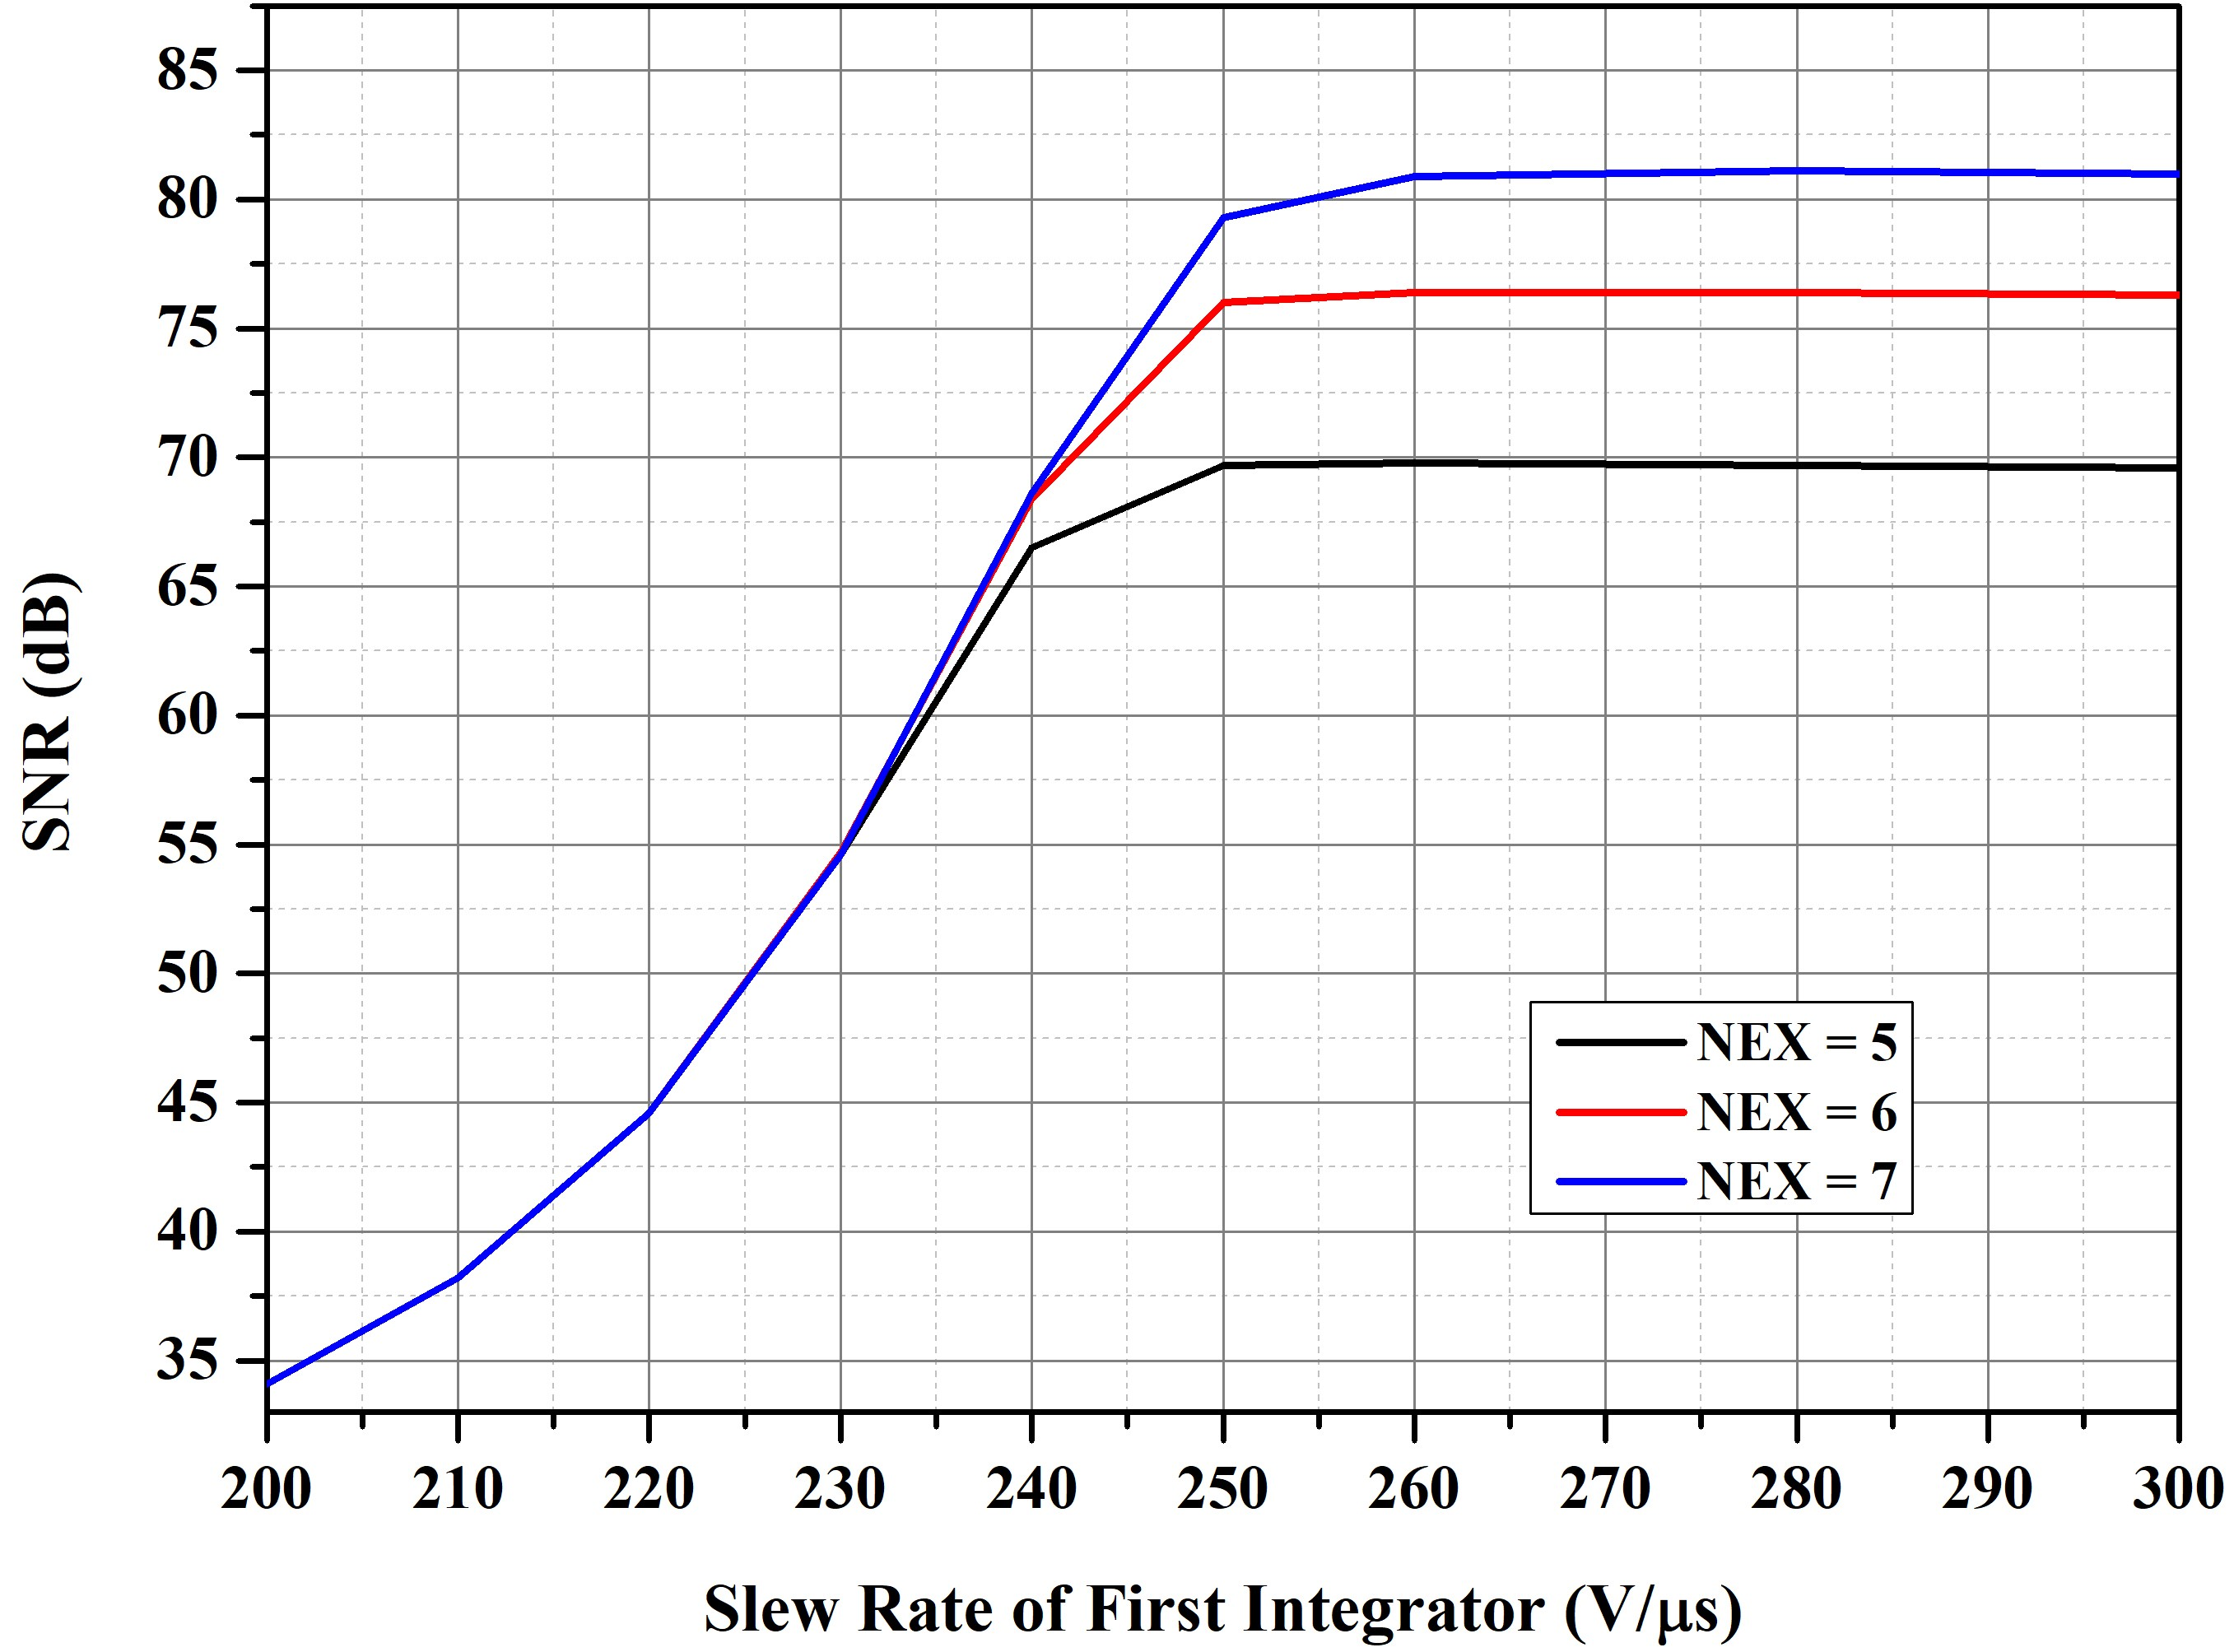
\includegraphics[scale=.28]{Chap04/Figures/snr_vs_sr1_nsd2.jpg}
%     }
%     \qquad
%     \subfigure[]
%     {
%         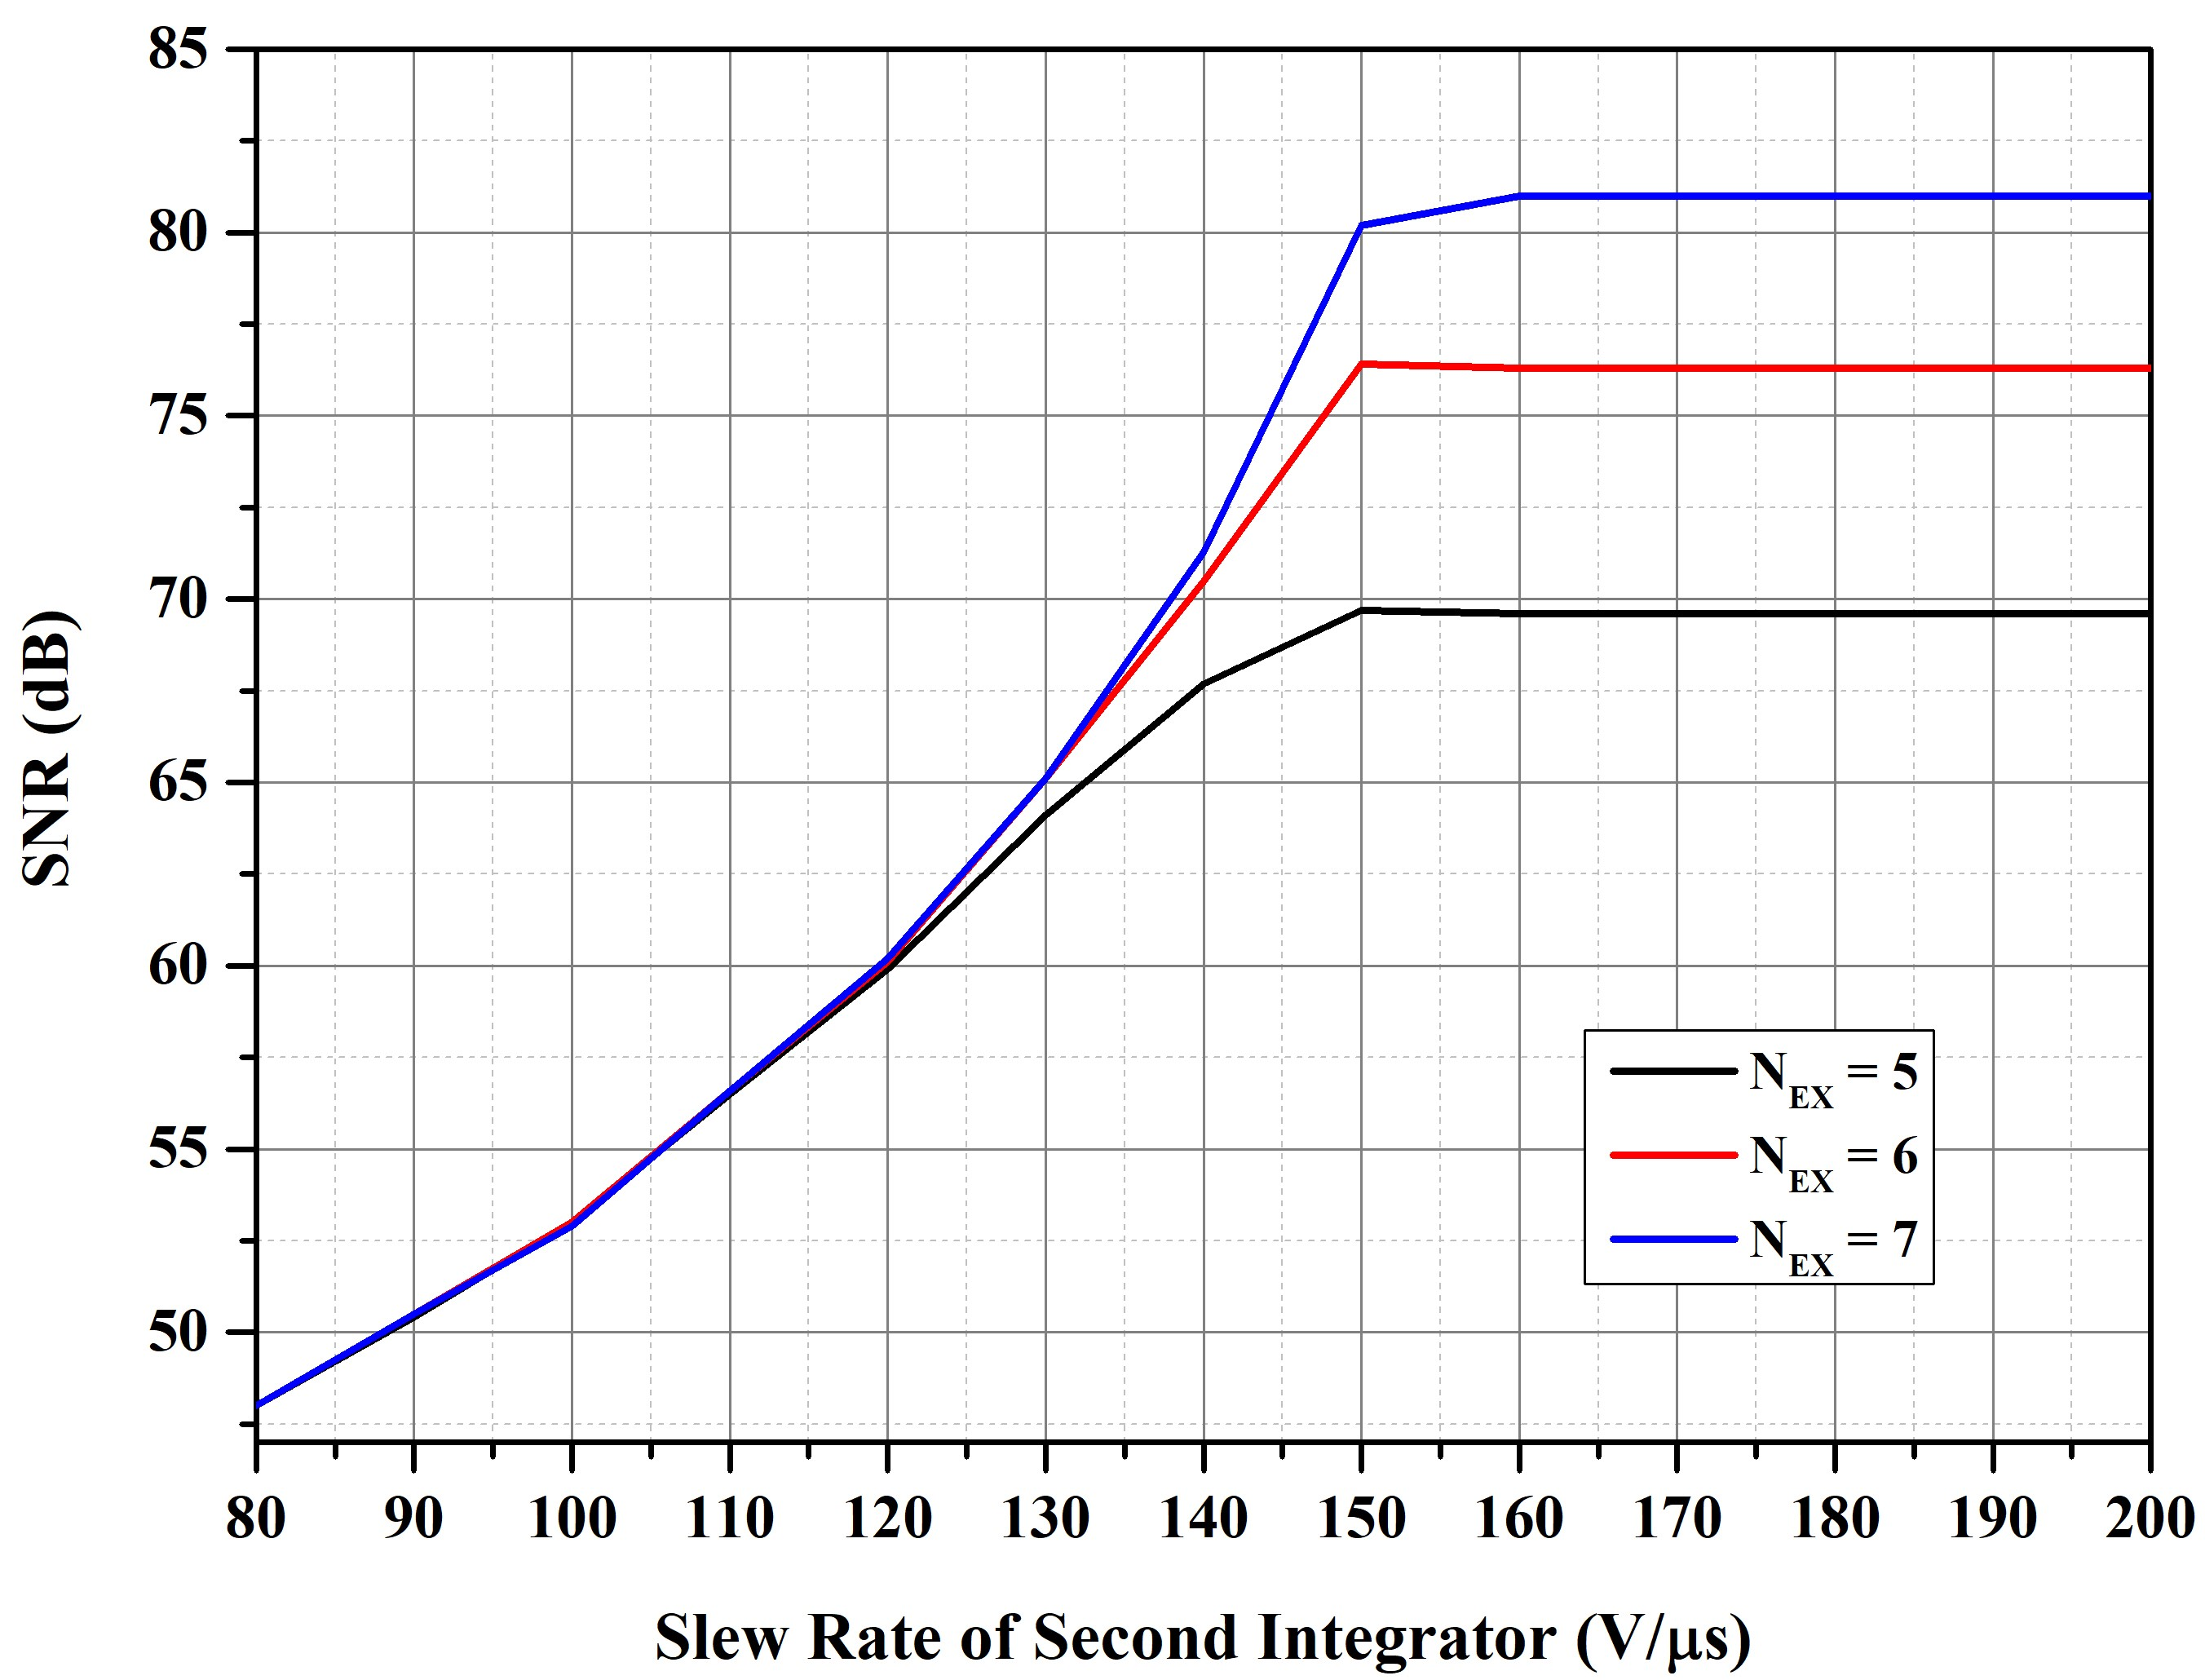
\includegraphics[scale=.28]{Chap04/Figures/snr_vs_sr2_nsd2.jpg}
%     }
%     \caption
%     {
%         (a) Slew Rate of the first Op-Amp Vs Overall SNR of the Extended Counting Incremental {\textSigma}{\textDelta} Modulator
%         (b) Slew Rate of the second Op-Amp Vs Overall SNR of the Extended Counting Incremental {\textSigma}{\textDelta} Modulator
%     }
%     \label{SR_Vs_SNR_NSD2}
% \end{figure}


% \begin{figure}[h]
%     \centering
%     \subfigure[]
%     {
%         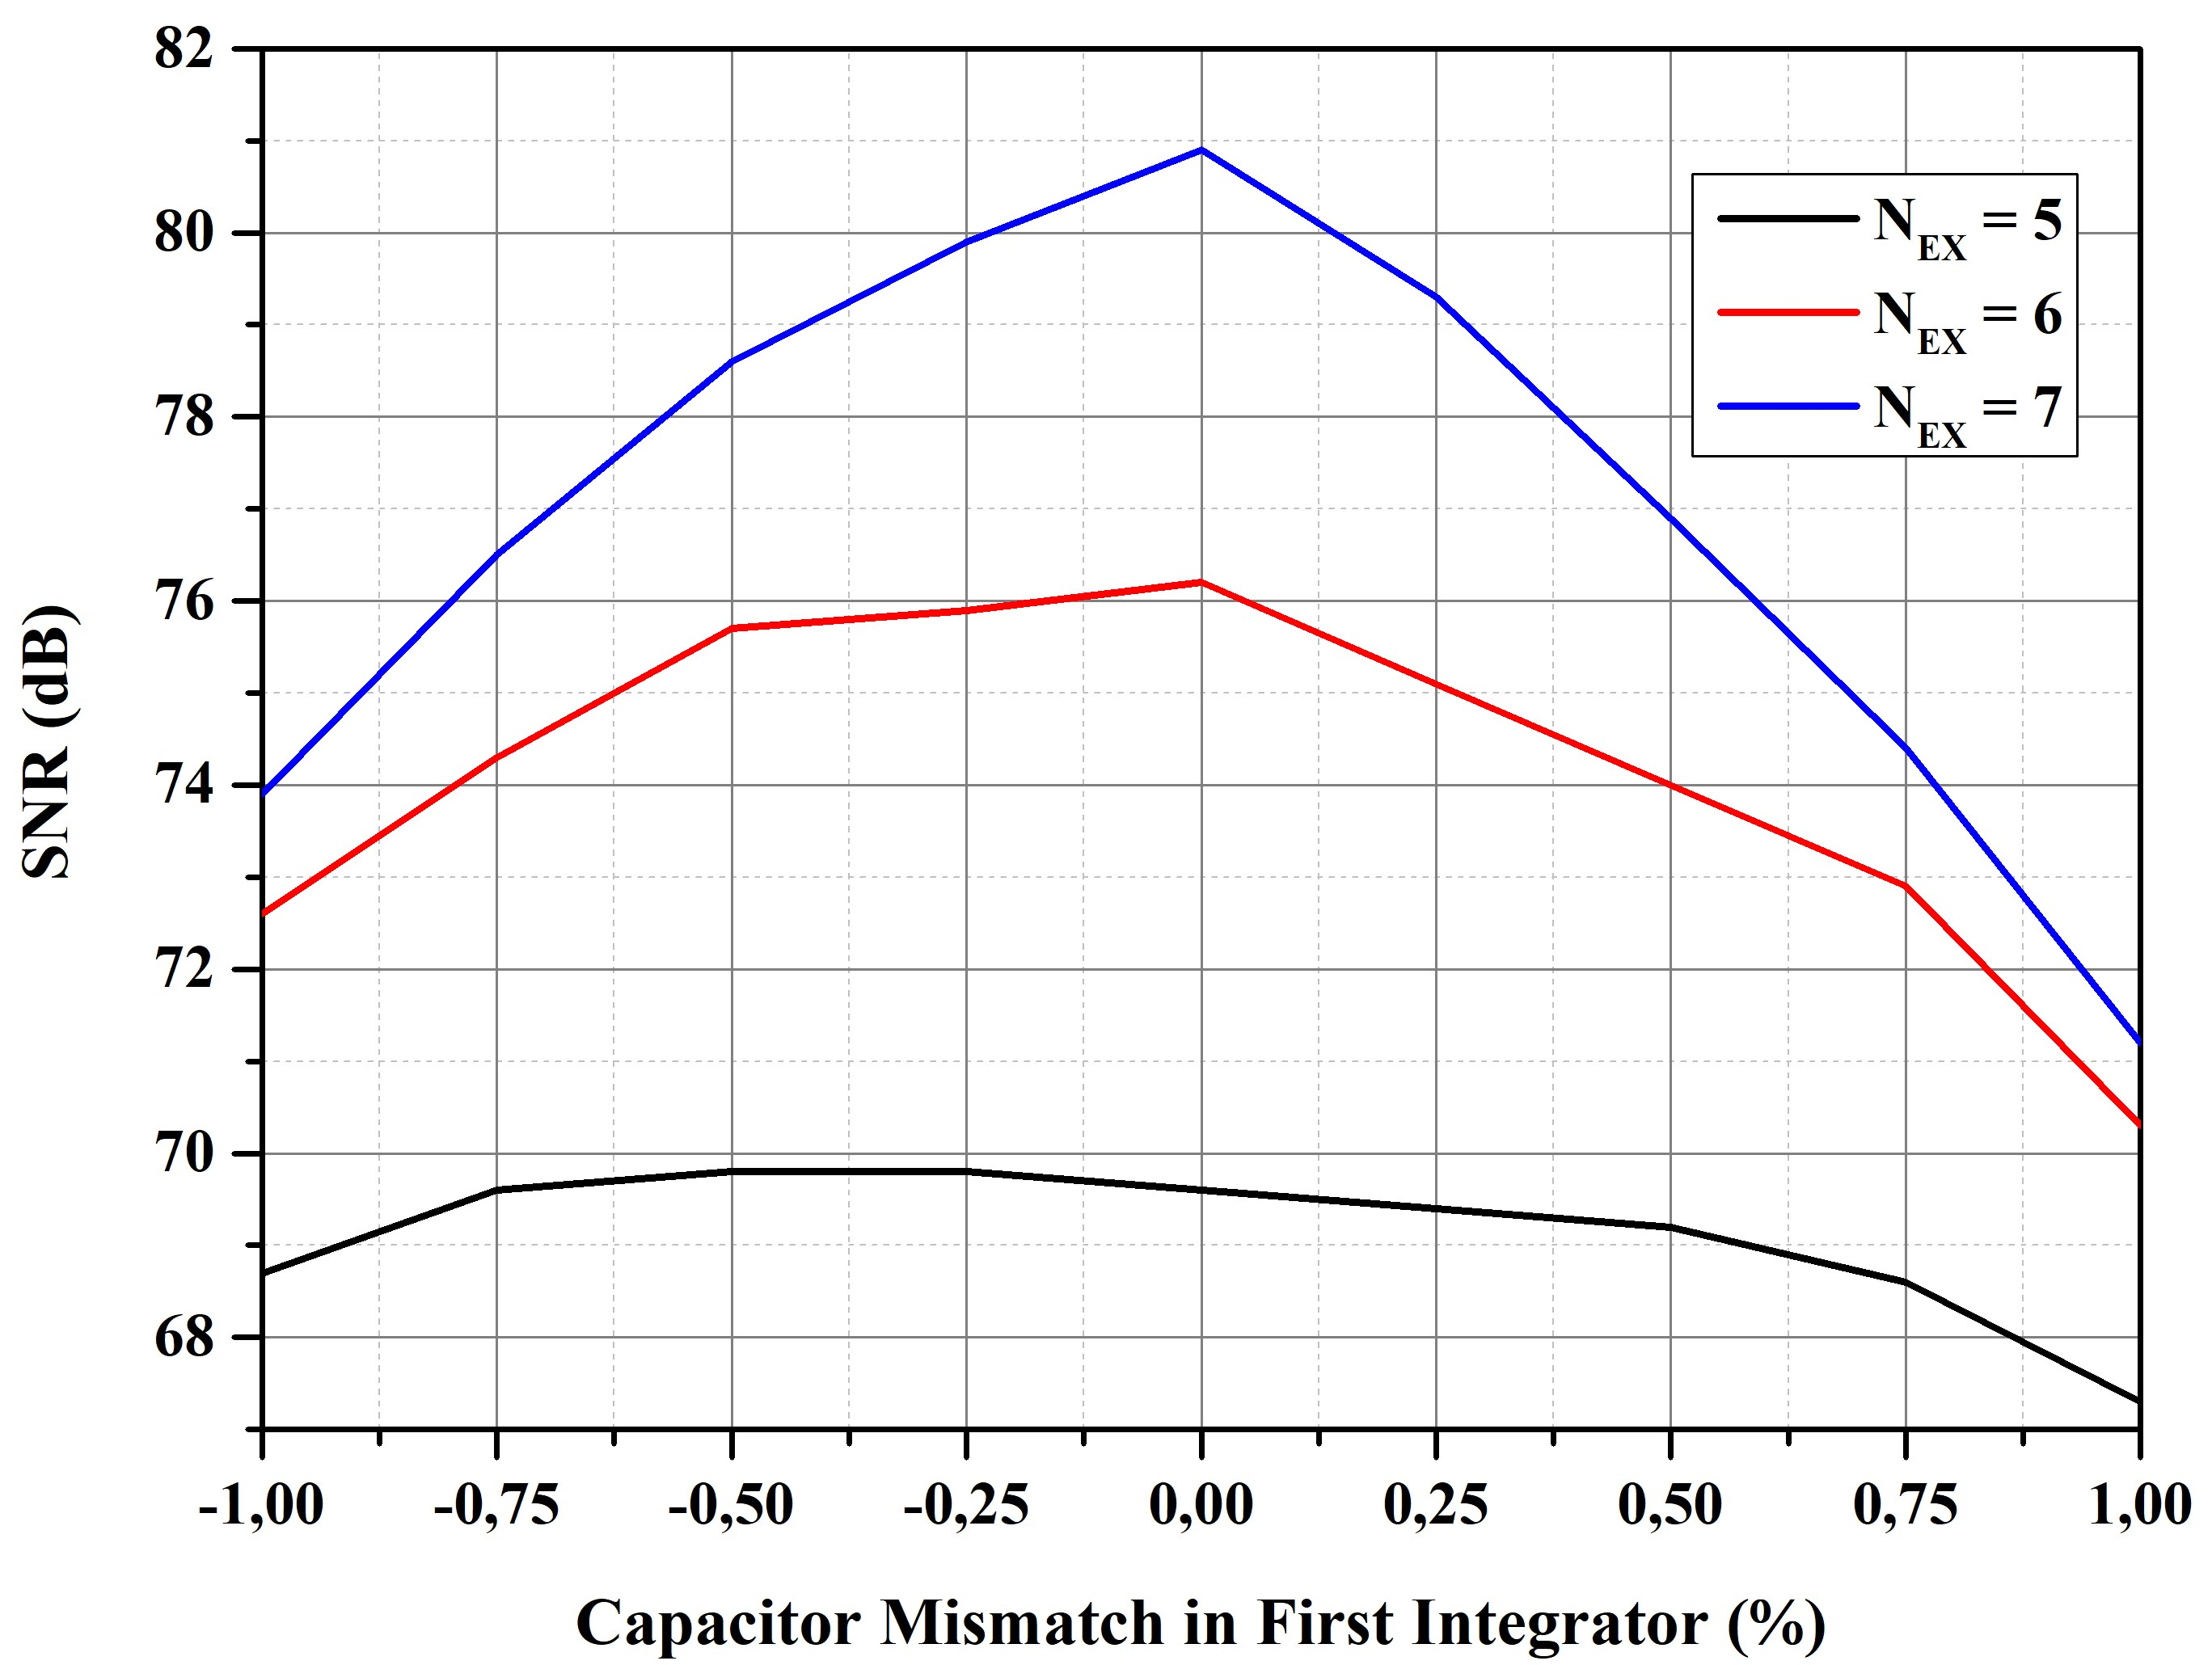
\includegraphics[scale=.28]{Chap04/Figures/snr_vs_capmis1_nsd2.jpg}
%     }
%     \qquad
%     \subfigure[]
%     {
%         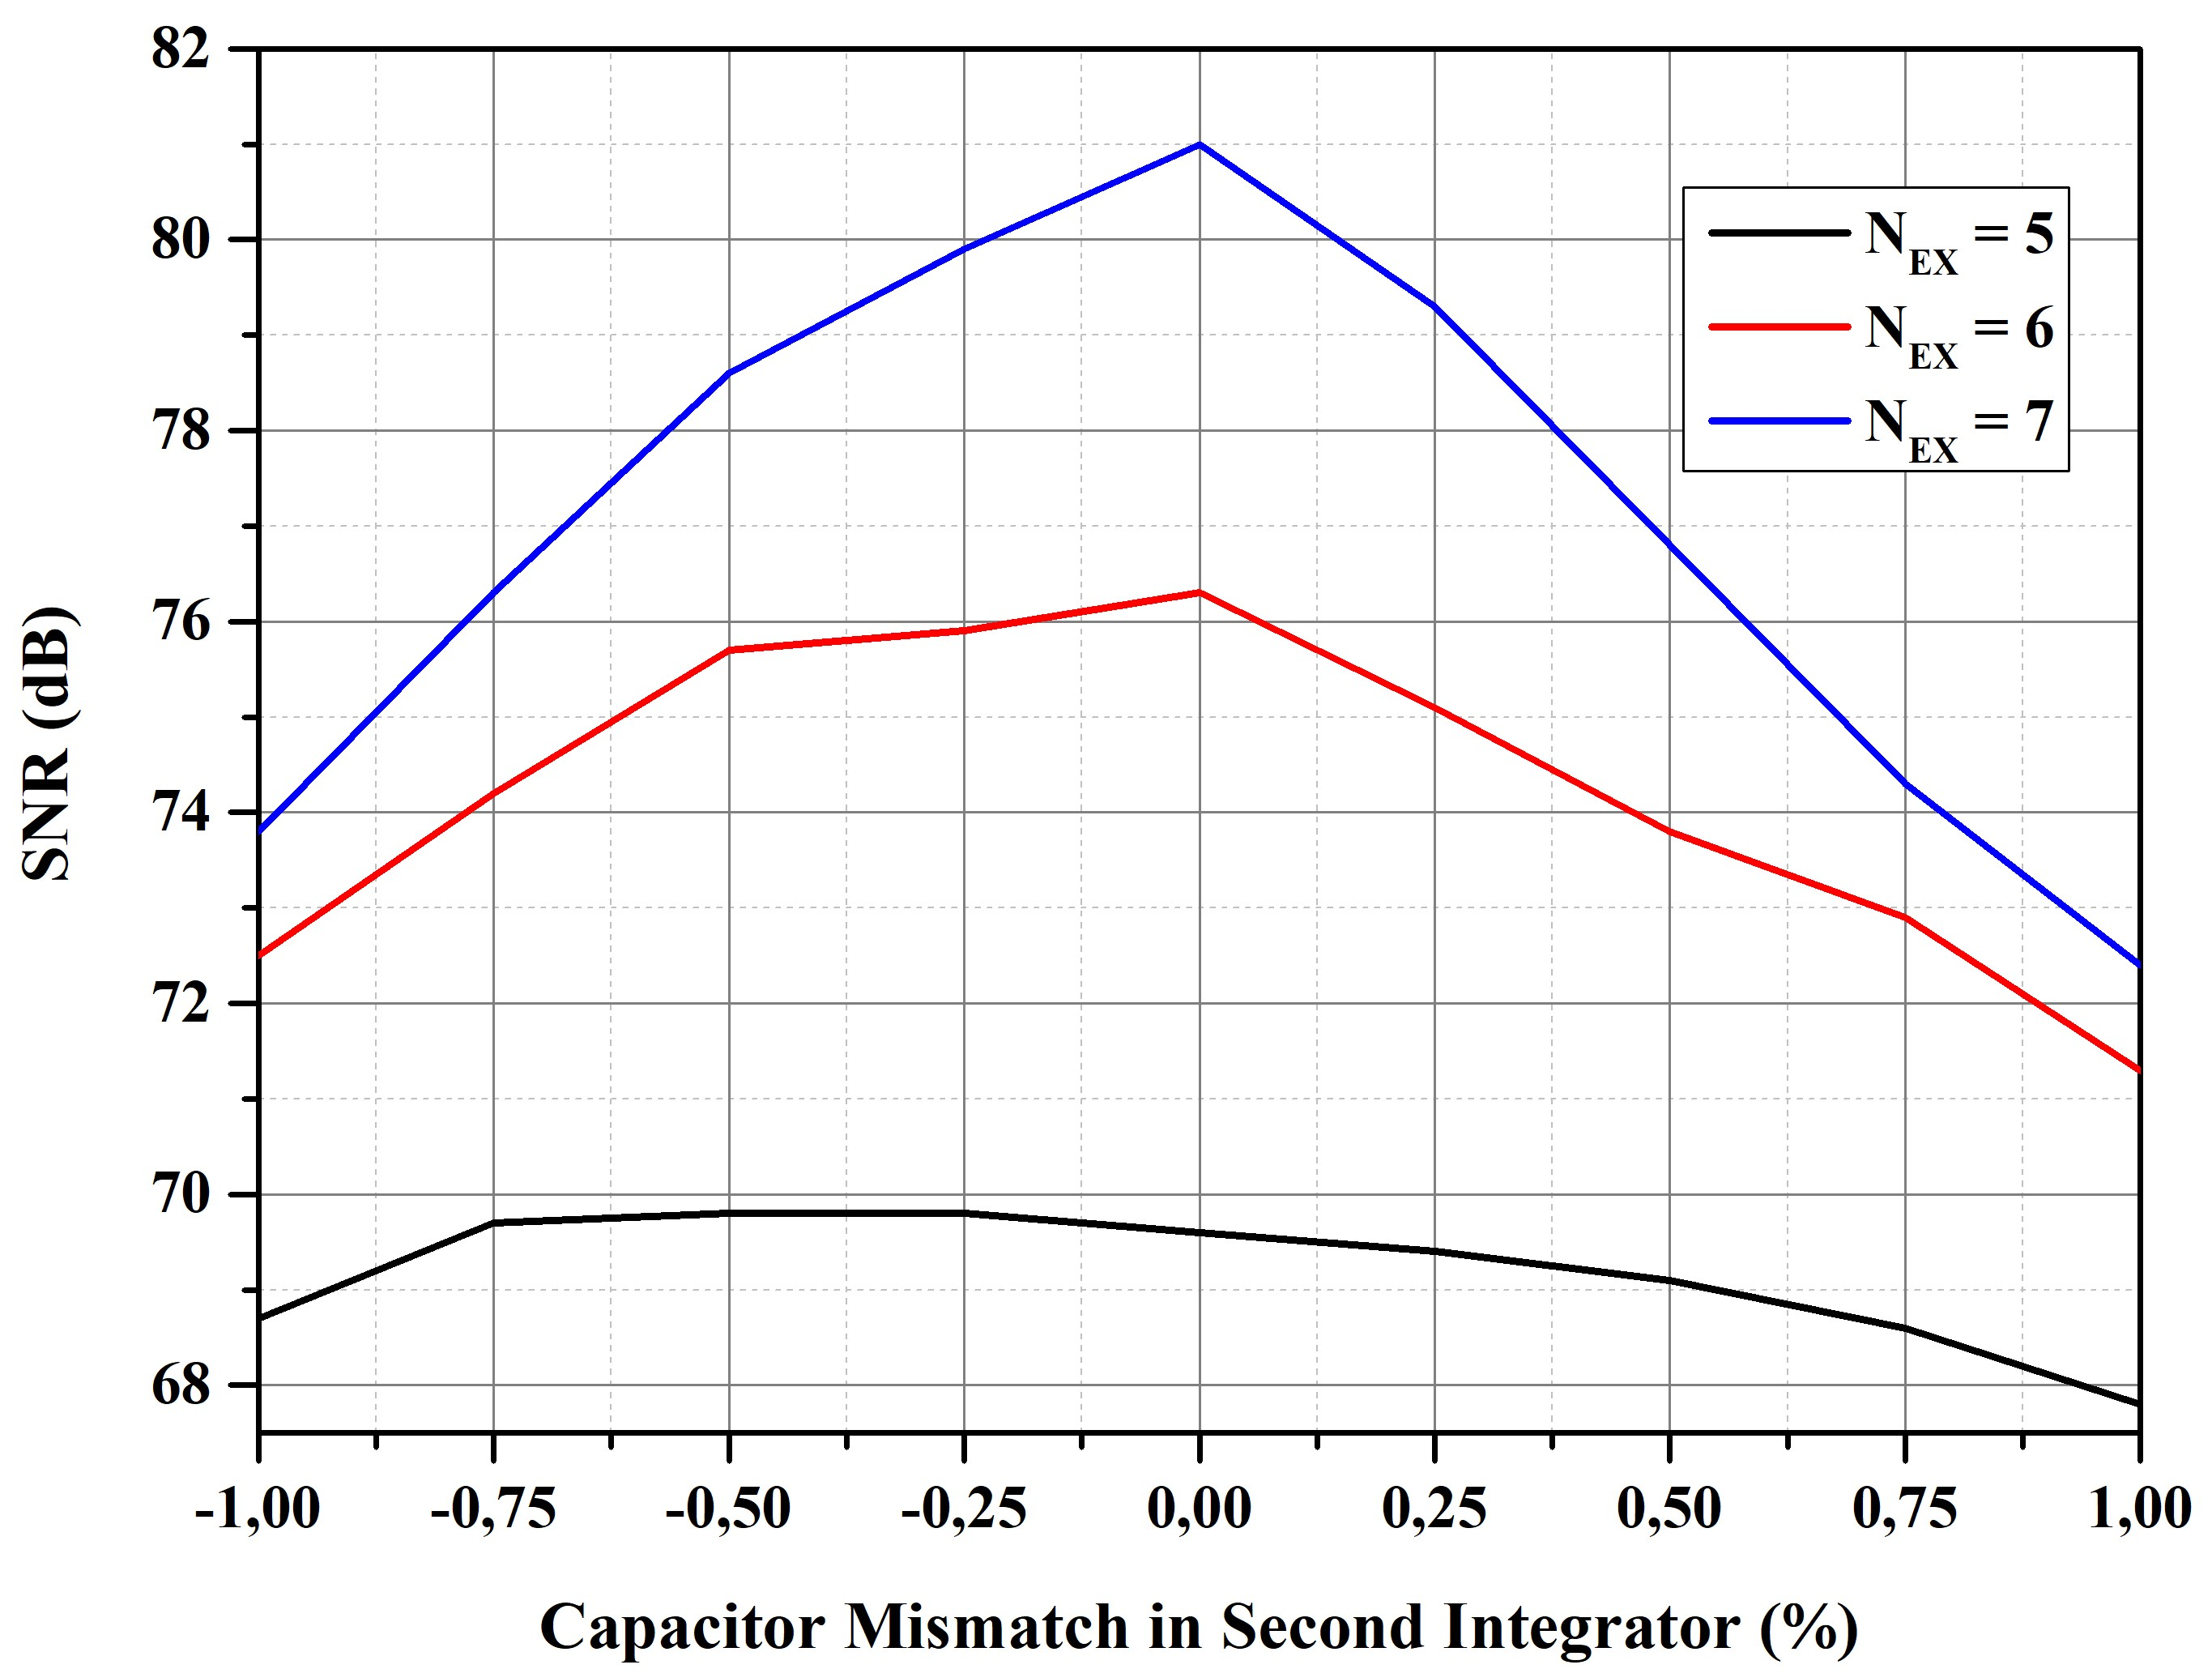
\includegraphics[scale=.28]{Chap04/Figures/snr_vs_capmis2_nsd2.jpg}
%     }
%     \caption
%     {
%         (a) Capacitor-mismatch of the first Op-Amp Vs Overall SNR of the Extended Counting Incremental {\textSigma}{\textDelta} Modulator
%         (b) Capacitor-mismatch of the second Op-Amp Vs Overall SNR of the Extended Counting Incremental {\textSigma}{\textDelta} Modulator
%     }
%     \label{CAPMIS_Vs_SNR_NSD2}
% \end{figure}

% \subsection{For I{\textSigma}{\textDelta}M Resolution of 3:}
% Similar study of the dependence of non-idealities of the op-amp and the capacitor ratio mismatch is been carried out over the architecture with I{\textSigma}{\textDelta}M quantizer resolution of 3-bit while resolution of the quantizer in the residual ADC is varied. Fig. \ref{SNR_GAIN_NSD3} shows the change in the overall SNR with respect to the low frequency gain. For having a maximum SNR, the least requirement of the gain of the op-amps is 60 dB. Similarly from Fig. \ref{GBW_Vs_SNR_NSD3} it can be inferred that necessary GBWs of the first op-amp and the second op-amp for Extended rage ISDM to exhibit adequate SNDR are $200\ MHz$ and $140\ MHz$ respectively. Considering the SR of the op-amps, SR of $230\ V/\mu s$ for first op-amp and that of $120\ V/\mu s$ for the second op-amp is mandatory which is distinct from the Fig. \ref{SR_Vs_SNR_NSD3}. For the purpose of the capacitor mismatch study, it is obligatory to carry out the study in presence of the non-idealities of the op-amp, all the block specifications extracted from the tests carried out above (gain, GBW and SR) were substituted. Fig. \ref{CAPMIS_Vs_SNR_NSD3} shows the variation of the SNDR with respect to the percentage of capacitor mismatch in the first integrator and second integrator respectively. Comparing these architectures with one with $N_{SD} = 2$ (Fig. \ref{CAPMIS_Vs_SNR_NSD2}), the percentage of the drop in SNDR is lesser. 
% \begin{figure}[h]
% \centering
% 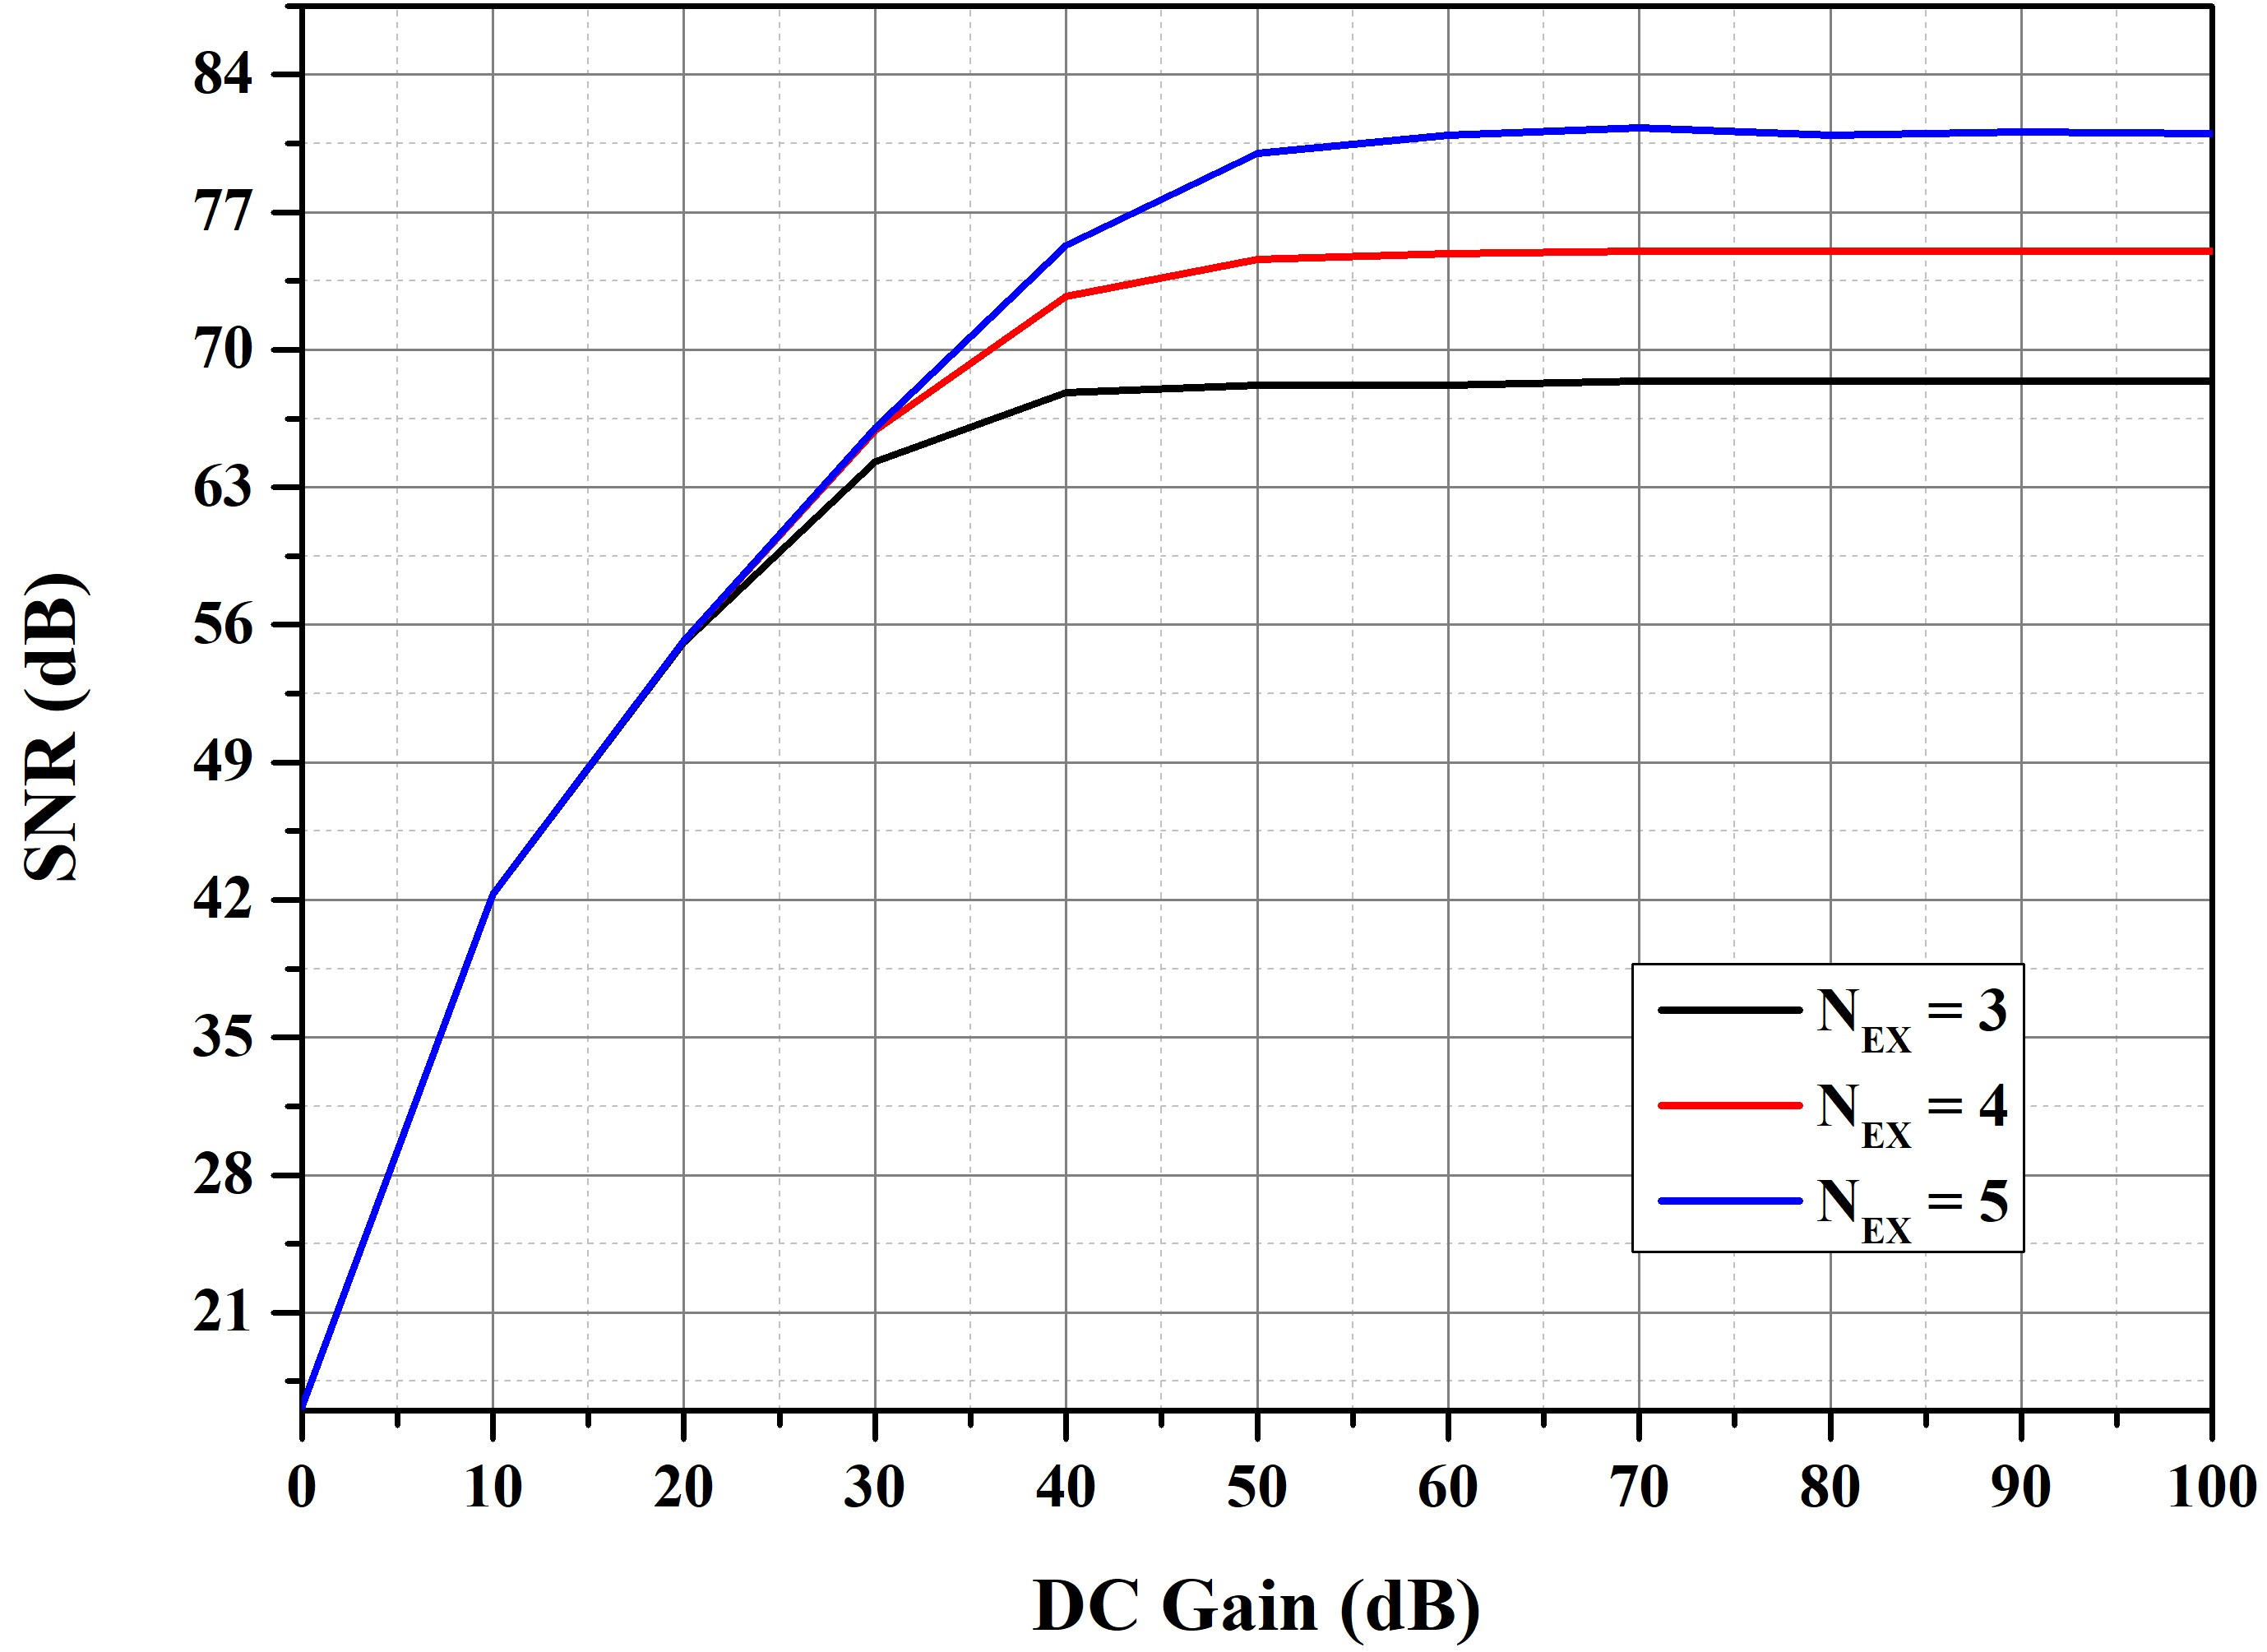
\includegraphics[width=0.5\columnwidth]{Chap04/Figures/snr_vs_gain_nsd3.jpg}
% \caption{Gain of the Op-Amps Vs Overall SNR of the Extended Counting Incremental {\textSigma}{\textDelta} Modulator}
% \label{SNR_GAIN_NSD3}
% \end{figure}
% \begin{figure}[h]
%     \centering
%     \subfigure[]
%     {
%         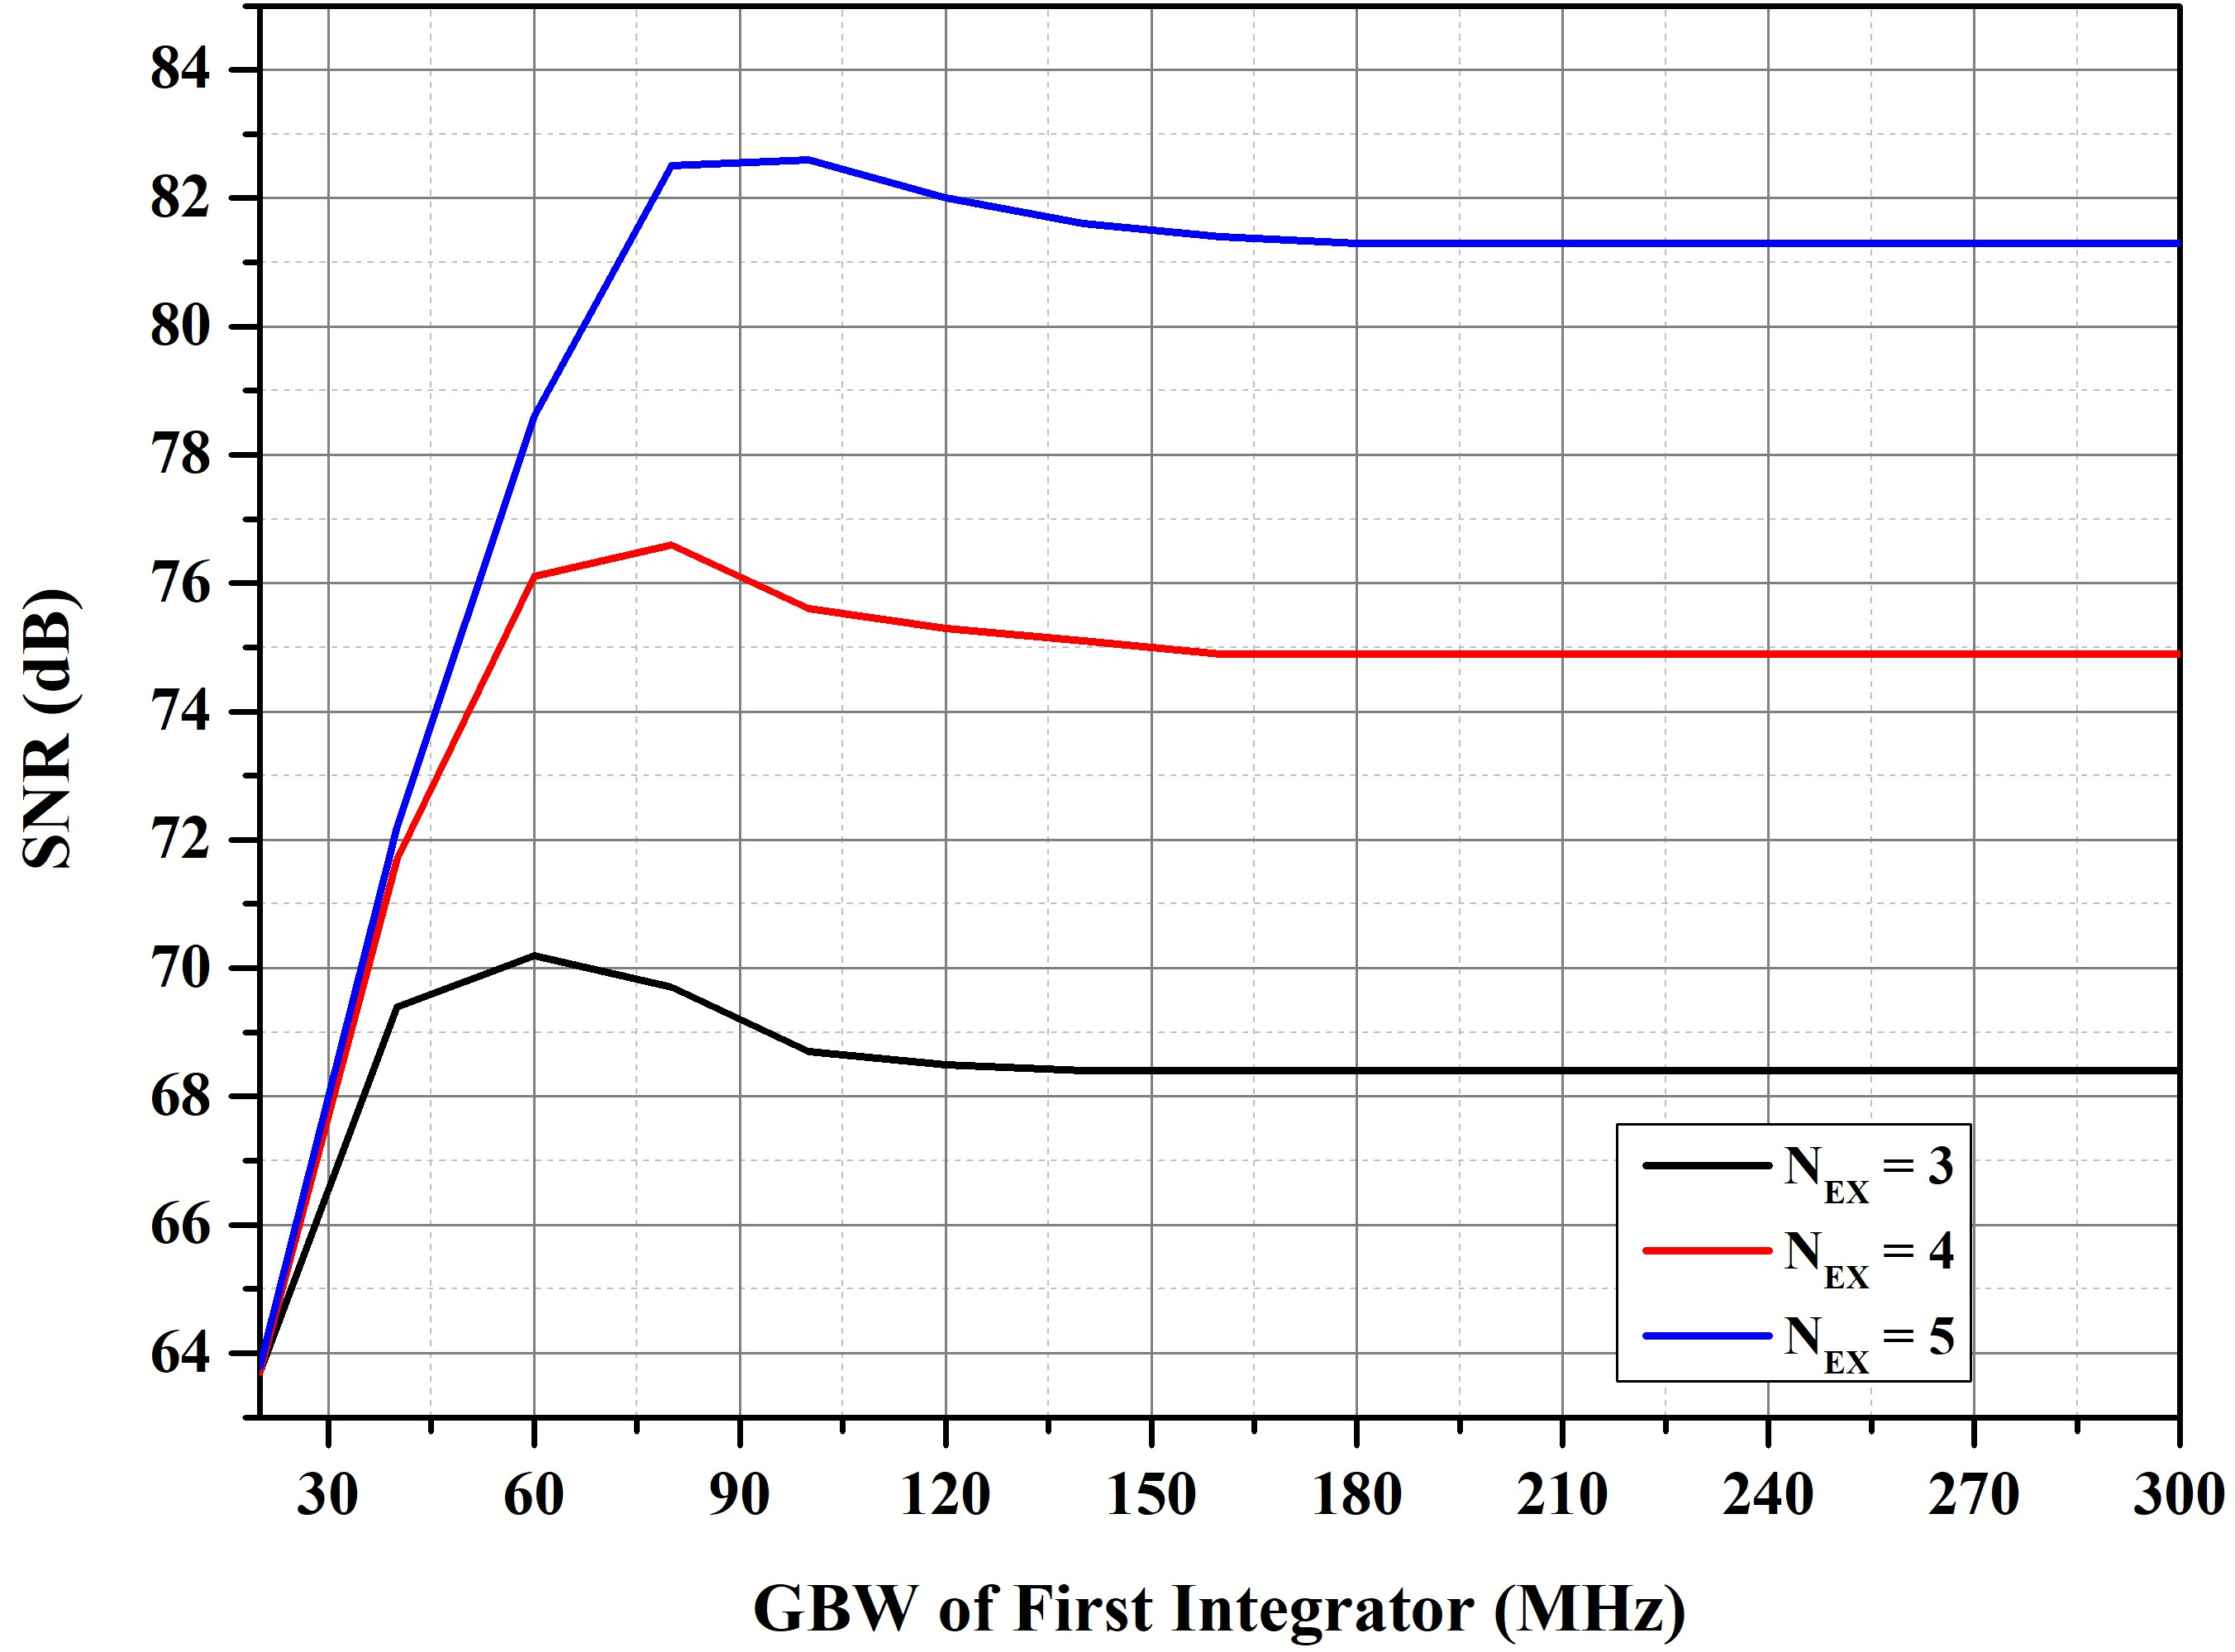
\includegraphics[scale=.28]{Chap04/Figures/snr_vs_gbw1_nsd3.jpg}
%     }
%     \qquad
%     \subfigure[]
%     {
%         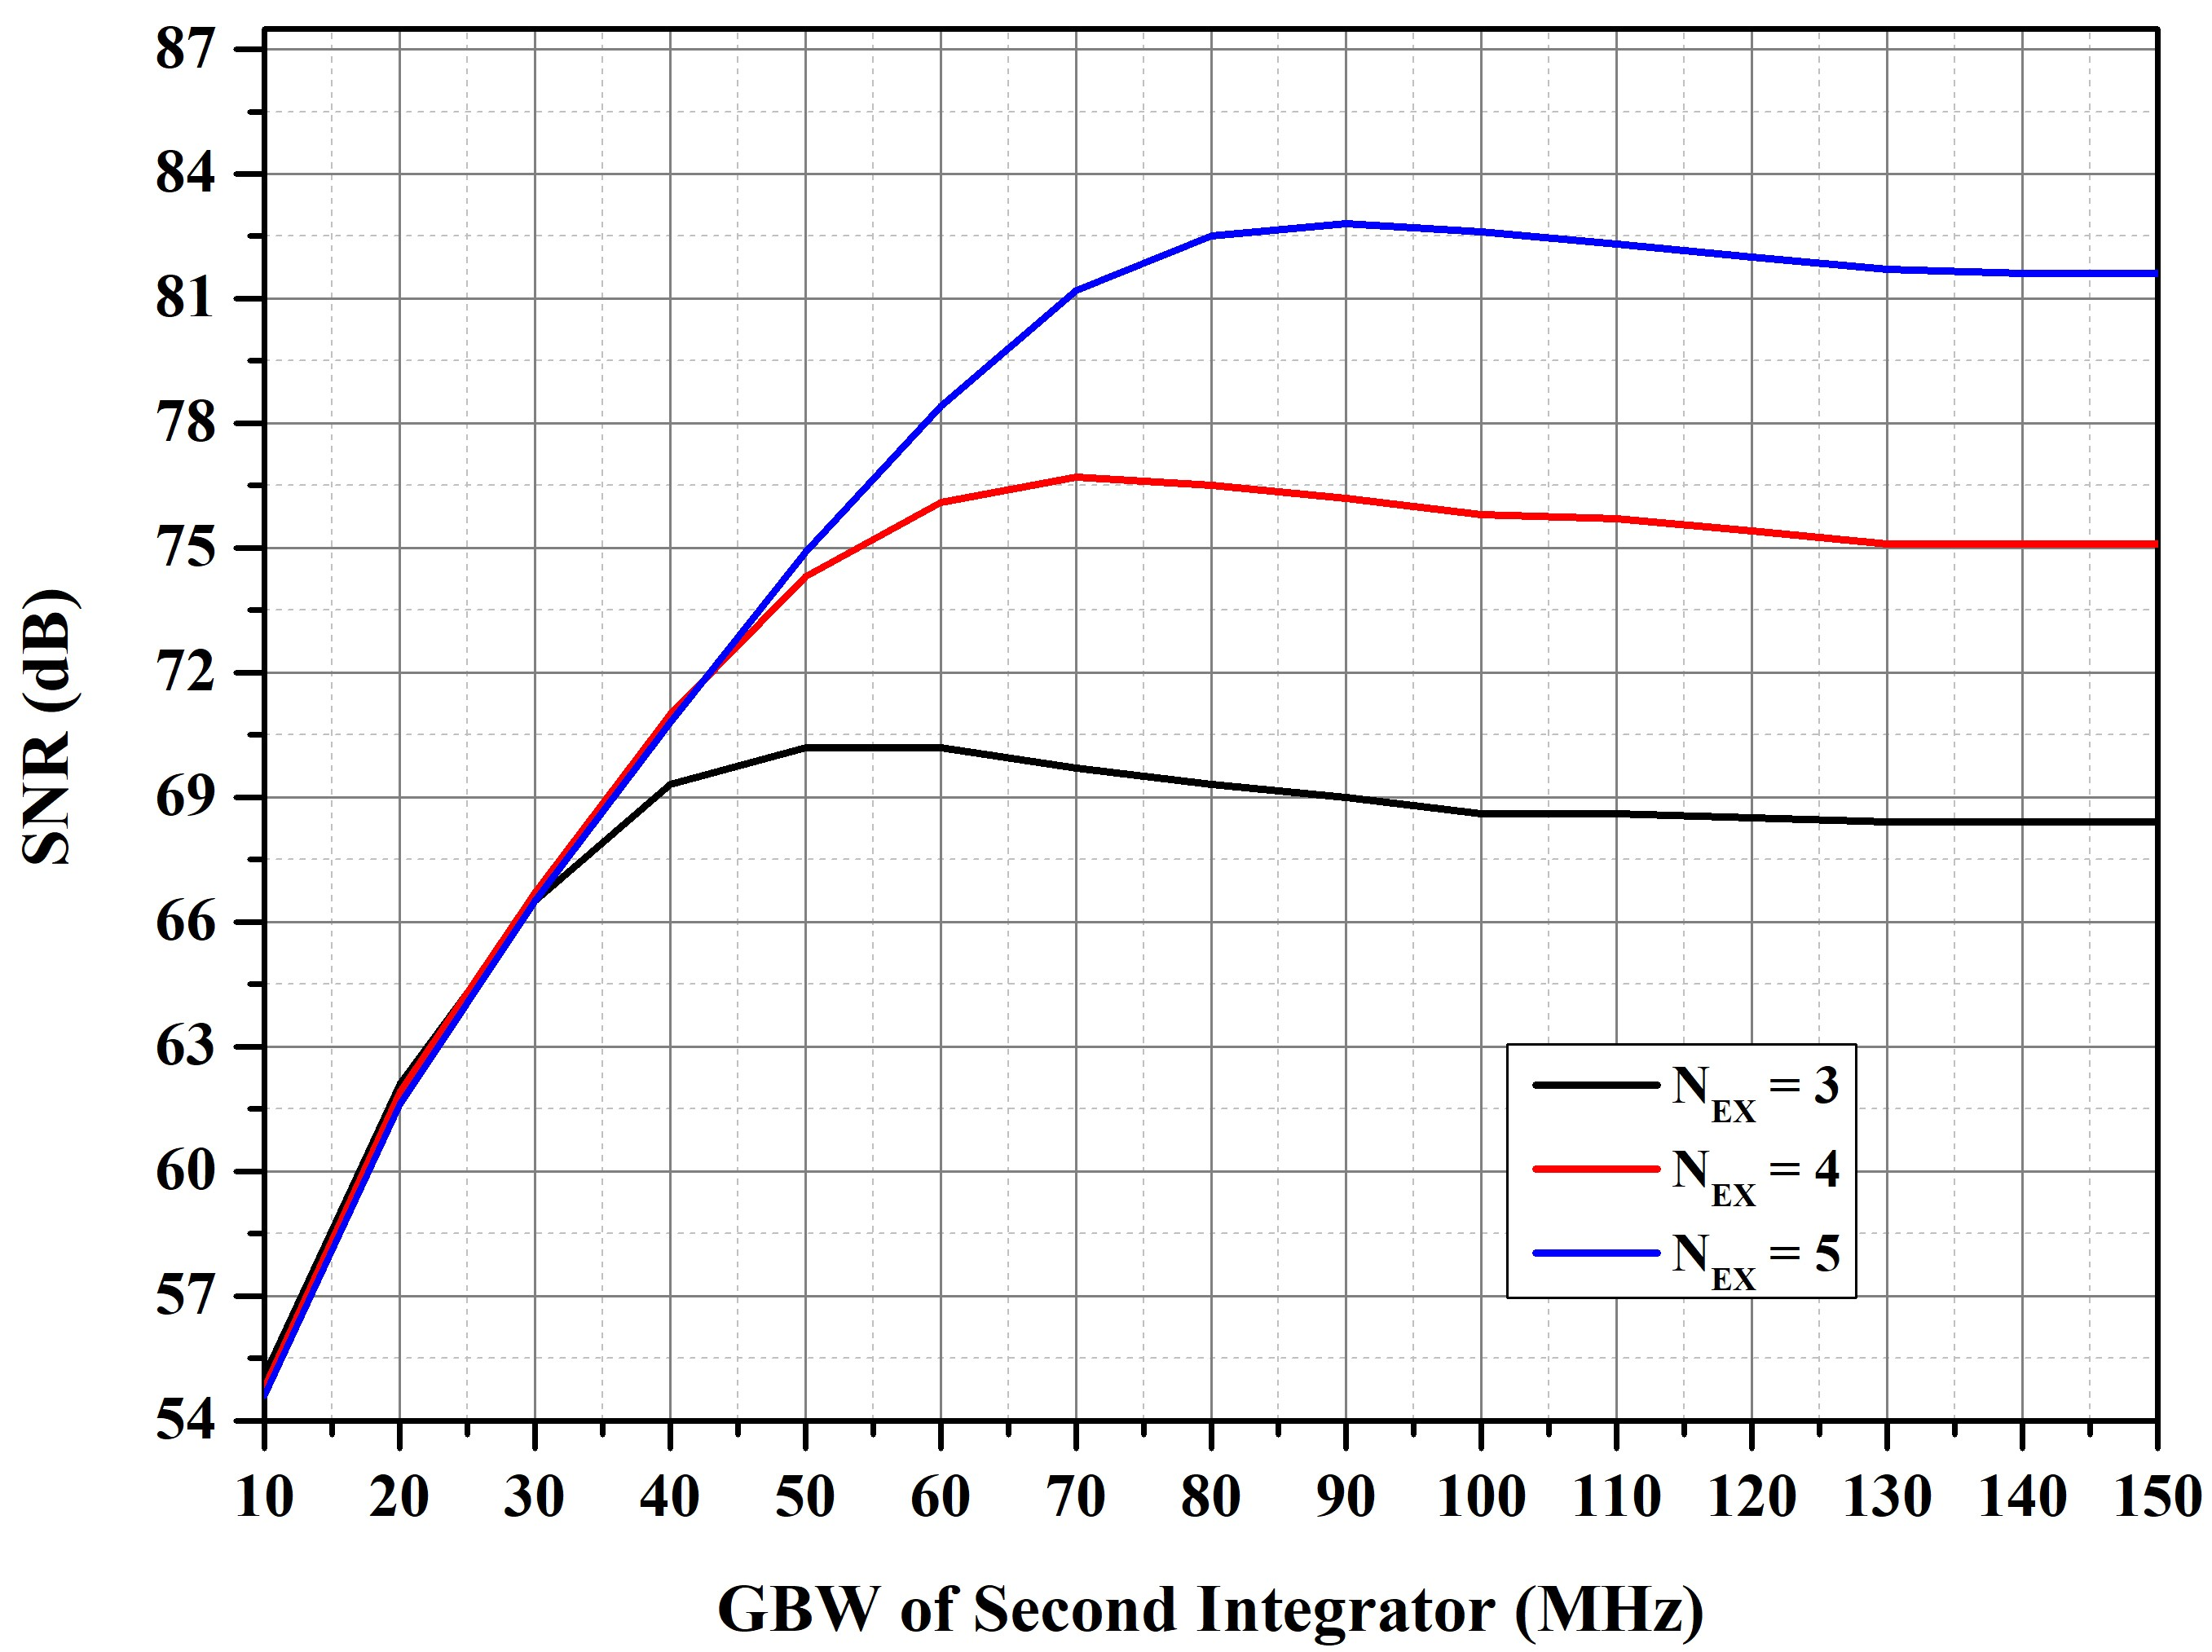
\includegraphics[scale=.28]{Chap04/Figures/snr_vs_gbw2_nsd3.jpg}
%     }
%     \caption
%     {
%         (a) GBW of the first Op-Amp Vs Overall SNR of the Extended Counting Incremental {\textSigma}{\textDelta} Modulator
%         (b) GBW of the second Op-Amp Vs Overall SNR of the Extended Counting Incremental {\textSigma}{\textDelta} Modulator
%     }
%     \label{GBW_Vs_SNR_NSD3}
% \end{figure}

% \begin{figure}[h]
%     \centering
%     \subfigure[]
%     {
%         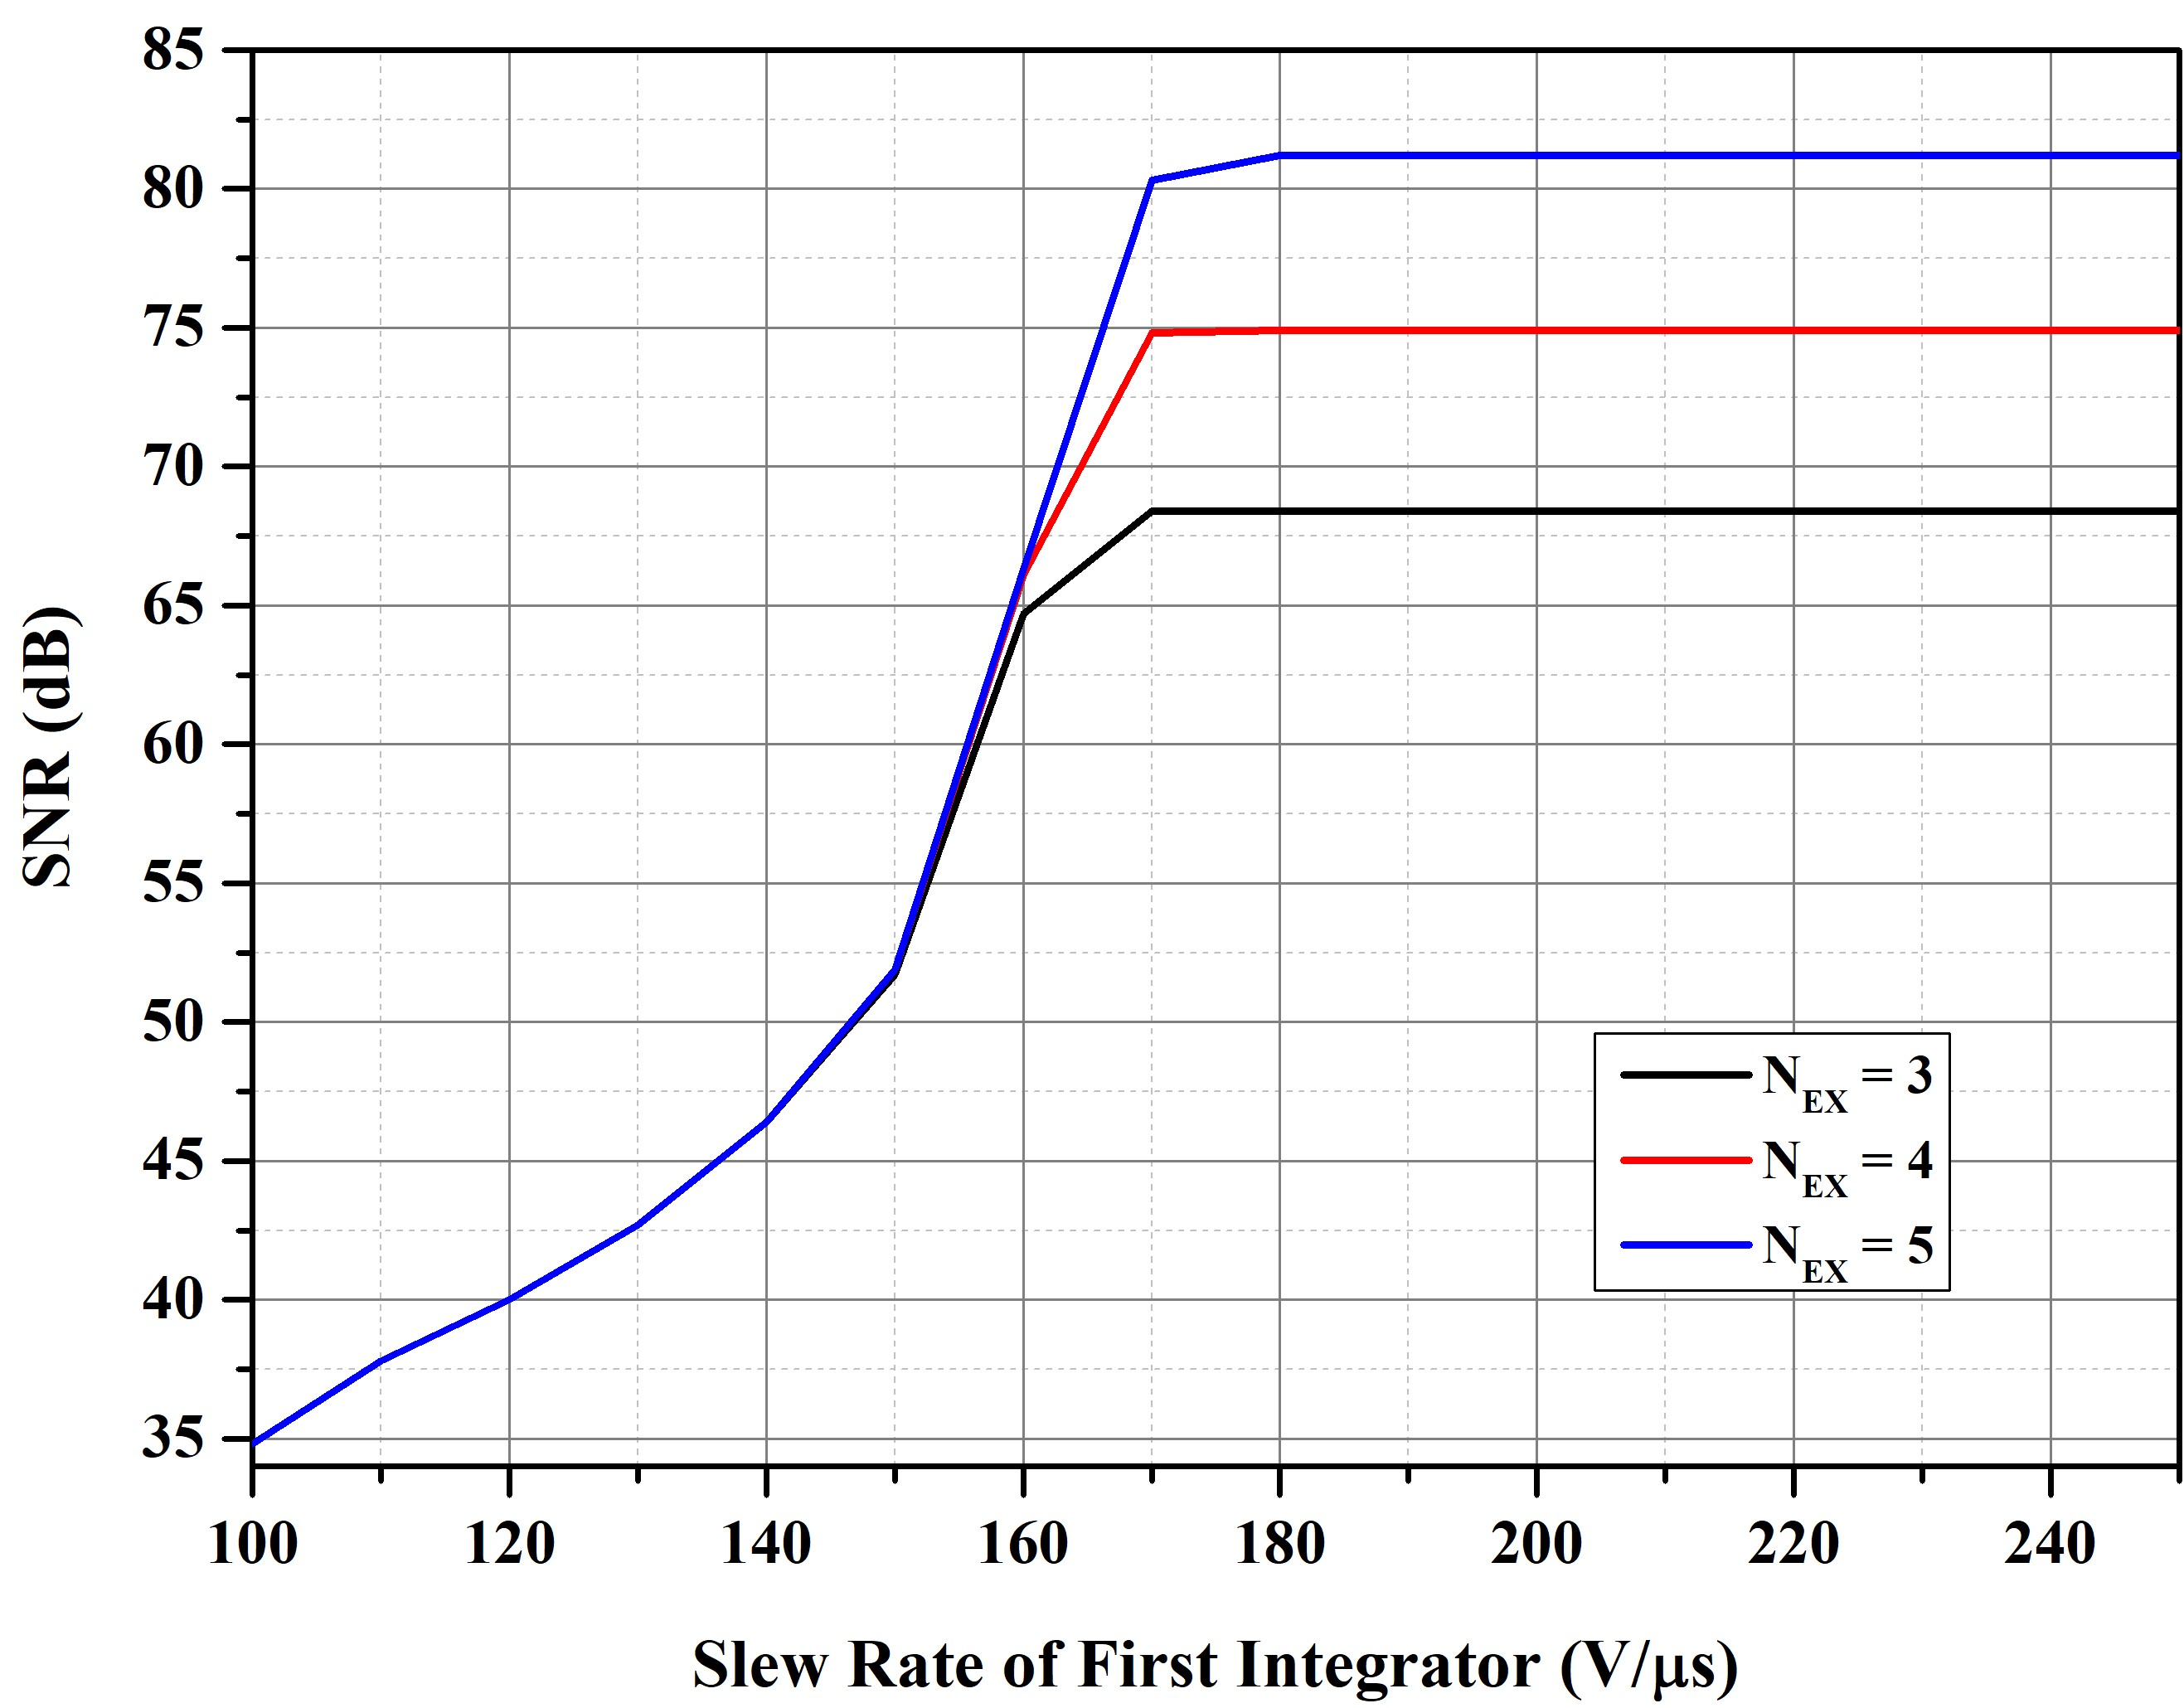
\includegraphics[scale=.28]{Chap04/Figures/snr_vs_sr1_nsd3.jpg}
%     }
%     \qquad
%     \subfigure[]
%     {
%         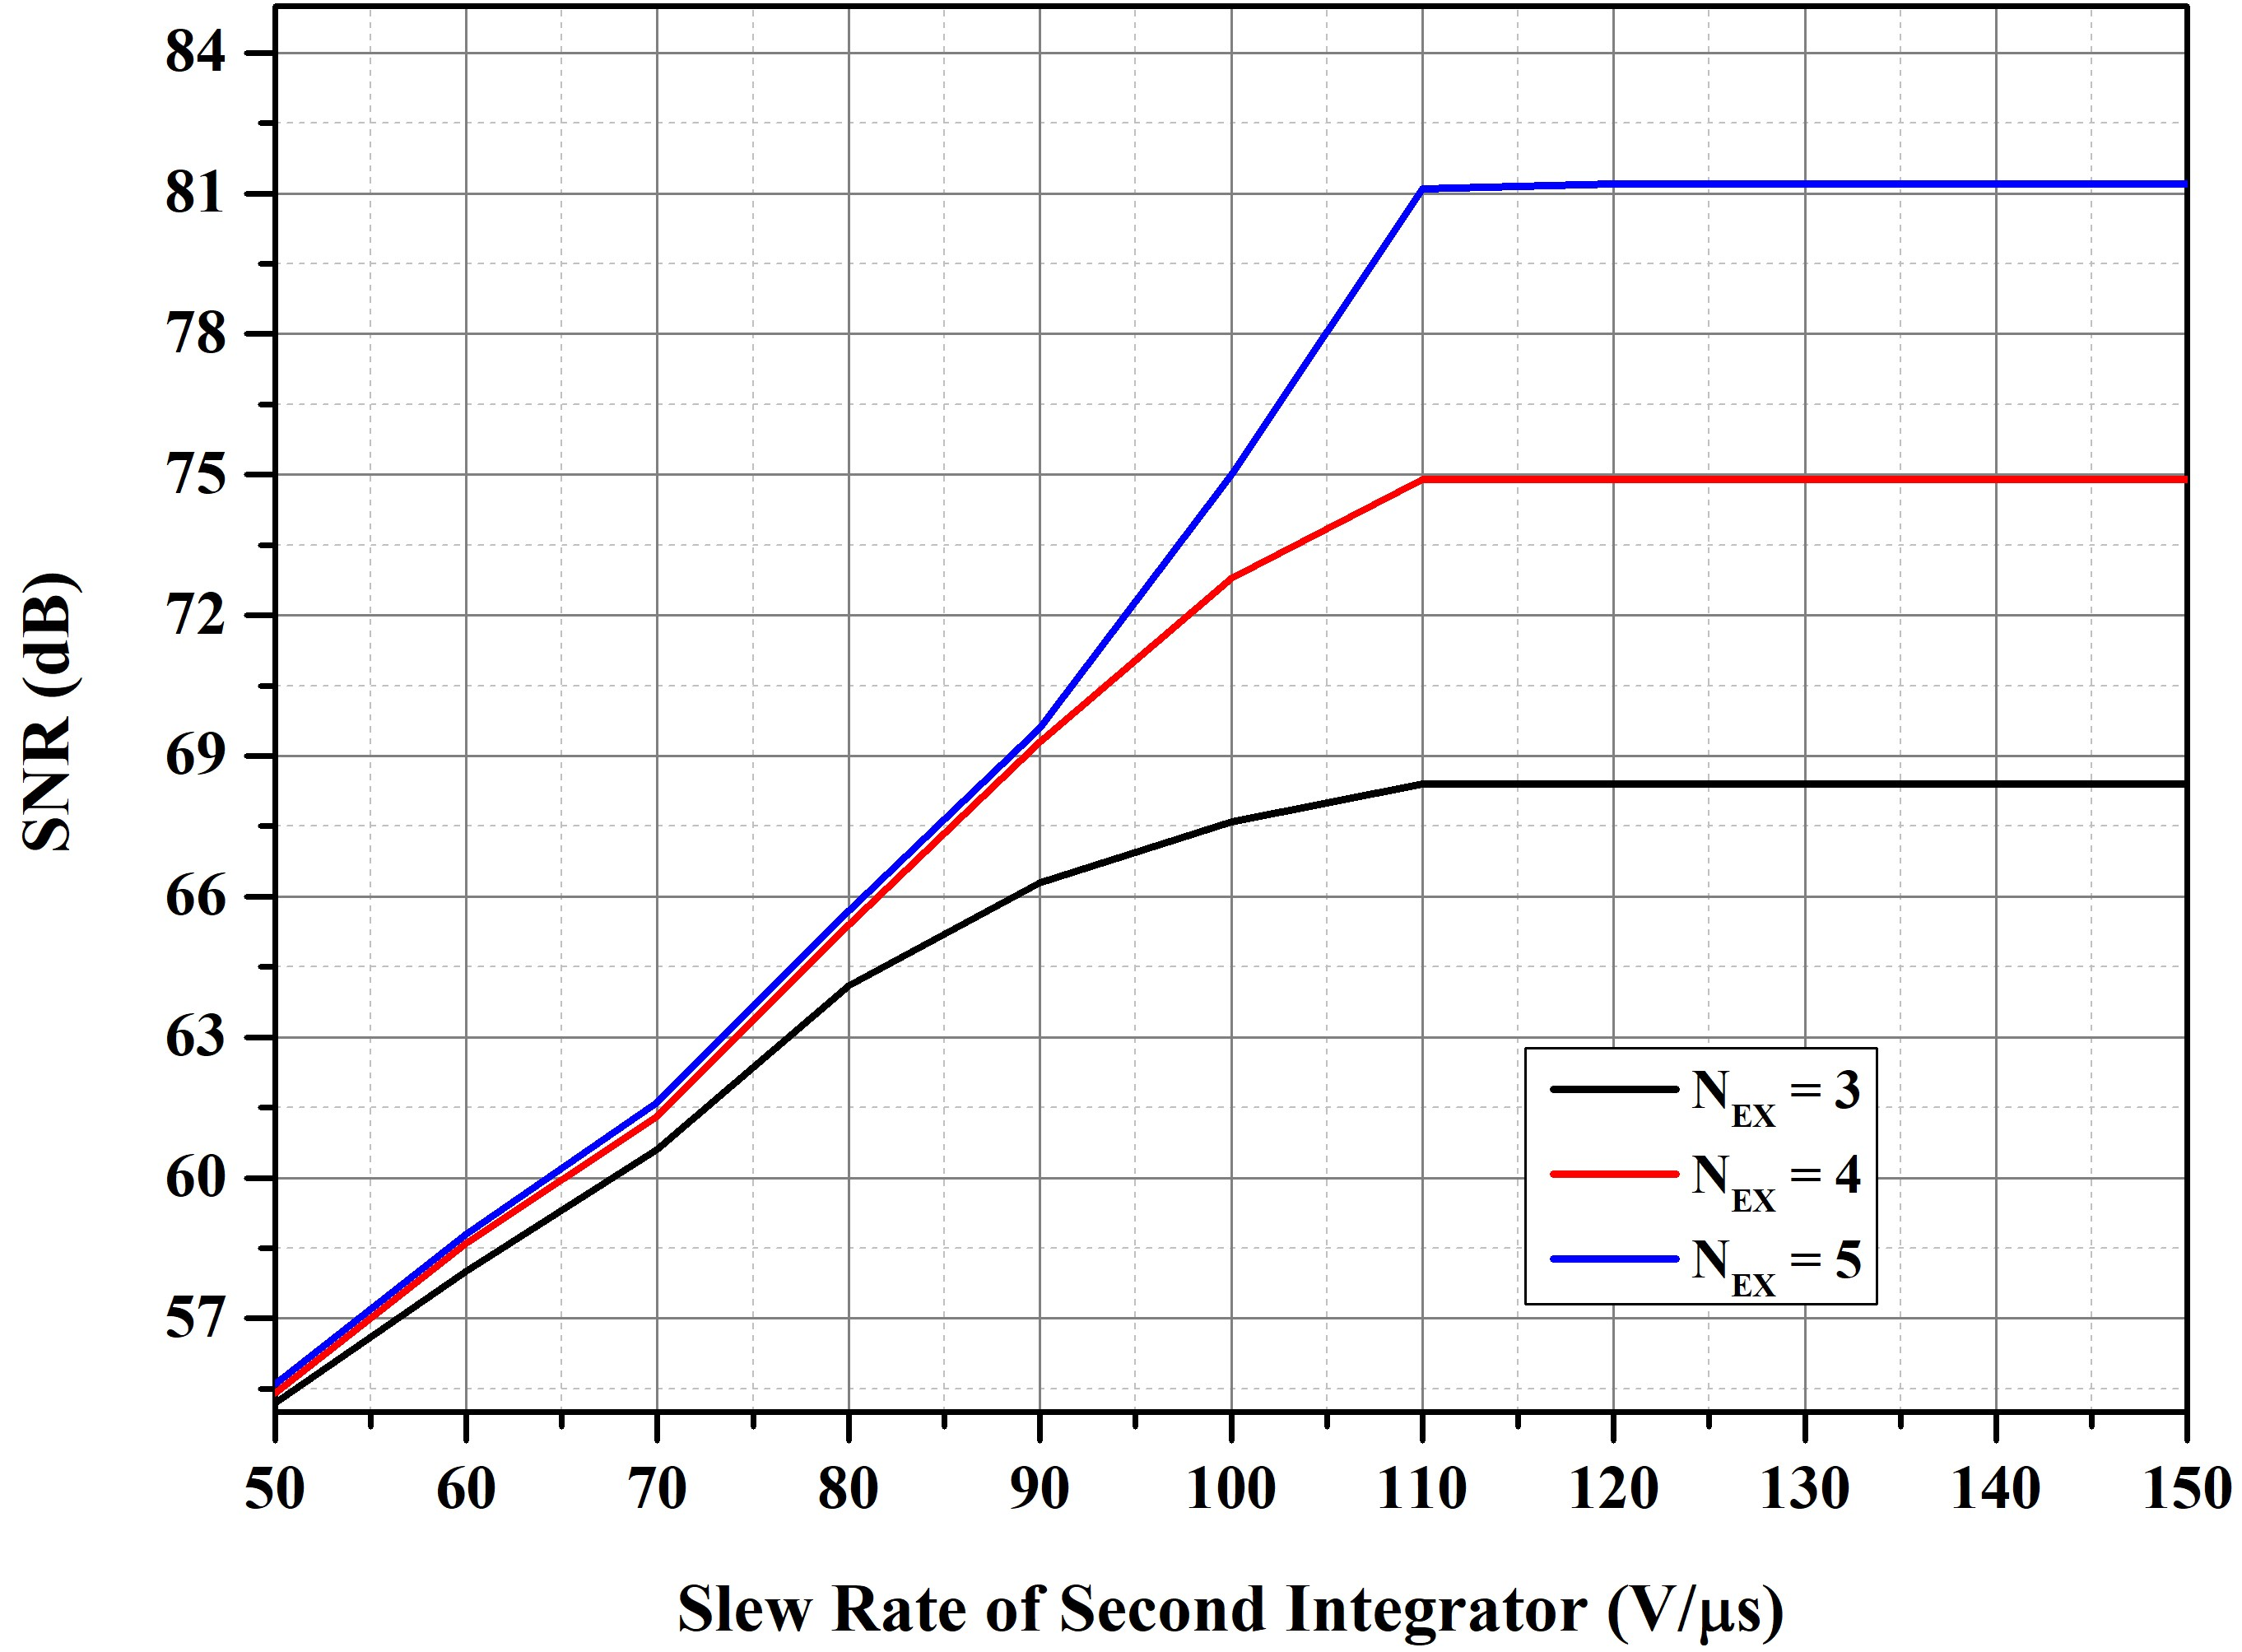
\includegraphics[scale=.28]{Chap04/Figures/snr_vs_sr2_nsd3.jpg}
%     }
%     \caption
%     {
%         (a) Slew Rate of the first Op-Amp Vs Overall SNR of the Extended Counting Incremental {\textSigma}{\textDelta} Modulator
%         (b) Slew Rate of the second Op-Amp Vs Overall SNR of the Extended Counting Incremental {\textSigma}{\textDelta} Modulator
%     }
%     \label{SR_Vs_SNR_NSD3}
% \end{figure}


% \begin{figure}[h]
%     \centering
%     \subfigure[]
%     {
%         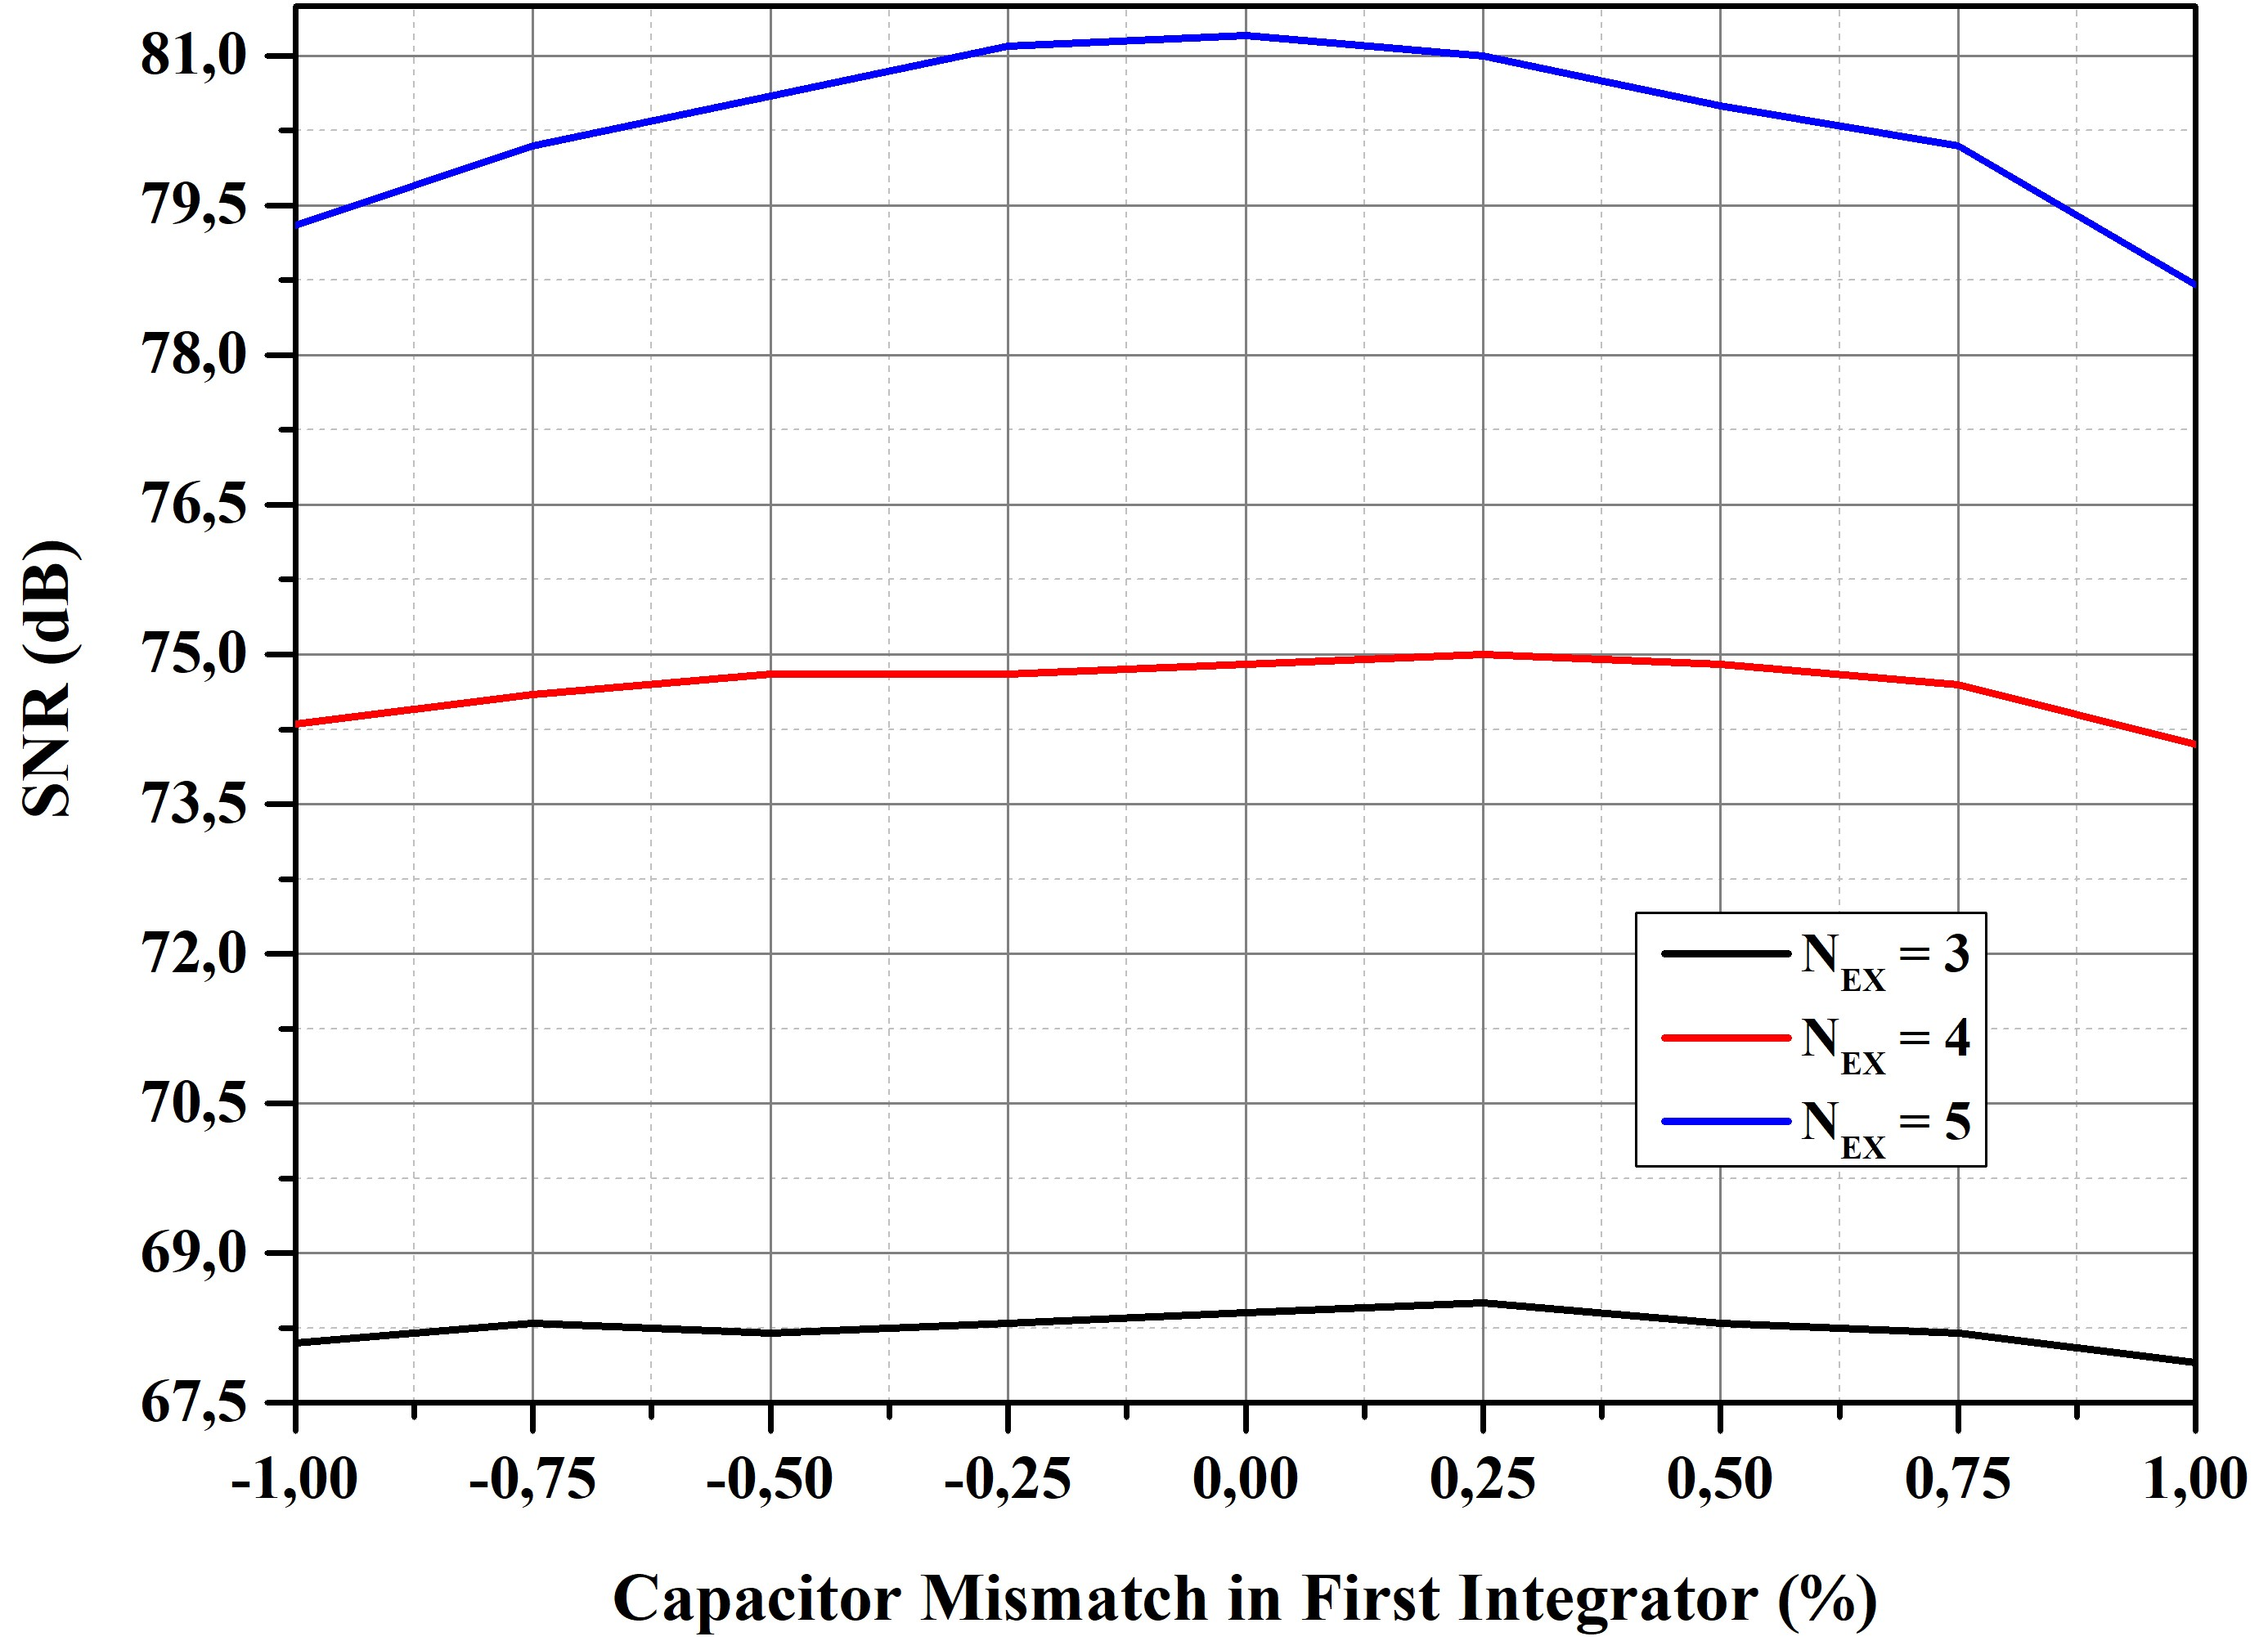
\includegraphics[scale=.28]{Chap04/Figures/snr_vs_capmis1_nsd3.jpg}
%     }
%     \qquad
%     \subfigure[]
%     {
%         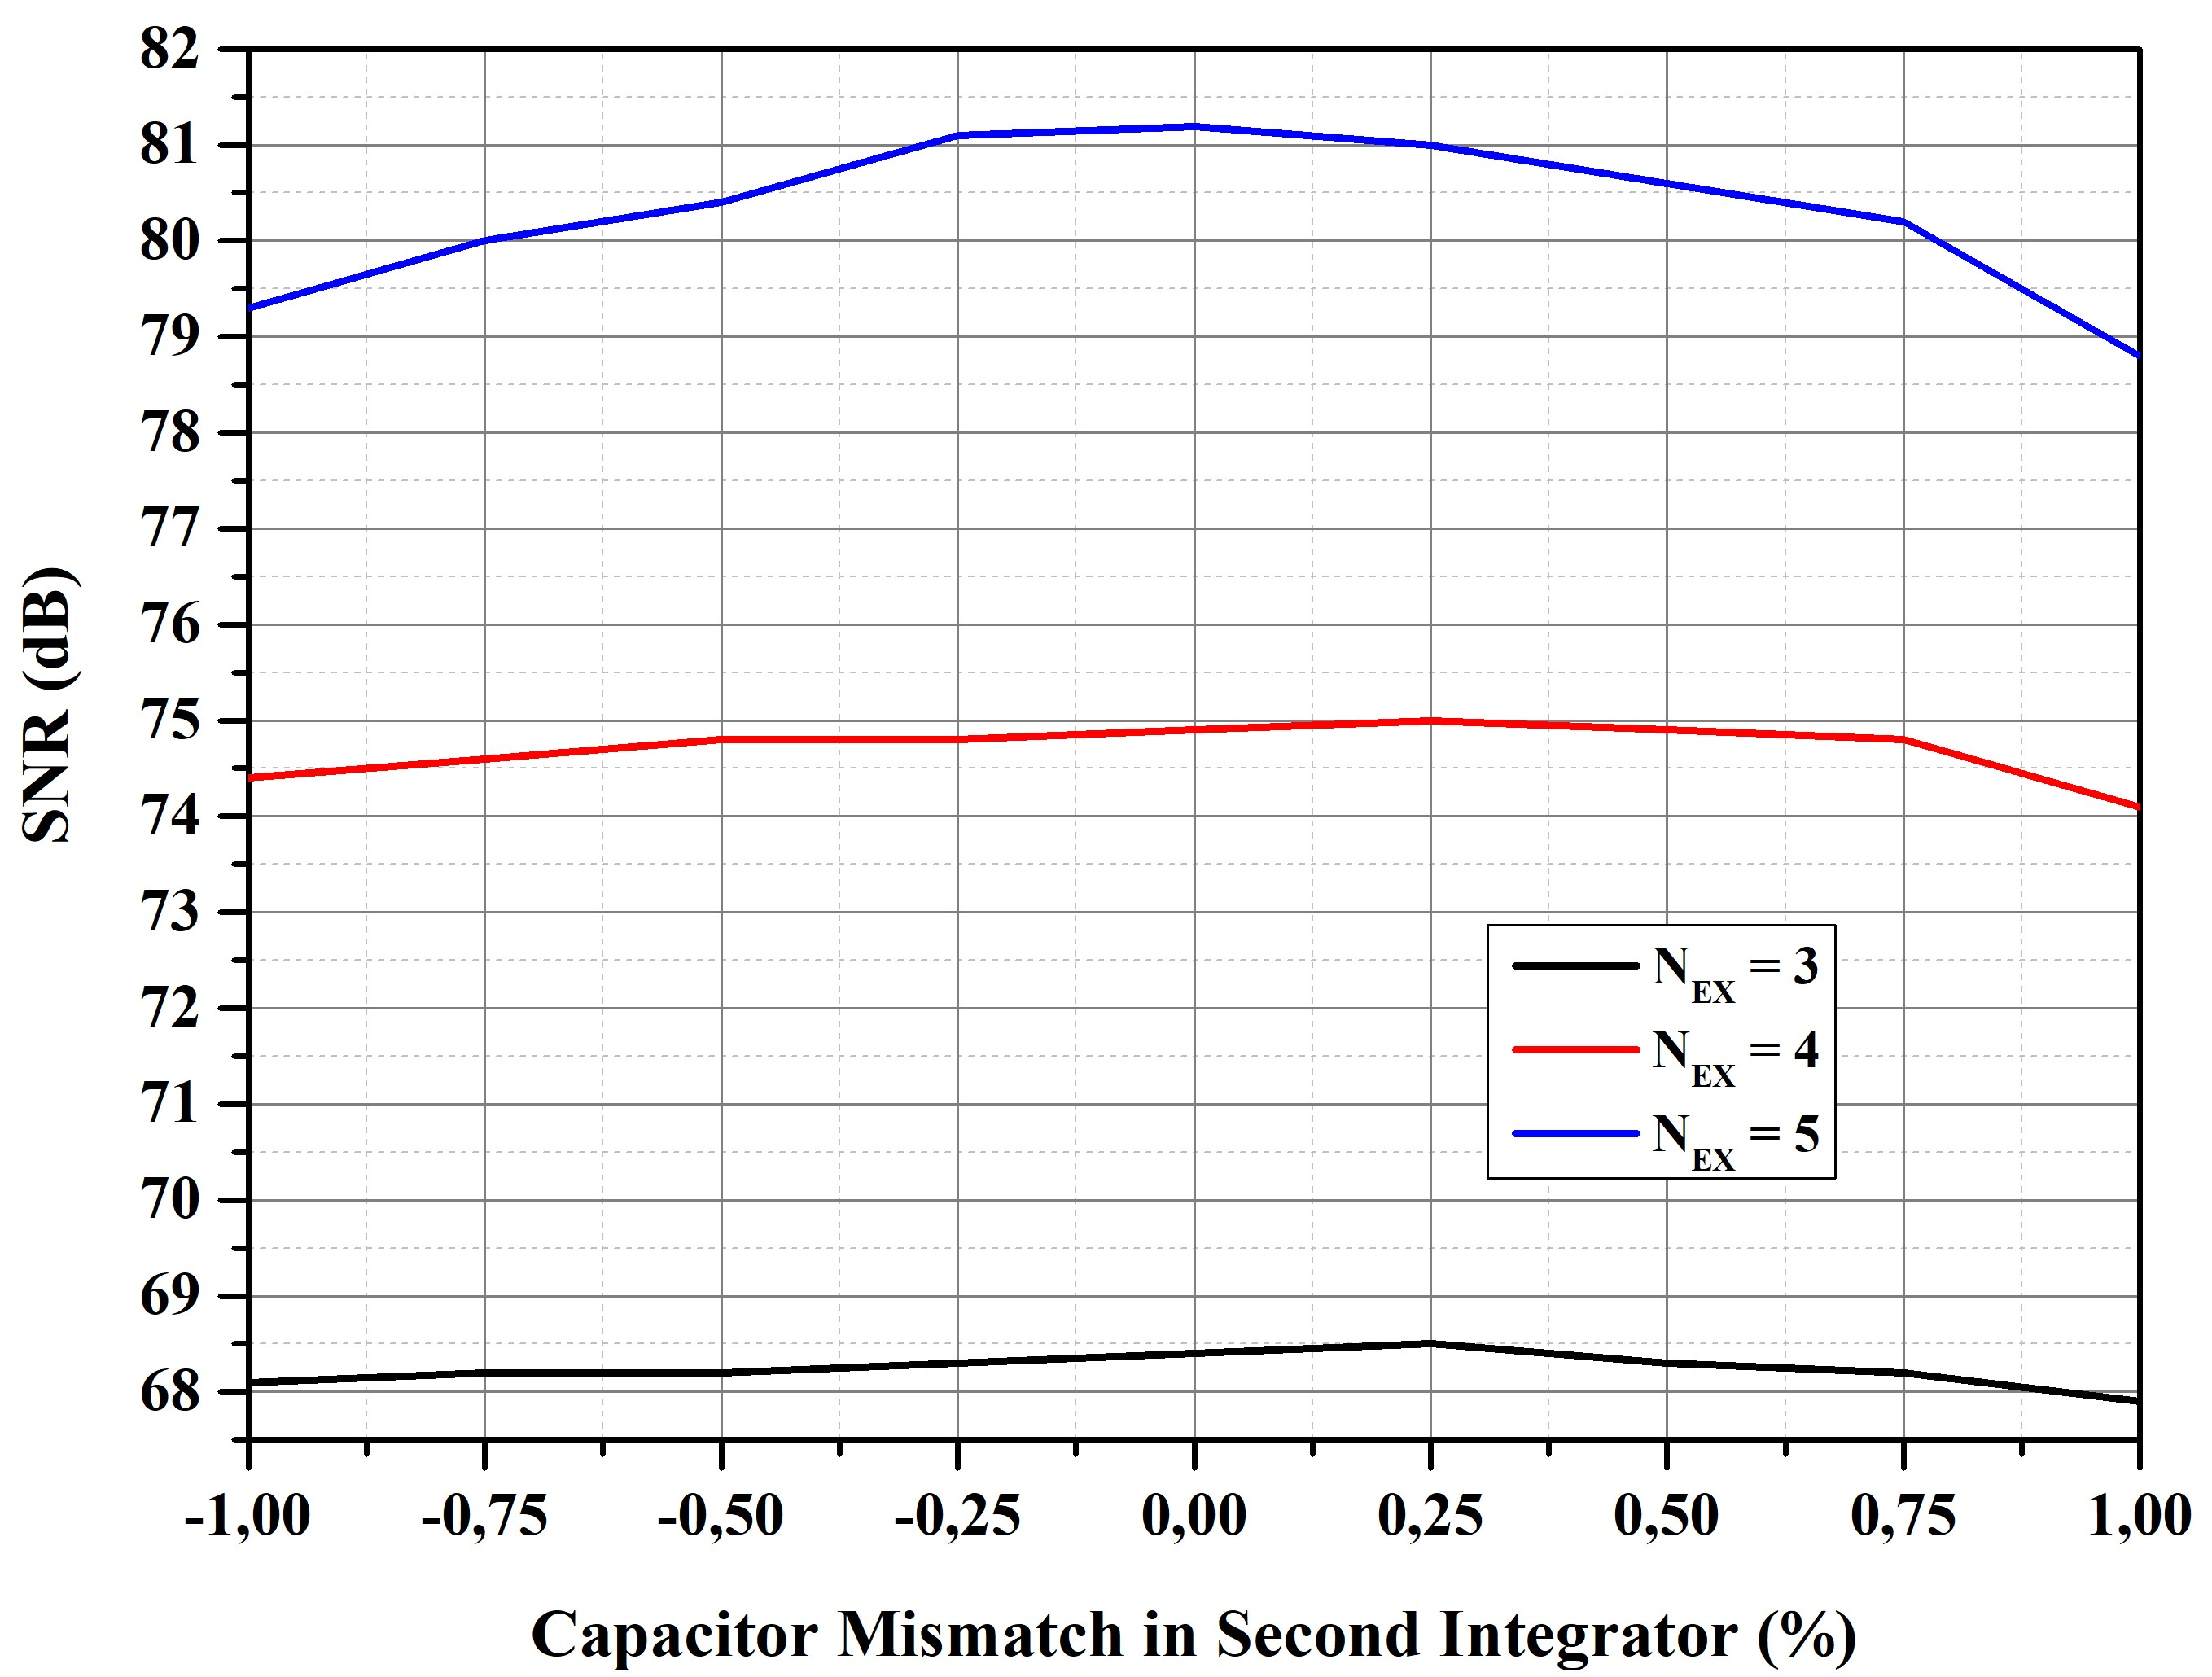
\includegraphics[scale=.28]{Chap04/Figures/snr_vs_capmis2_nsd3.jpg}
%     }
%     \caption
%     {
%         (a) Capacitor-mismatch of the first Op-Amp Vs Overall SNR of the Extended Counting Incremental {\textSigma}{\textDelta} Modulator
%         (b) Capacitor-mismatch of the second Op-Amp Vs Overall SNR of the Extended Counting Incremental {\textSigma}{\textDelta} Modulator
%     }
%     \label{CAPMIS_Vs_SNR_NSD3}
% \end{figure}
% A complete investigation done with all the non-idealities in the op-amps and the capacitor mismatch in the integartors are compiled and tabulated in the Table \ref{tab:OP_SPEC}. The comparison has to be made in order to decide the best possible solution for the given specifications of the ADC.
% % Please add the following required packages to your document preamble:
% % \usepackage[table,xcdraw]{xcolor}
% % If you use beamer only pass "xcolor=table" option, i.e. \documentclass[xcolor=table]{beamer}
% \begin{table}[h]
% \caption{Requirements of the Op-Amps for maximum SNDR}
% \label{tab:OP_SPEC}
% \resizebox{\textwidth}{!}{
% \begin{tabular}{c|c|c|c|c|c|c|c|c|c}
% \Xhline{4\arrayrulewidth}
% \textbf{Sr. No.} & \textbf{$N_{SD}$} & \textbf{$N_{EX}$} & \textbf{\begin{tabular}[c]{@{}c@{}}GBW of 1st\\ Op-Amp ($MHz$)\end{tabular}} & \textbf{\begin{tabular}[c]{@{}c@{}}SR of 1st\\ Op-Amp ($V/\mu s$)\end{tabular}} & \textbf{\begin{tabular}[c]{@{}c@{}}GBW of 2nd\\ Op-Amp ($MHz$)\end{tabular}} & \textbf{\begin{tabular}[c]{@{}c@{}}SR of 2nd\\ Op-Amp ($V/\mu s$)\end{tabular}} & \textbf{\begin{tabular}[c]{@{}c@{}}$\Delta$SNR (dB)\\ {[}1st Integ Cap mis{]}\end{tabular}} & \textbf{\begin{tabular}[c]{@{}c@{}}$\Delta$SNR (dB)\\ {[}2nd Integ Cap mis{]}\end{tabular}} & \textbf{\begin{tabular}[c]{@{}c@{}}SNR\\ (dB)\end{tabular}} \\ \Xhline{4\arrayrulewidth}
% \textbf{1} & 2 & 5 & 250 & 270 & 160 & 170 & -2.3 & -1.8 & 69.5 \\ 
% \textbf{2} &  & 6 & 250 & 270 & 160 & 170 & -5.9 & -5.1 & 76.2 \\ 
% \textbf{3} &  & 7 & 250 & 270 & 160 & 170 & -9.7 & -8.6 & 80.9 \\ \hline
% \textbf{4} & {\color[HTML]{CB0000} \textbf{3}} & 3 & 200 & 250 & 140 & 120 & -0.5 & -0.5 & 68.4 \\ 
% \textbf{5} &  & 4 & 200 & 250 & 140 & 120 & -0.8 & -0.8 & 74.9 \\ 
% \textbf{6} &  & {\color[HTML]{CB0000} \textbf{5}} & {\color[HTML]{CB0000} \textbf{200}} & {\color[HTML]{CB0000} \textbf{250}} & {\color[HTML]{CB0000} \textbf{140}} & {\color[HTML]{CB0000} \textbf{120}} & {\color[HTML]{CB0000} \textbf{-2.5}} & {\color[HTML]{CB0000} \textbf{-2.4}} & {\color[HTML]{CB0000} \textbf{81.2}} \\ \Xhline{4\arrayrulewidth}
% \end{tabular}
% }
% \end{table}
% The last column of Table \ref{tab:OP_SPEC} presents the overall SNDR for the giver combination of the resolution of the quantizers and the op-amp non-idealities taking into account (without capacitor mismatch). The cases which accomplish the demand of SNDR, even in the presence of non-idealities, are 3rd case with $N_{SD}=2$ \& $N_{EX}=7$ and 6th case where $N_{SD}=3$ \& $N_{EX}=5$. However, the architecture with $N_{SD}=3$ appears to have the relaxed requirements comparatively w.r.t. the one with $N_{SD}=2$ and it yields the required SNR even with the capacitor mismatch.

% In regards to the capacitor mismatch causing the coefficient variation of the integrator, the percentage of deterioration in the overall SNDR, comparing the two cases, is more in the architecture with $N_{SD}=2$. Therefore, from the comprehensive investigation conducted on the developed Simulink model of the Extended Range Incremental $\Sigma
% \Delta$ Modulator, the conclusion of selecting the combination of resolutions of $N_{SD}=3$ and $N_{EX}=5$ has been made and the block specifications are extracted with a sampling capacitor of size 400 $fF$. 